\documentclass[utf8]{beamer}
% \documentclass[utf8,aspectratio=169]{beamer}
\usecolortheme{seagull}
\usecolortheme{nicole}
\useinnertheme{nicole}
\useoutertheme{nicole}
\setbeamertemplate{navigation symbols}{}
\setbeamercovered{invisible}
\usepackage{color}

\usepackage[normalem]{ulem}
\DeclareRobustCommand{\hsout}[1]{\texorpdfstring{\sout{#1}}{#1}}

\AtBeginPart{\frame{\partpage}}

\author{~}
\title{Beyond\\ Consumer-Driven Contract Testing}
\subtitle{~}
\institute{~}
\date{~}

\usepackage[T1]{fontenc}
\usepackage{textcomp}
\usepackage[scaled=0.82]{beramono} % bitstream vera sans mono

\usepackage{tikz}
\usetikzlibrary{shapes,backgrounds,mindmap}

\usepackage{eso-pic}
\makeatletter
\AddToShipoutPicture{%
\begin{tikzpicture}%
% put: x (from left) , y (from bottom)
\put(240,10){
\includegraphics[width=4cm]{./logos/Nicole.png}}%
\end{tikzpicture}%
}
\makeatother

\definecolor[named]{keywords}{HTML}{005D35}
\definecolor[named]{comments}{HTML}{808080}
\definecolor[named]{identifiers}{HTML}{FF0000}
\colorlet{blockbackground}{black!5}
\setbeamercolor{blockbackground}{bg=blockbackground}
\definecolor[named]{strings}{HTML}{0000FF}

\usepackage[final]{listings}
\usepackage{textcomp} % for upquote in listings

% \include{progressbar}

\lstset{
	keywordstyle=,%\bfseries,%RoyalBlue
	basicstyle=\footnotesize\ttfamily,
	%identifierstyle=\color{identifiers},
	commentstyle=\color{comments}\ttfamily\itshape,%Green
	stringstyle=\color{strings},
	%numbers=left,
	%numberstyle=\scriptsize,%\tiny
	%stepnumber=1,
	%numbersep=8pt,
	showstringspaces=false,
	breaklines=true,
	frameround=ffff,
	frame=single,
	tabsize=4,
	backgroundcolor=\color{blockbackground},
	rulecolor=\color{blockbackground},
	inputencoding=latin1,
	emphstyle=\color{red},
	texcl=true,
	numbersep=0pt,
	upquote=true
}

\lstnewenvironment{highlight}[1]{\lstset{basicstyle=\footnotesize\ttfamily\alt<#1>{}{\color{\greyedout}}}}{}

\begin{document}
{
	\usebackgroundtemplate{} % required, otherwise the tikzpicture does not get displayed
	\begin{frame}[t,plain]
		\titlepage
	\end{frame}
}
%%%%%%%%%%%%%%%%%%%%%%%%%%%%%%%%%%%%%%%%%%%%%%%%%%
\begin{frame}[fragile]{Soooo...}

\begin{itemize}

\item We want to build this nice webapp / distributed system / these microservices

\item We want to make sure ``Frontend'' and ``Backend'' play nicely together

\onslide<2->
\vspace{1.5em}
\item HOW???

\end{itemize}

\end{frame}

%%%%%%%%%%%%%%%%%%%%%%%%%%%%%%%%%%%%%%%%%%%%%%%%%%
\begin{frame}[fragile]{}

\begin{center}
{\Huge
``Super-Na\"ive'' Approach
}
\end{center}

\end{frame}

\begin{frame}[fragile]{}

\only<1>{
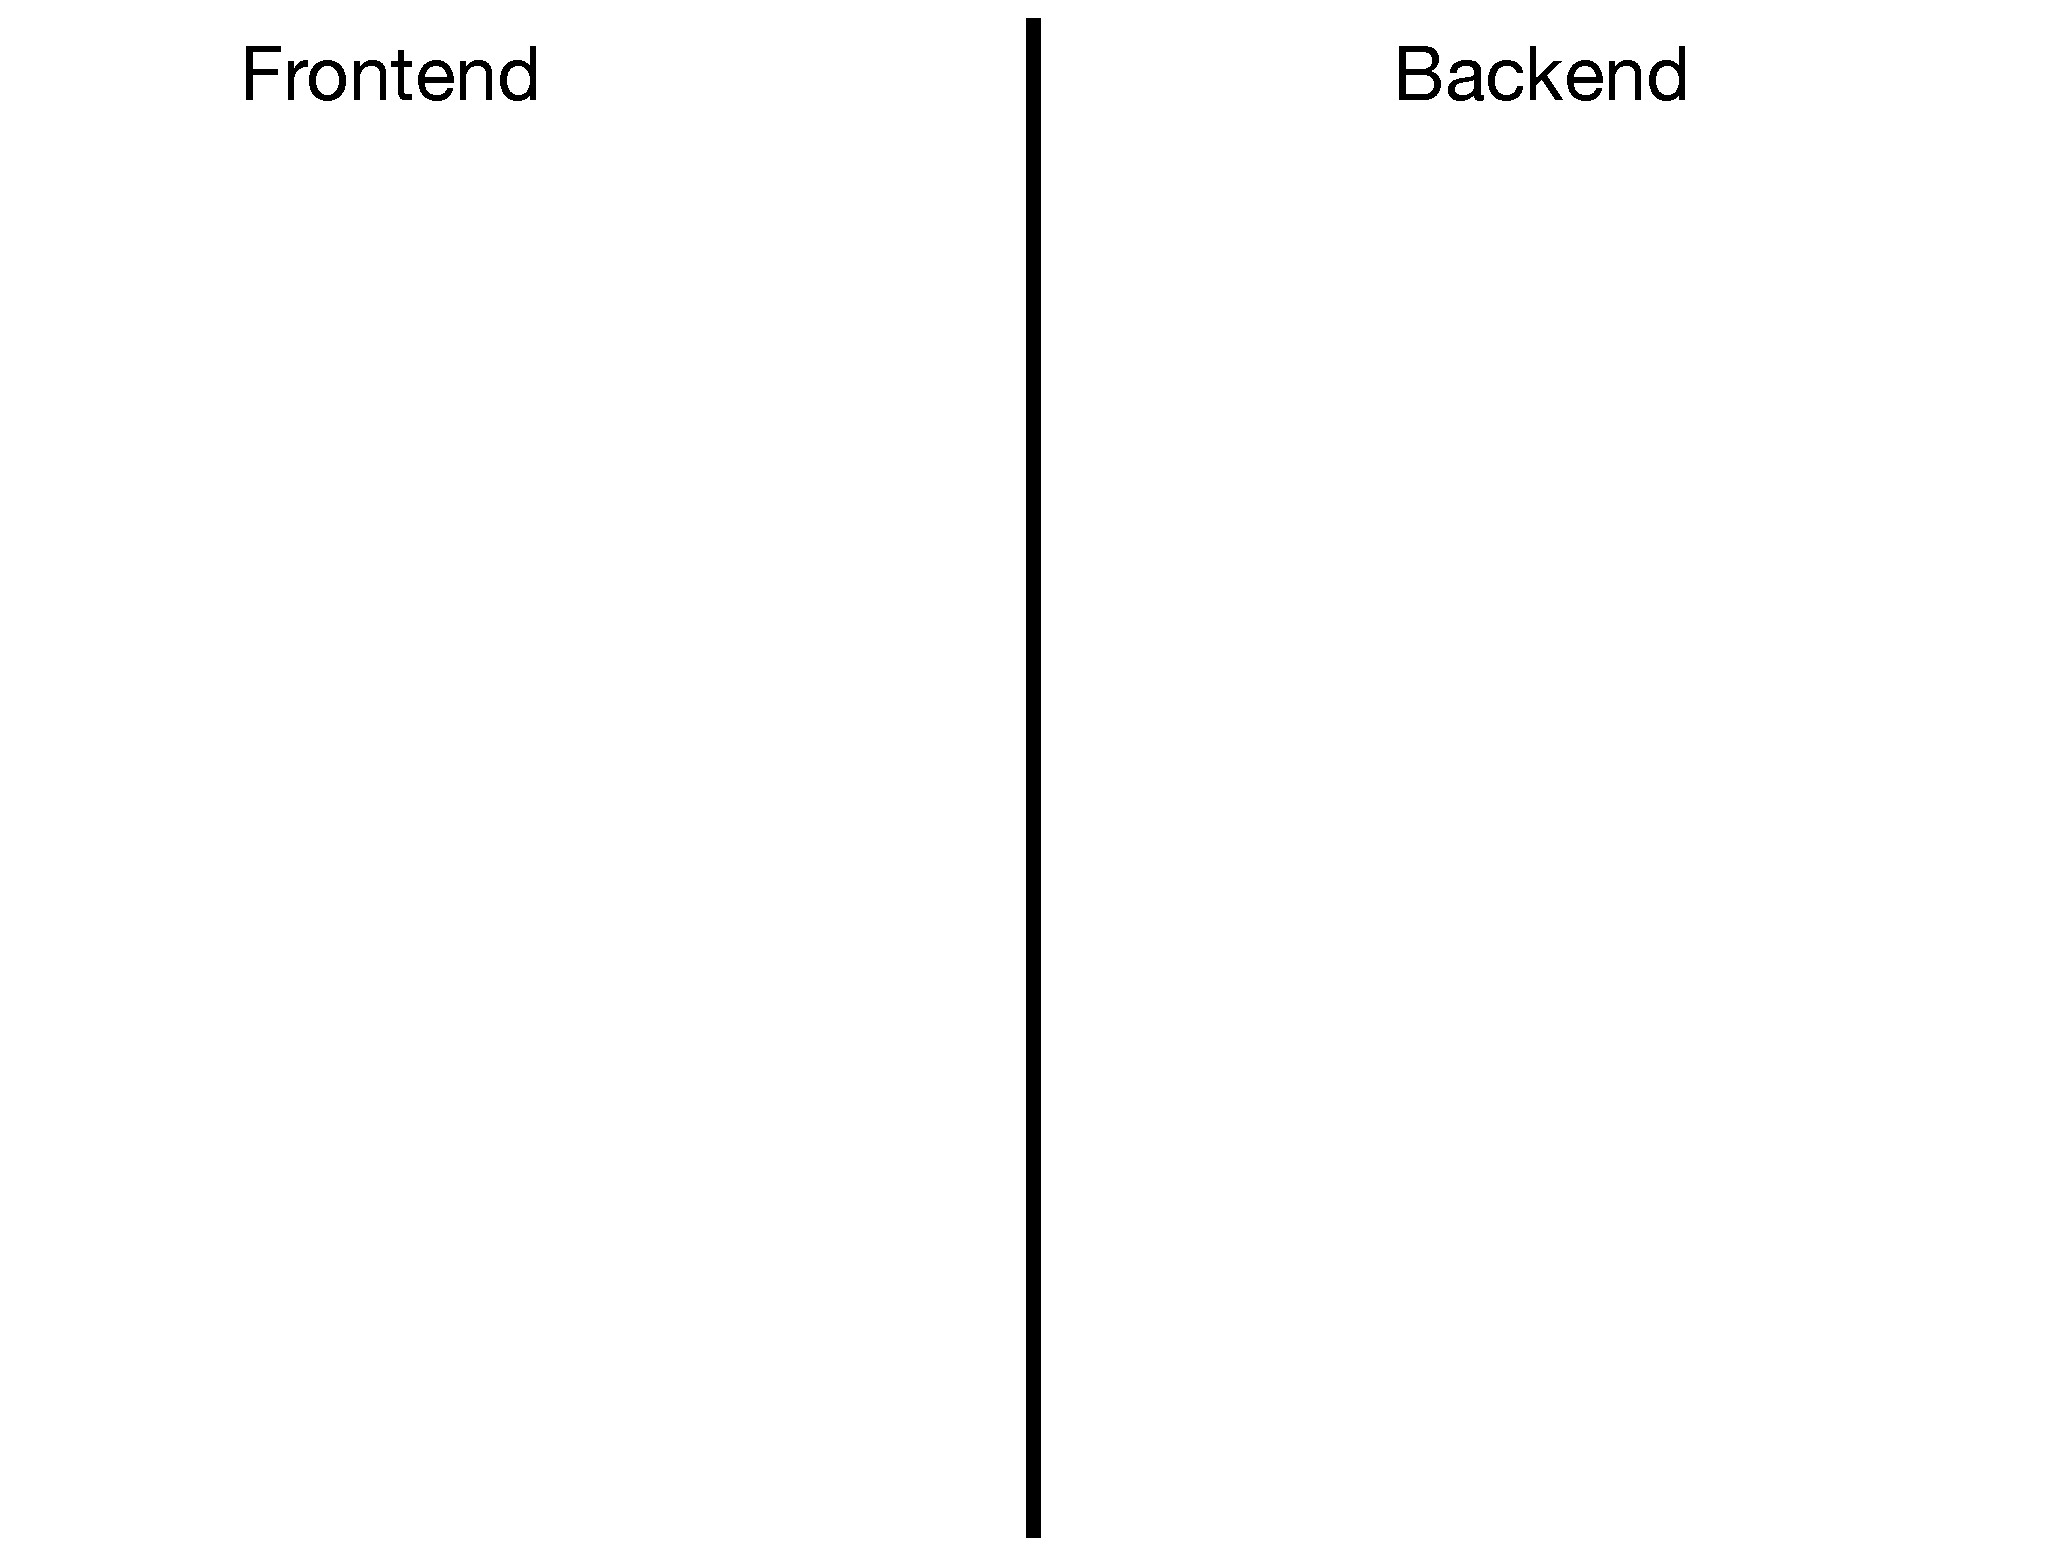
\includegraphics[width=\textwidth]{images/super-naive-approach-0.pdf}
}

\only<2>{
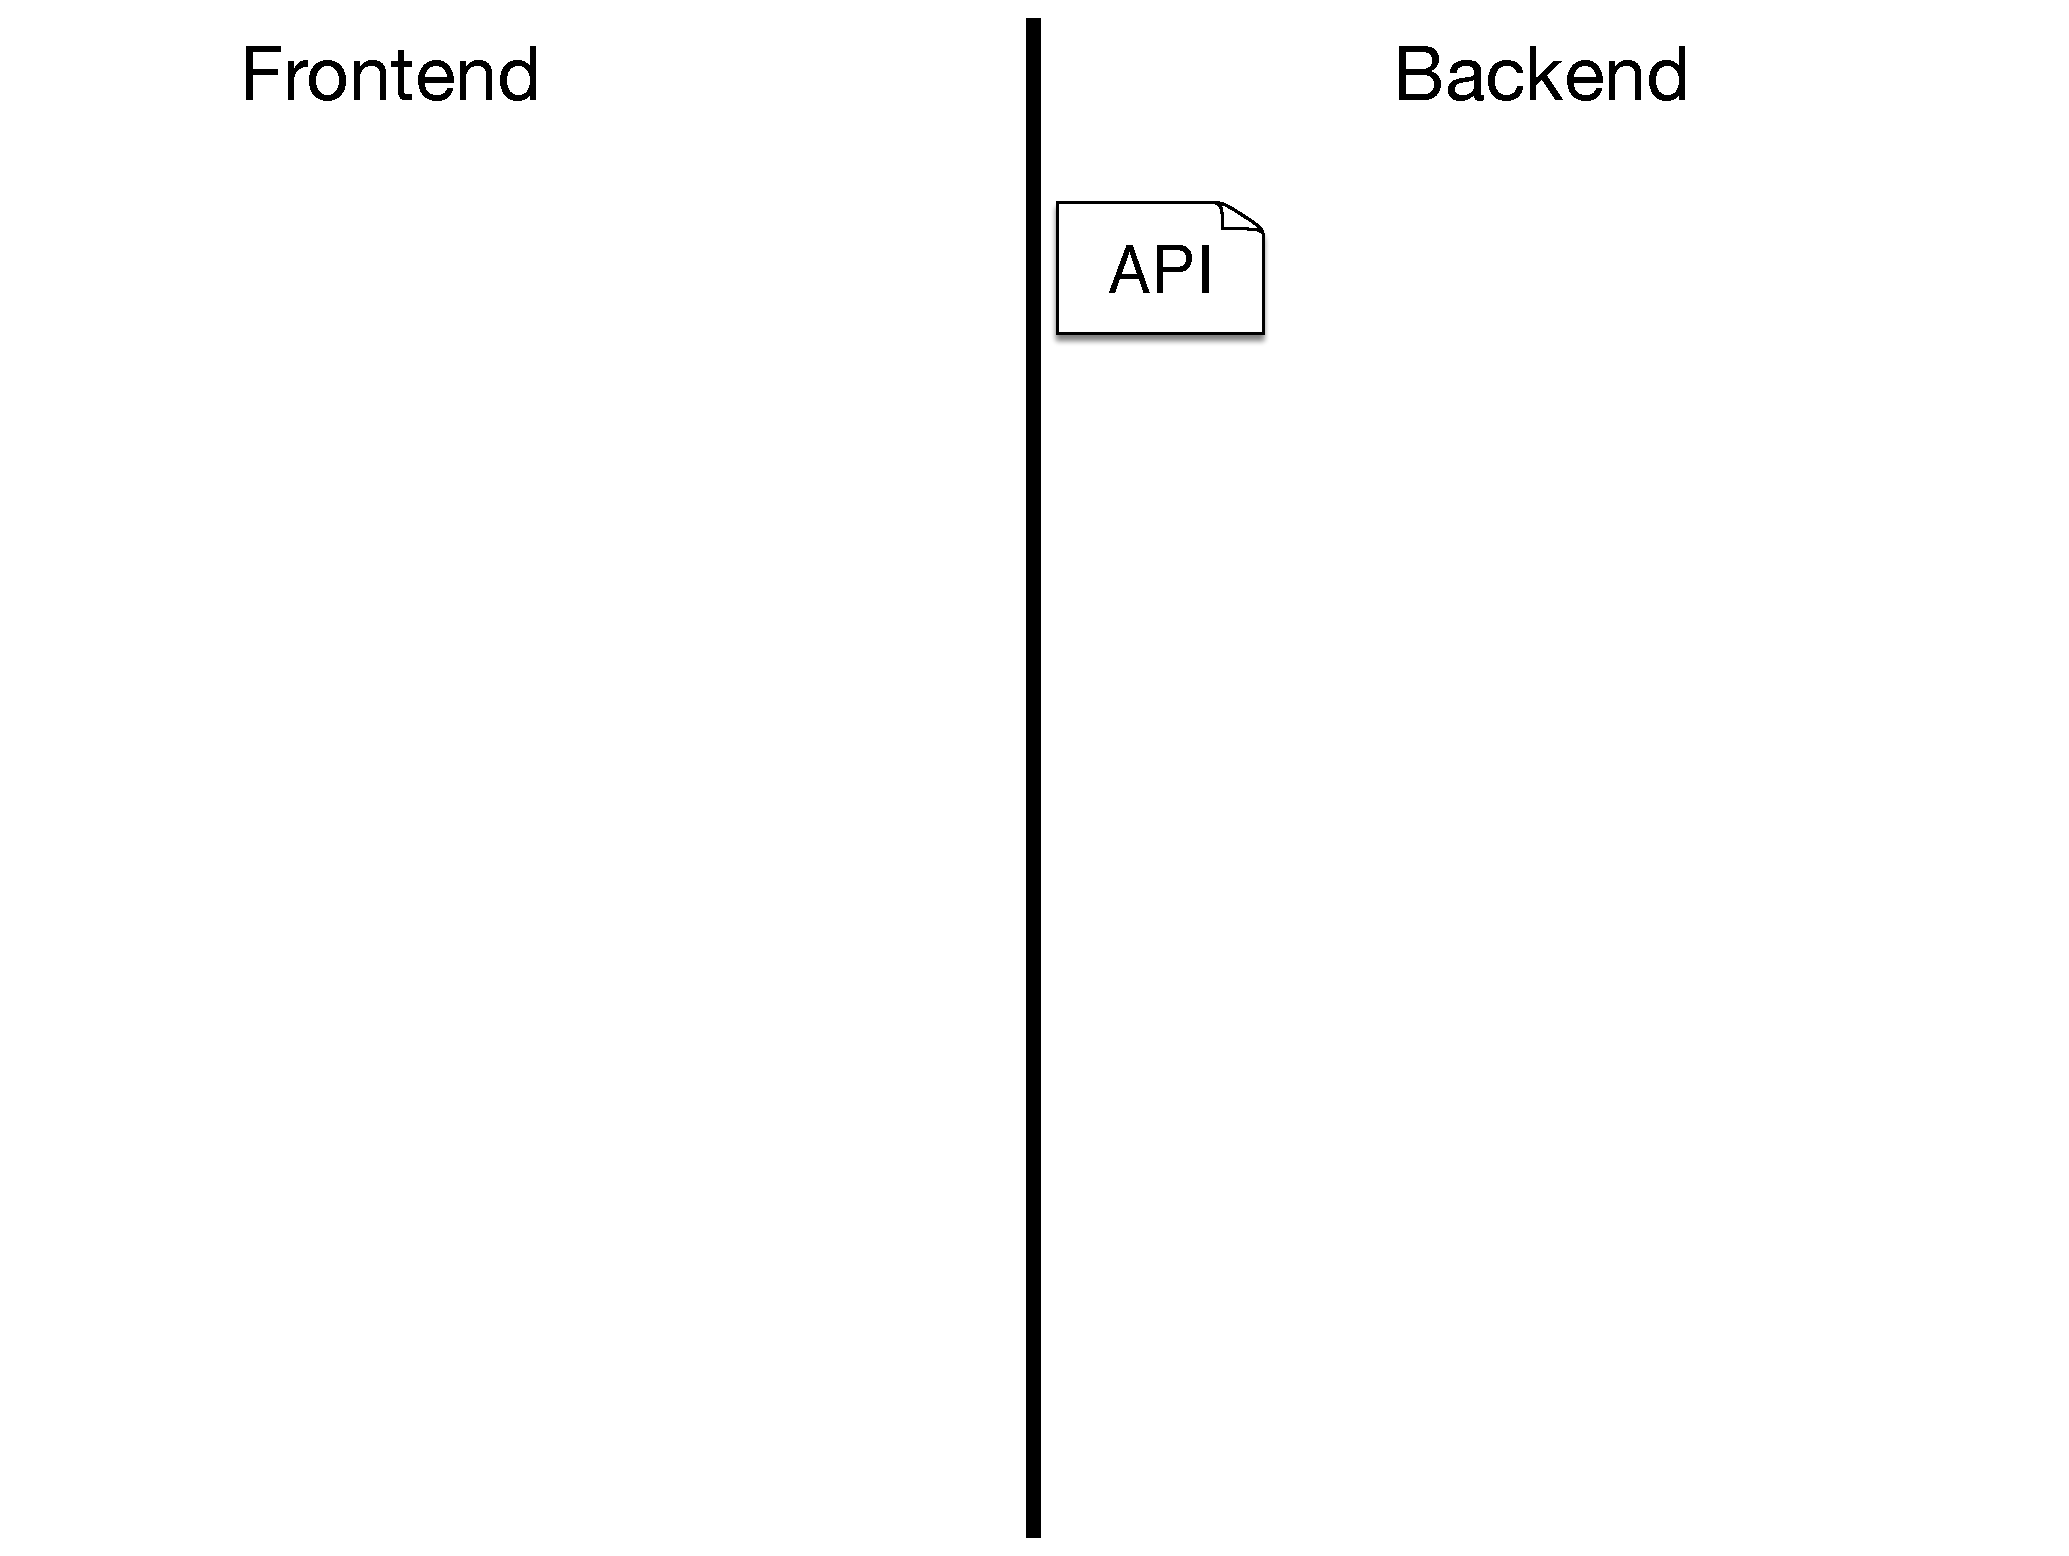
\includegraphics[width=\textwidth]{images/super-naive-approach-1.pdf}
}

\only<3>{
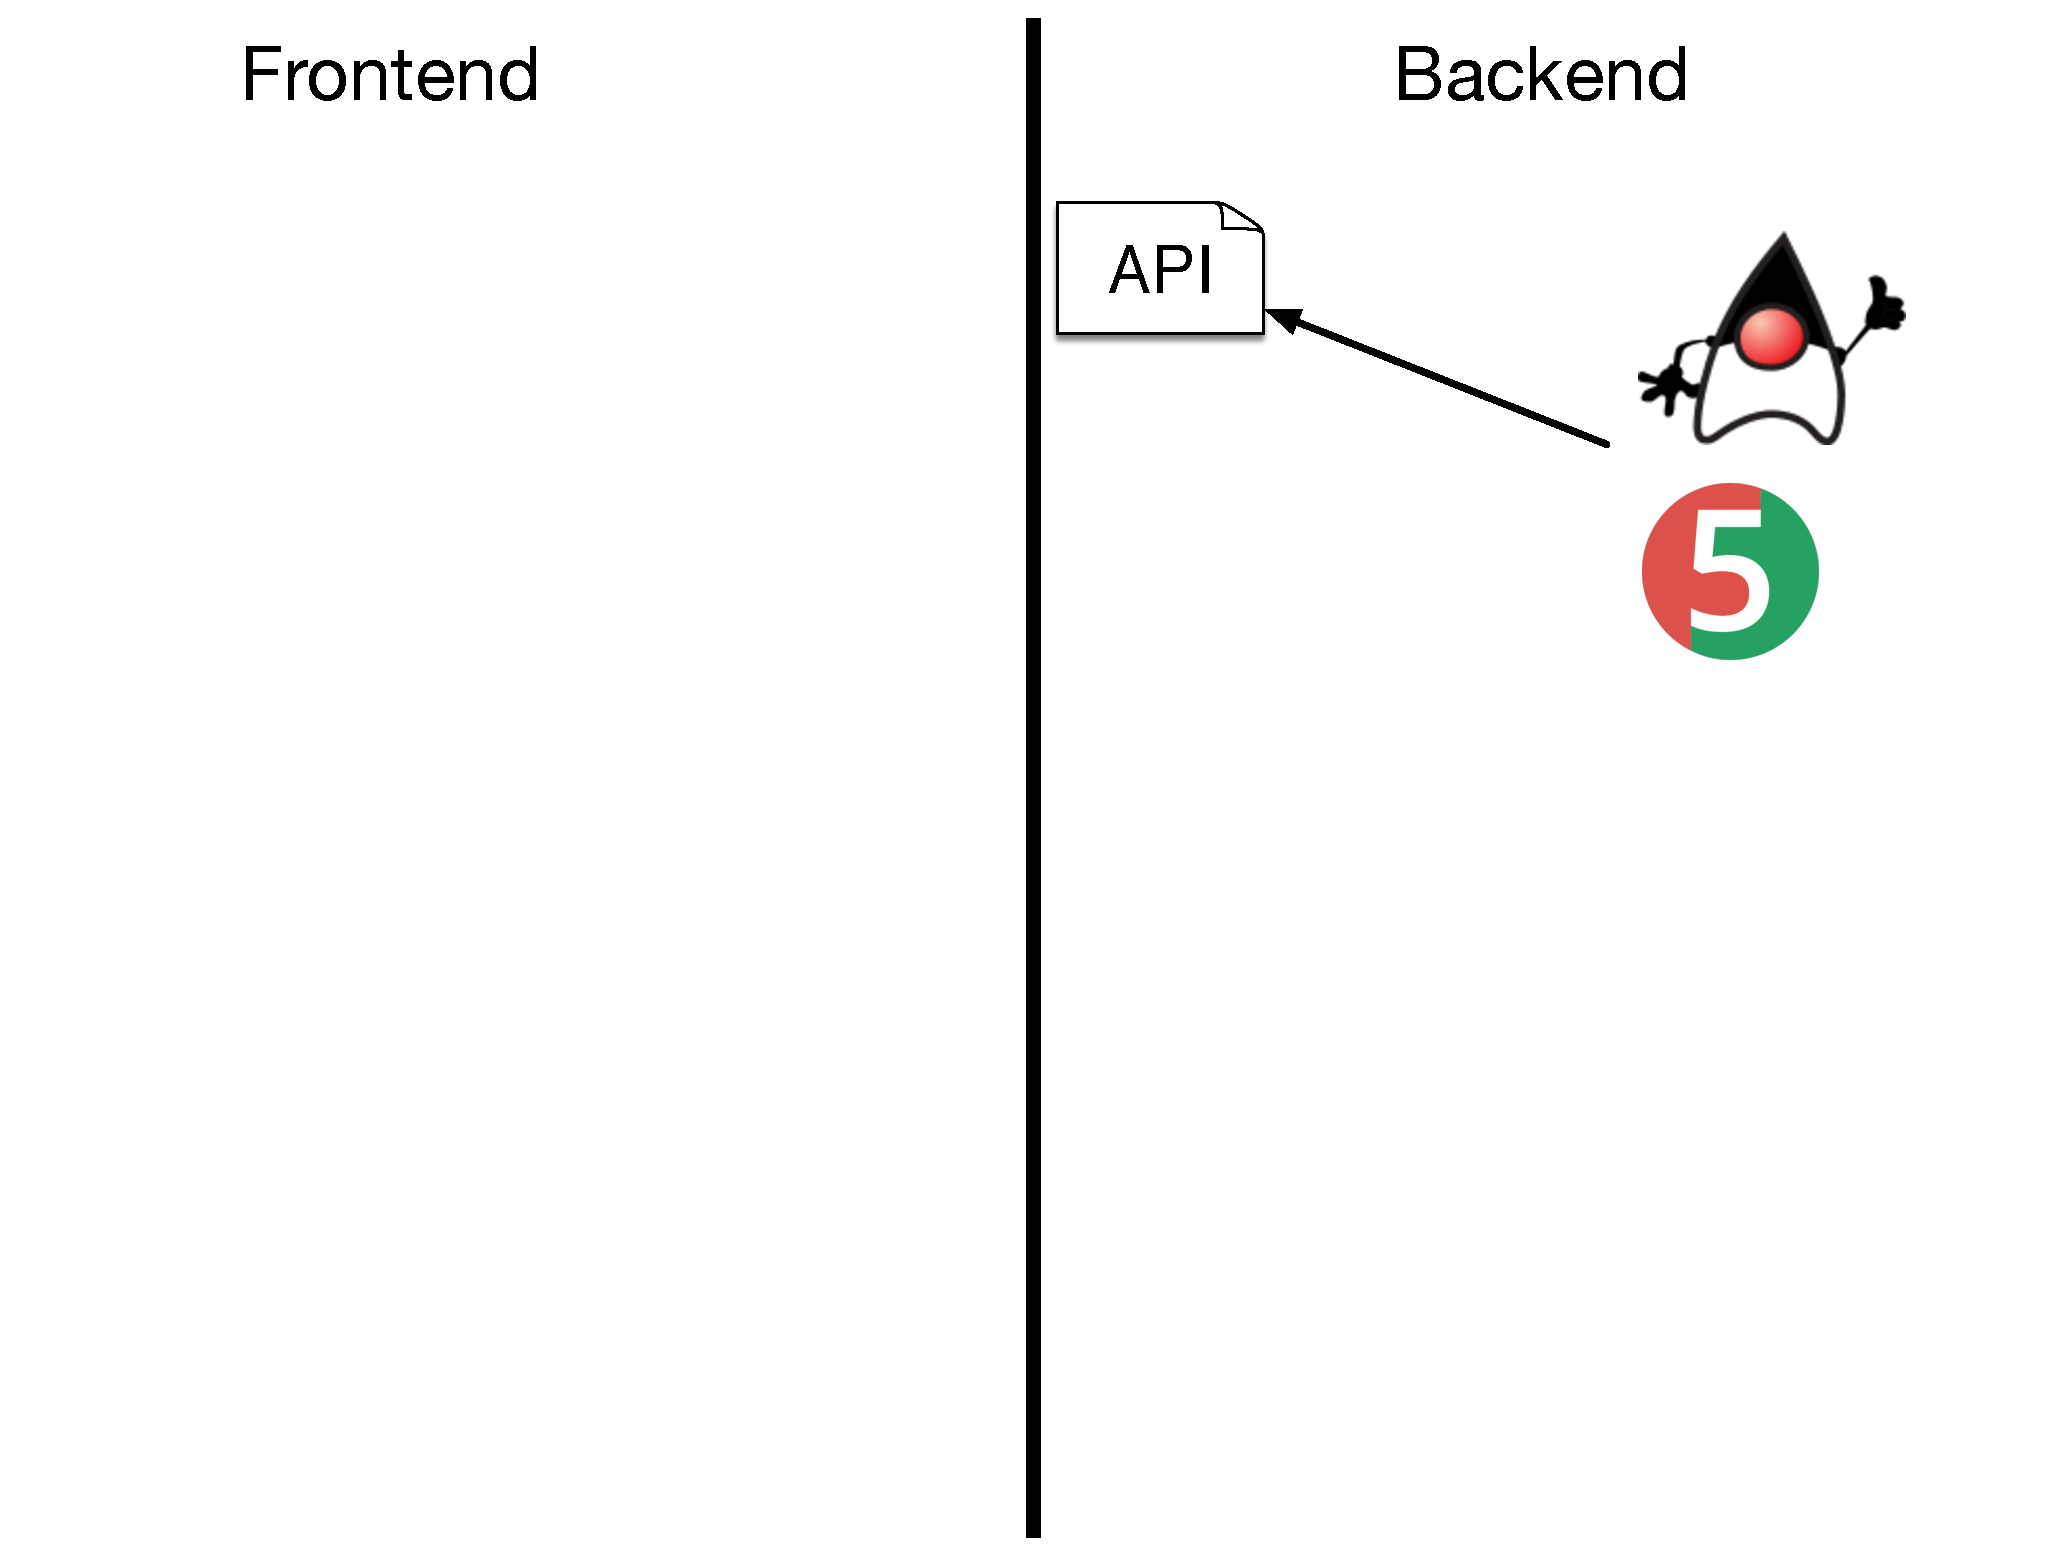
\includegraphics[width=\textwidth]{images/super-naive-approach-2.pdf}
}

\only<4>{
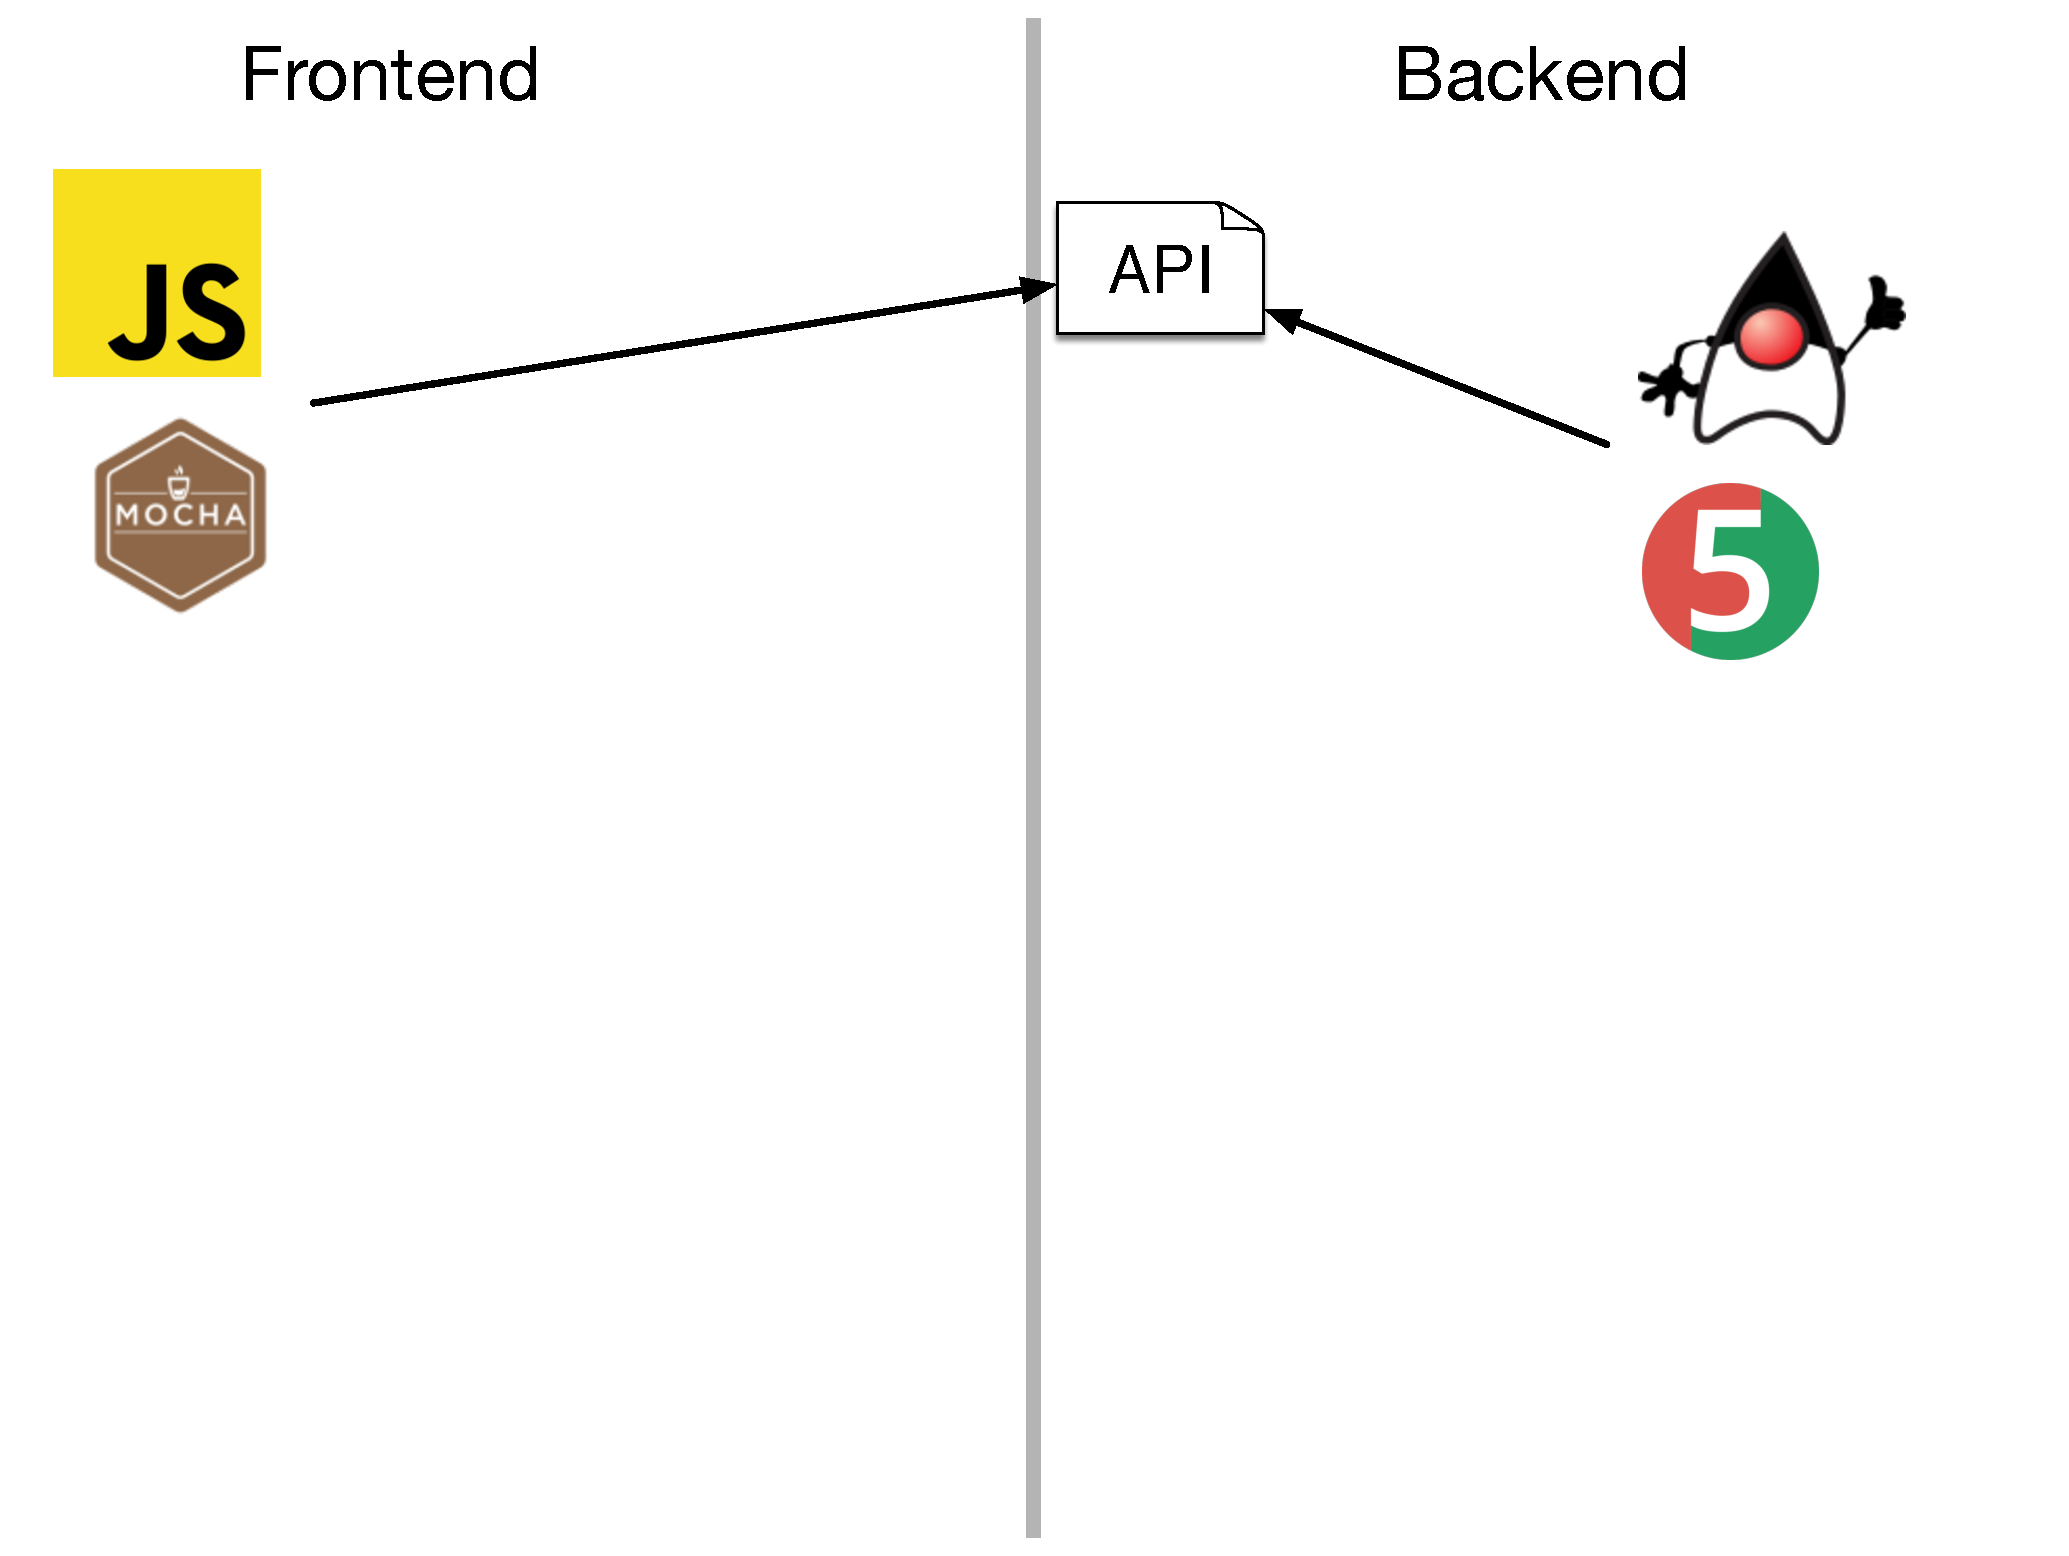
\includegraphics[width=\textwidth]{images/super-naive-approach-3.pdf}
}

\only<5>{
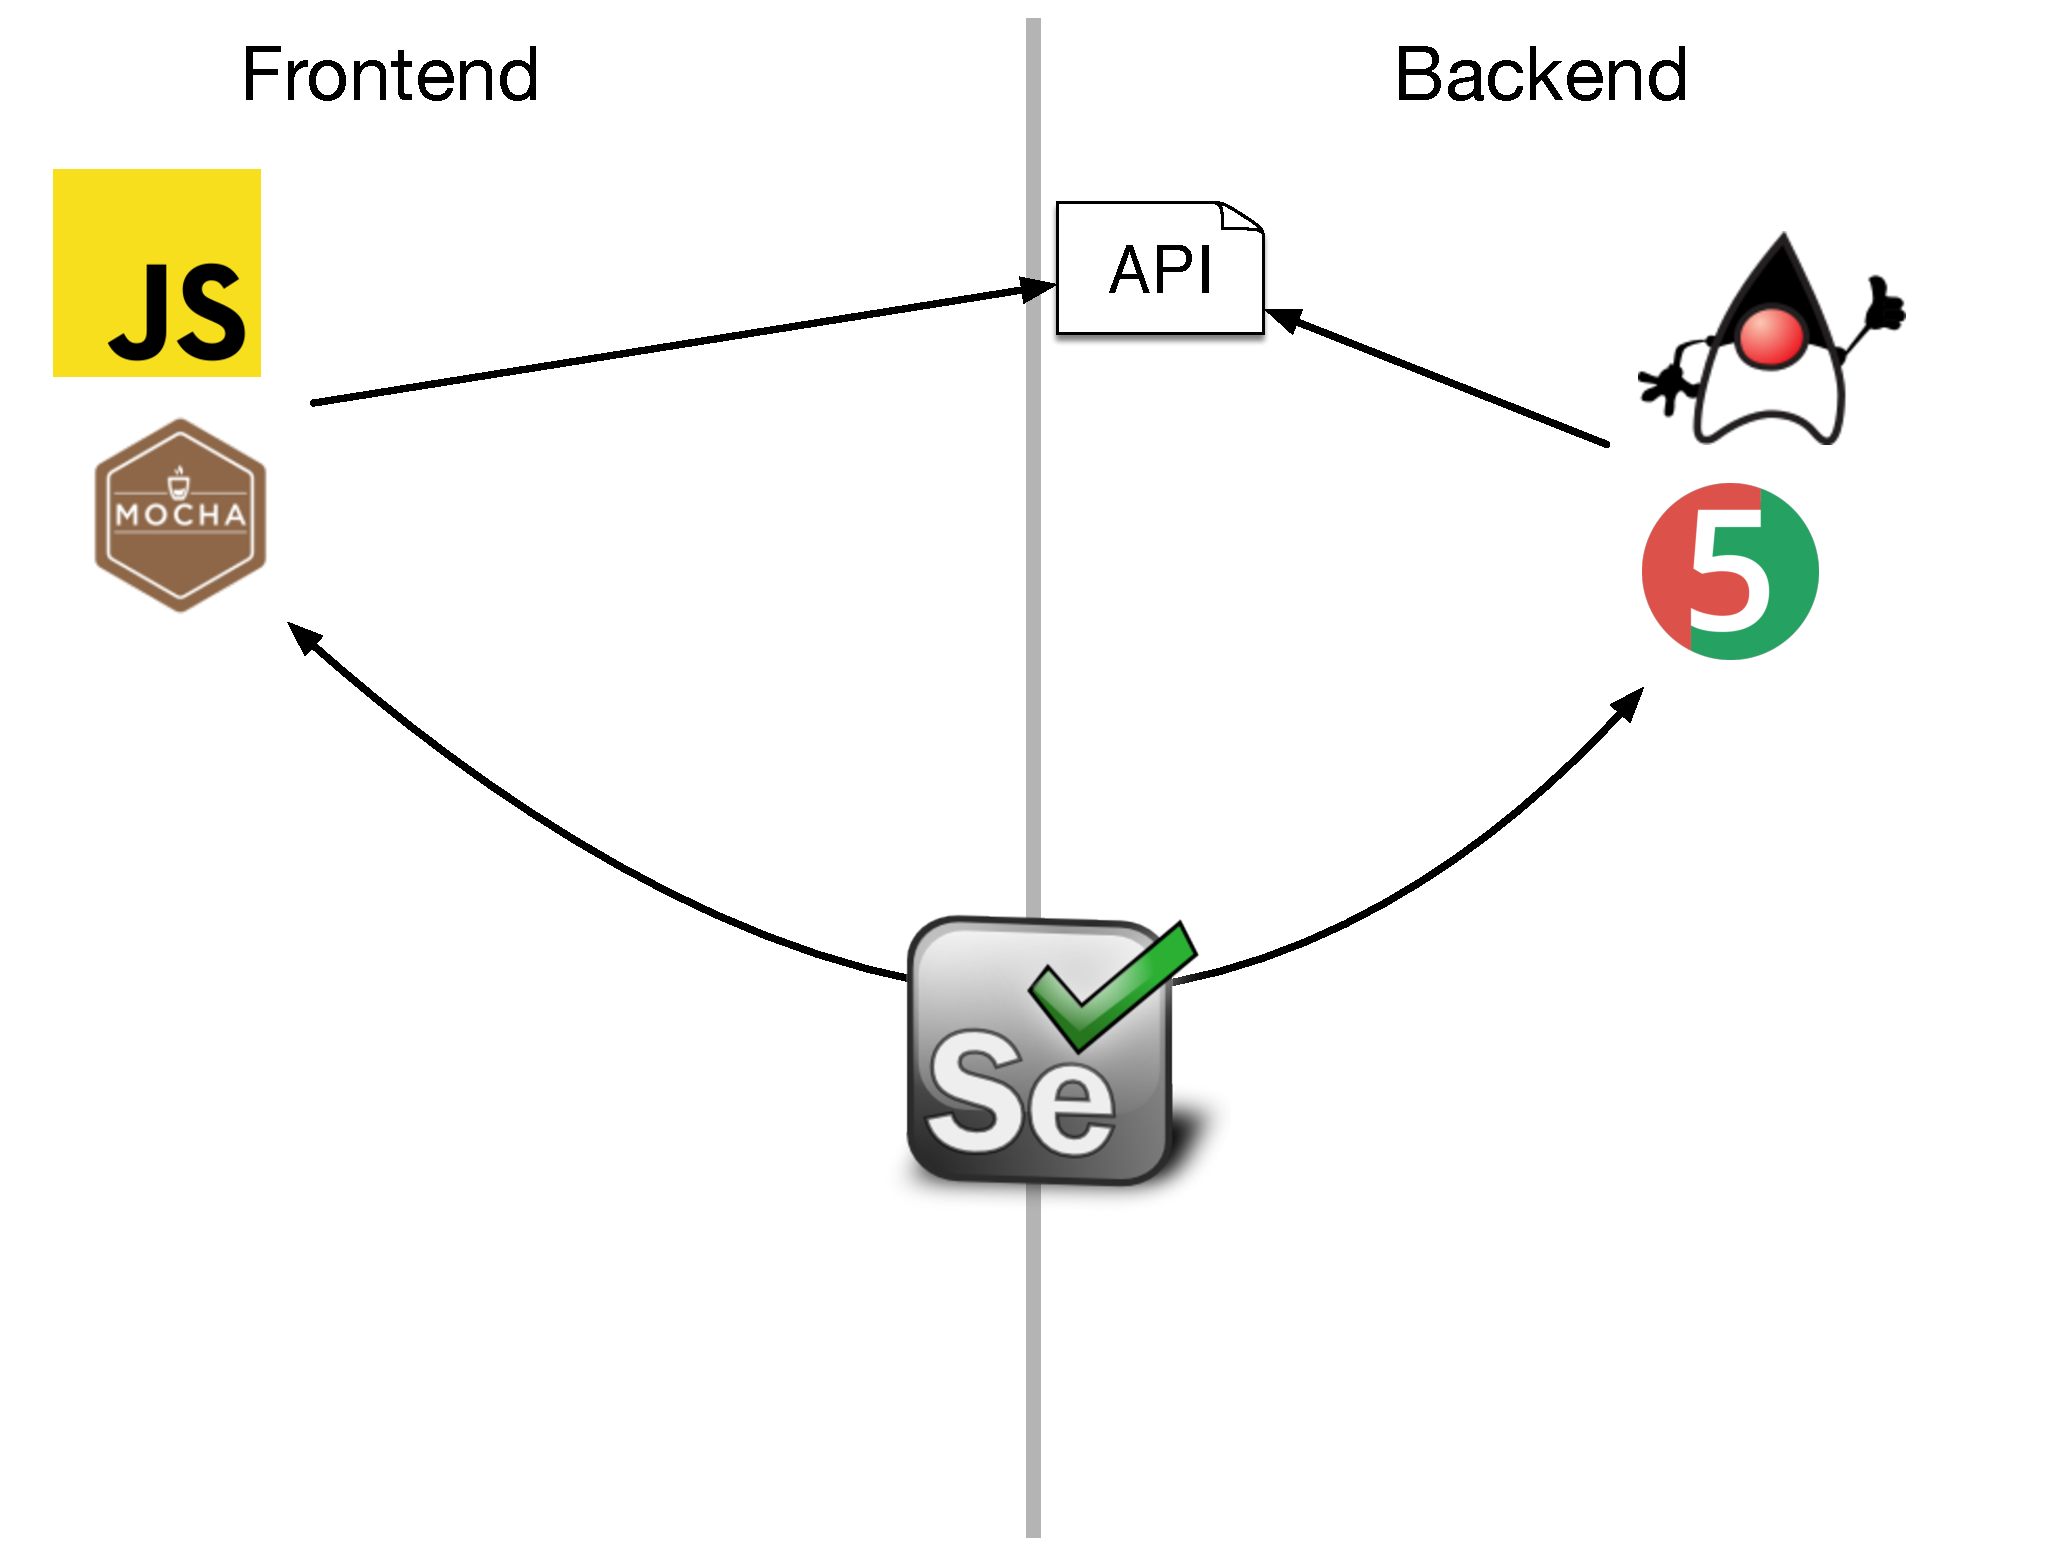
\includegraphics[width=\textwidth]{images/super-naive-approach-4.pdf}
}

\end{frame}

\begin{frame}[fragile]{}

\begin{center}
{\Huge
But $\ldots$
}
\end{center}

\end{frame}

\begin{frame}[fragile]{}

\only<1>{
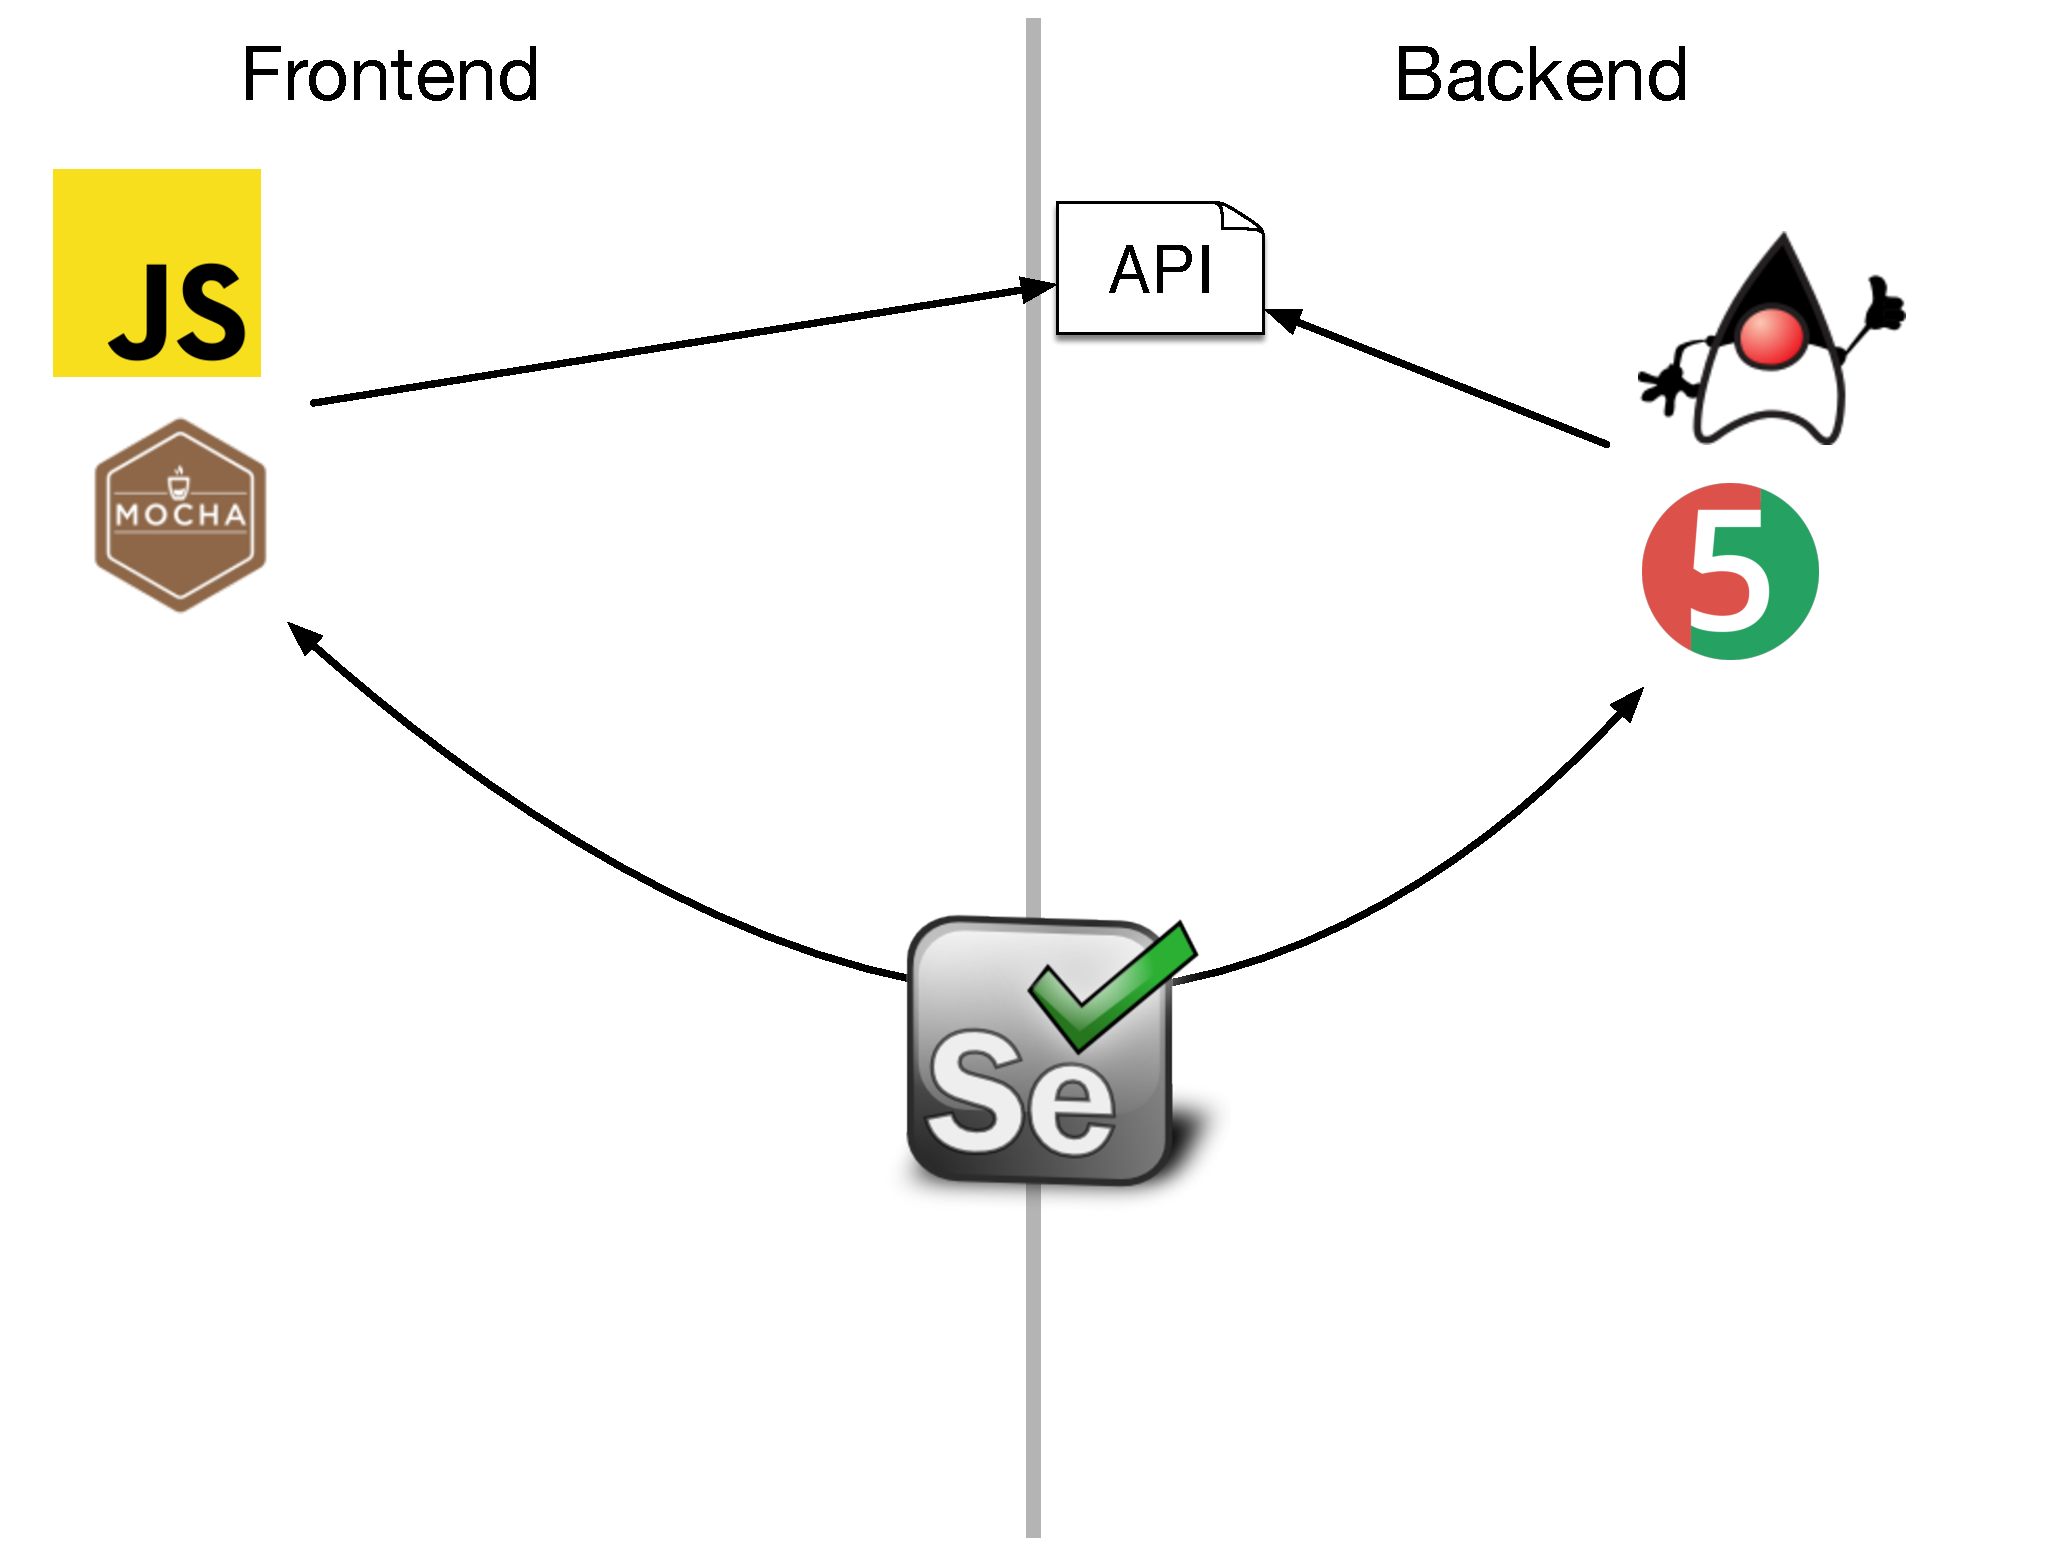
\includegraphics[width=\textwidth]{images/super-naive-approach-4.pdf}
}

\only<2>{
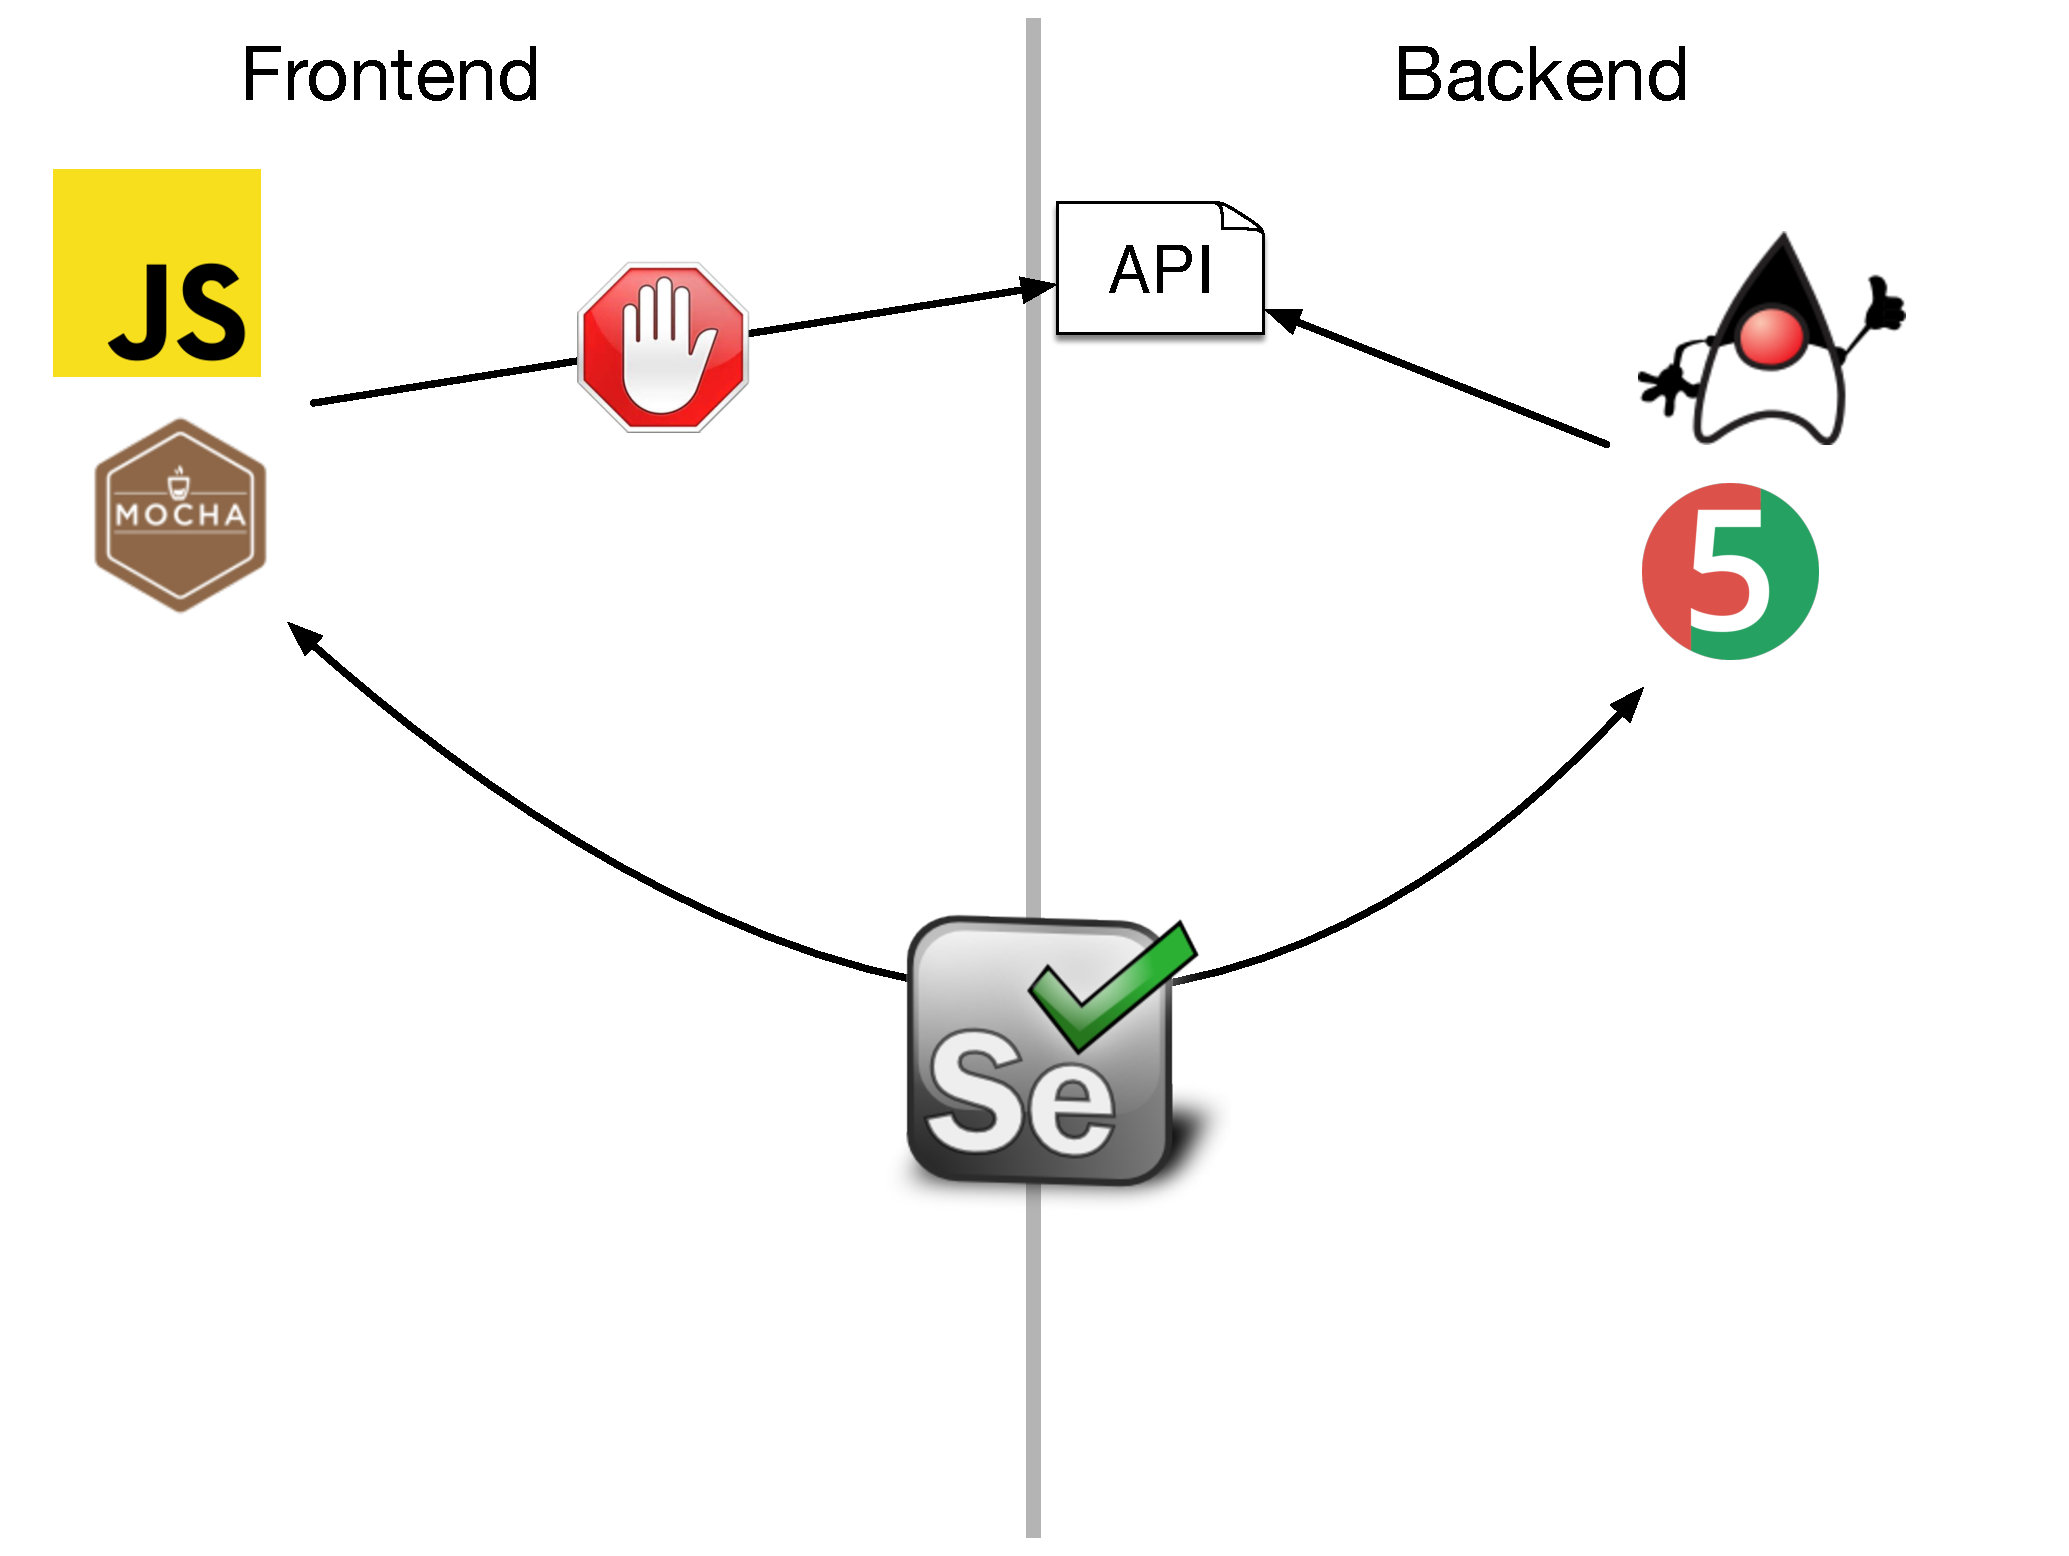
\includegraphics[width=\textwidth]{images/super-naive-approach-5.pdf}
}

\only<3>{
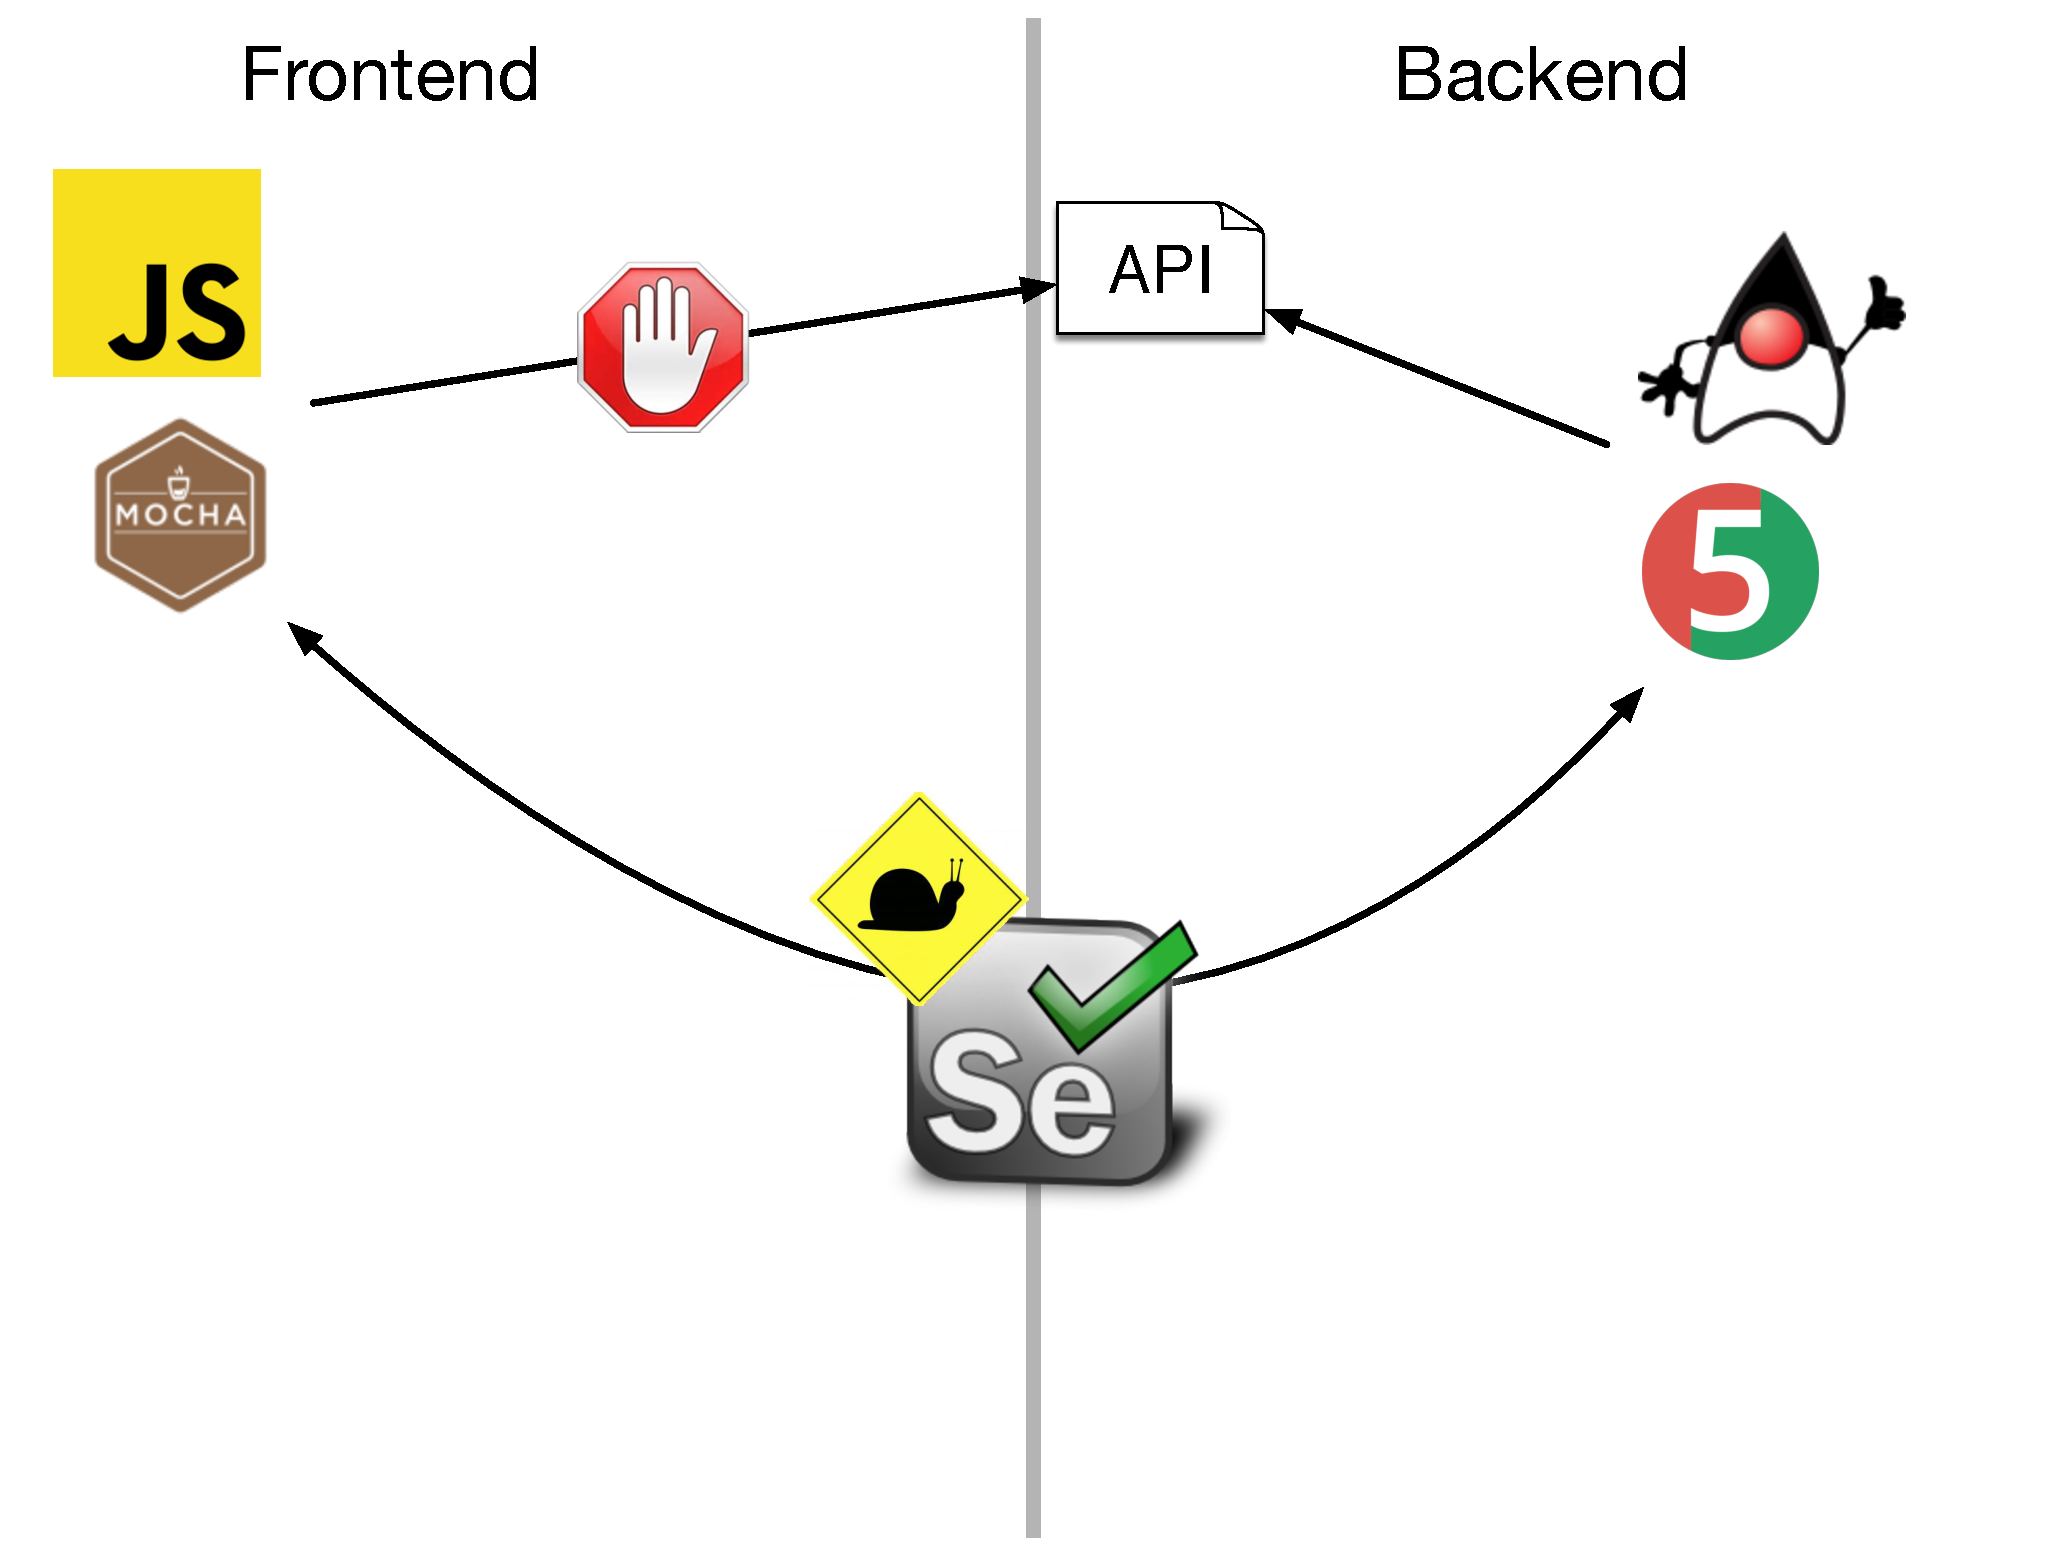
\includegraphics[width=\textwidth]{images/super-naive-approach-6.pdf}
}

\only<4>{
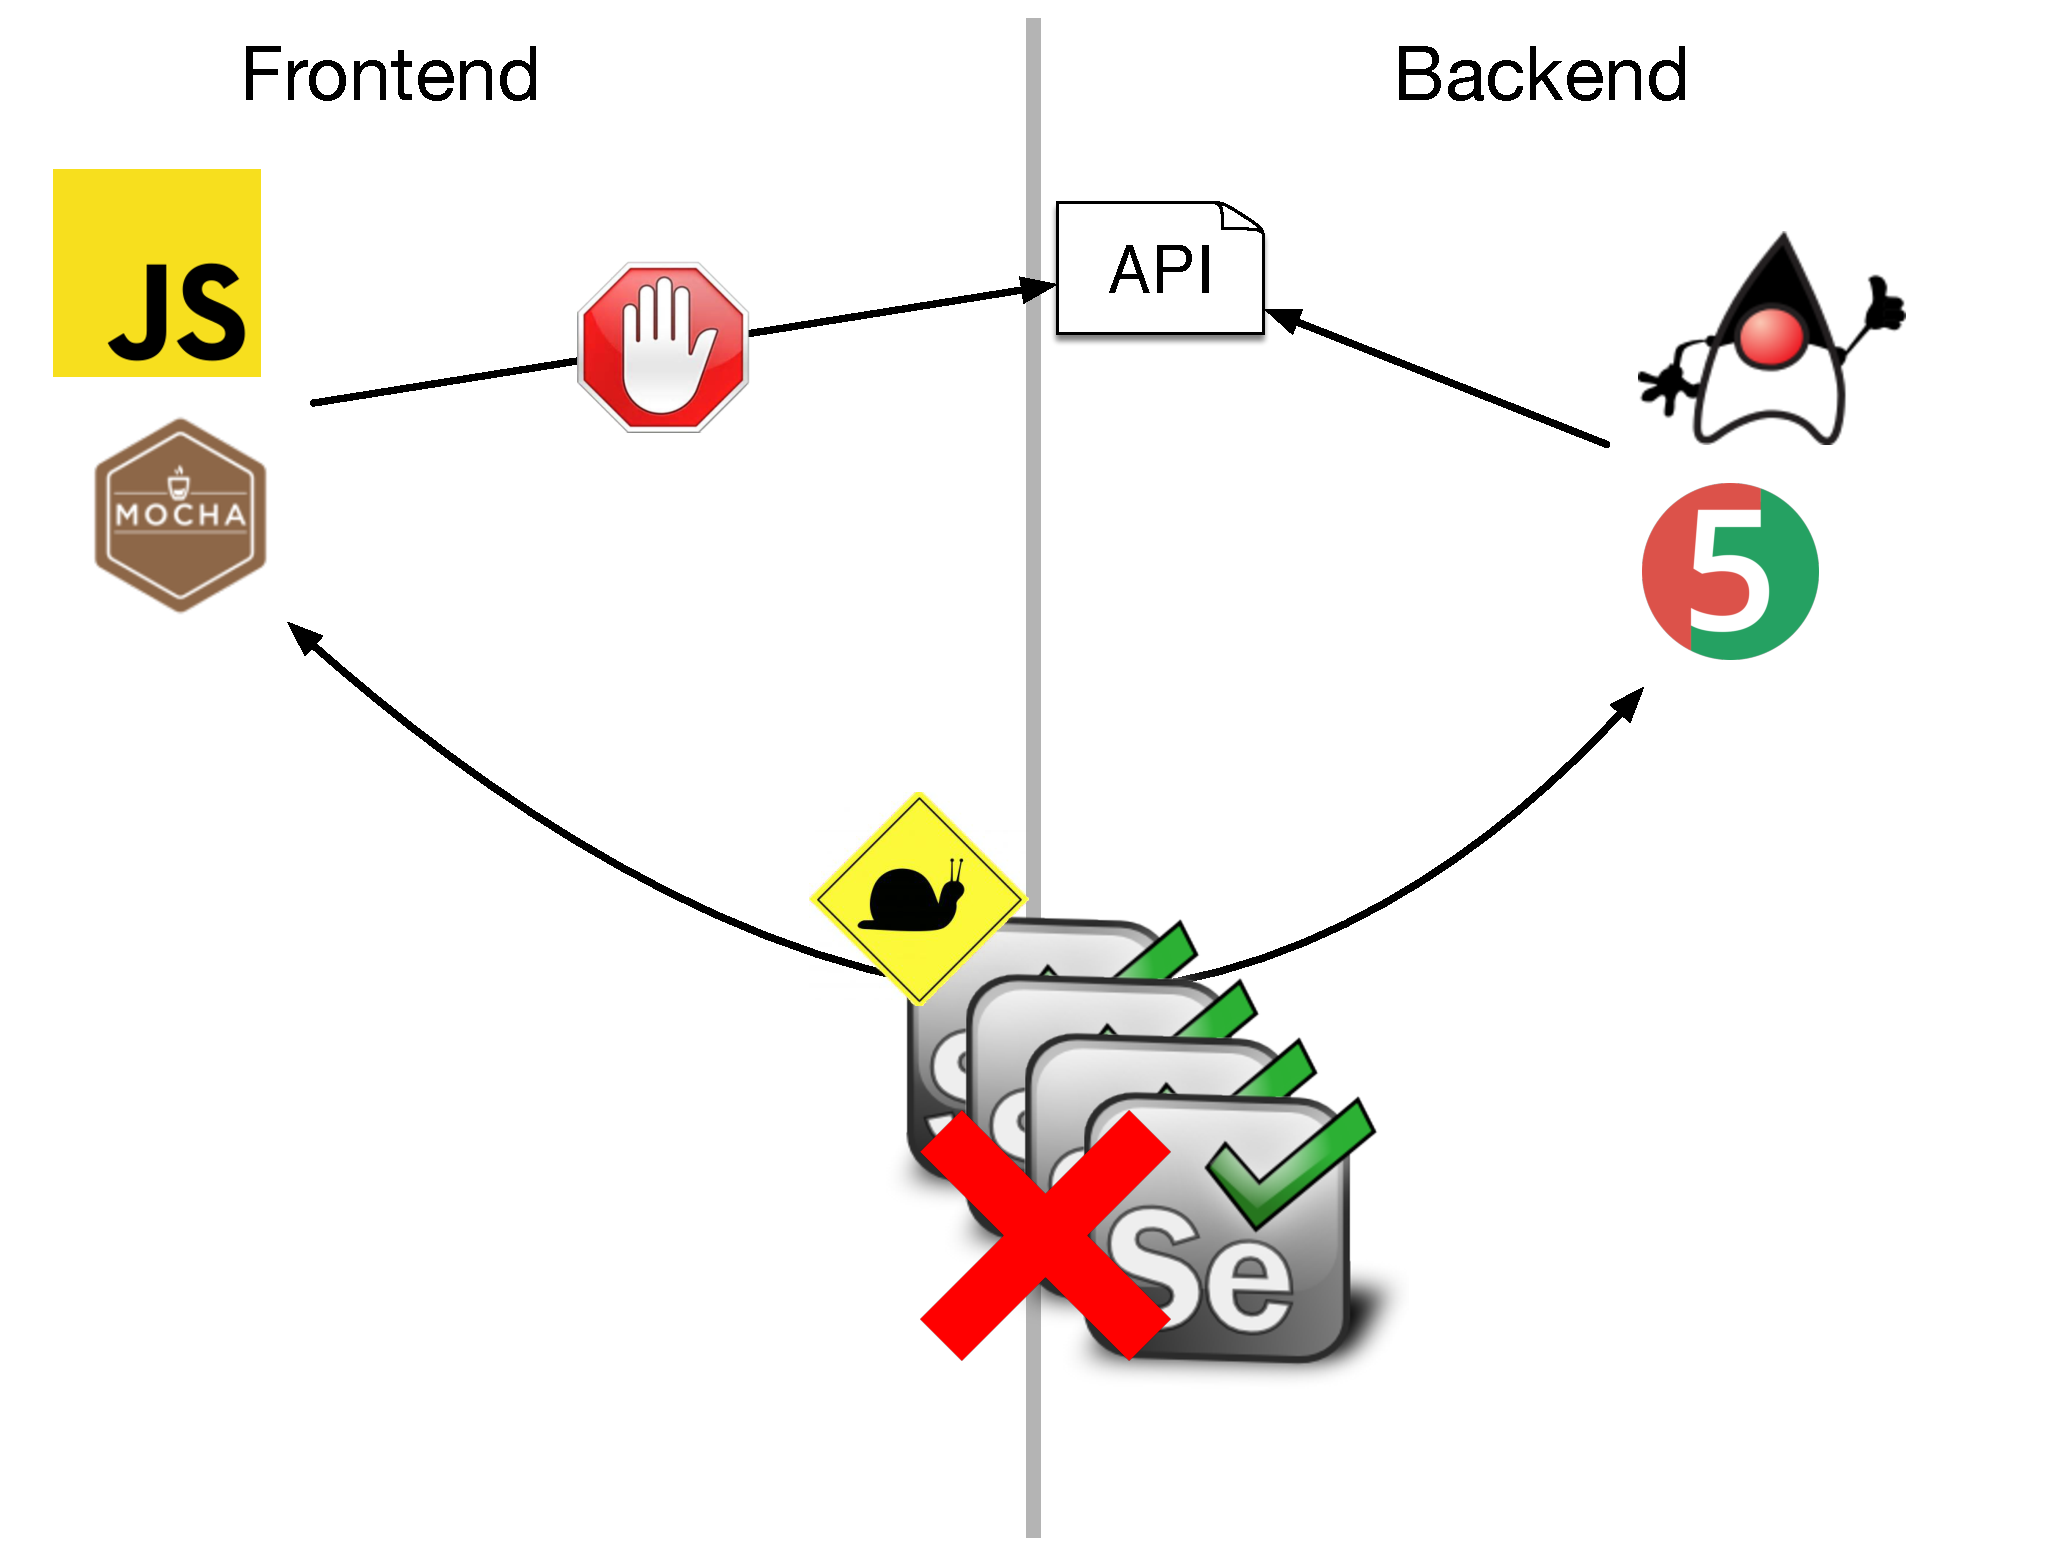
\includegraphics[width=\textwidth]{images/super-naive-approach-7.pdf}
}

\end{frame}


%%%%%%%%%%%%%%%%%%%%%%%%%%%%%%%%%%%%%%%%%%%%%%%%%%
\begin{frame}[fragile]{}

\begin{center}
{\Huge
``Still Quite Na\"ive'' Approach
}
\end{center}

\end{frame}

\begin{frame}[fragile]{}

\only<1>{
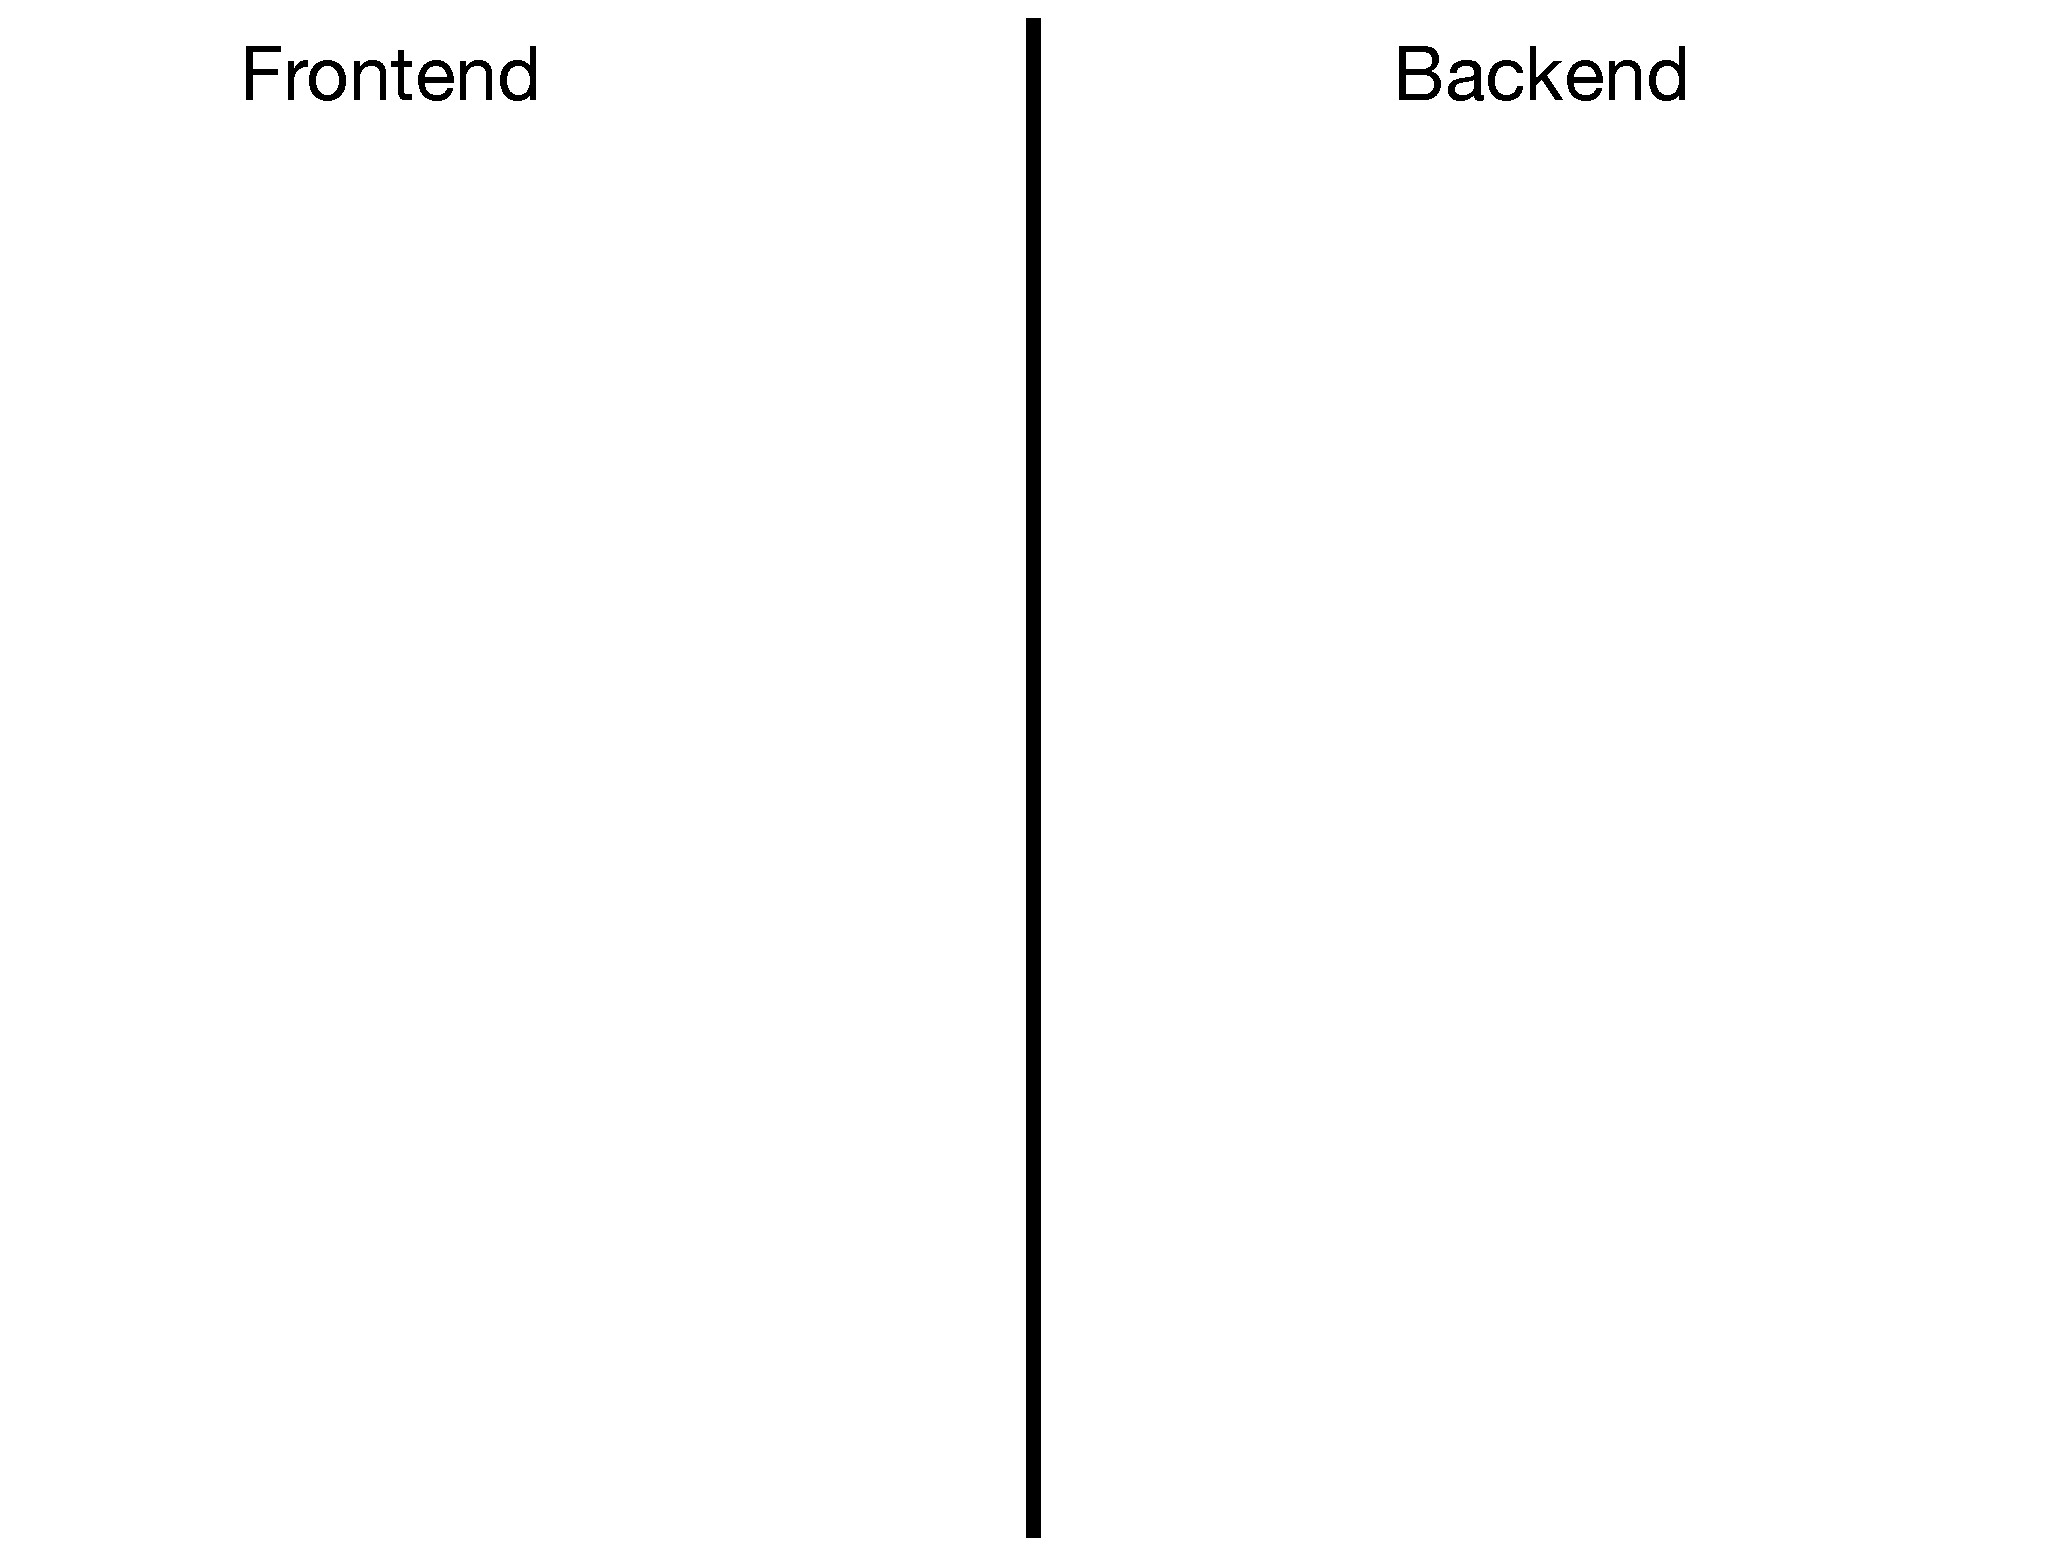
\includegraphics[width=\textwidth]{images/still-quite-naive-approach-0.pdf}
}

\only<2>{
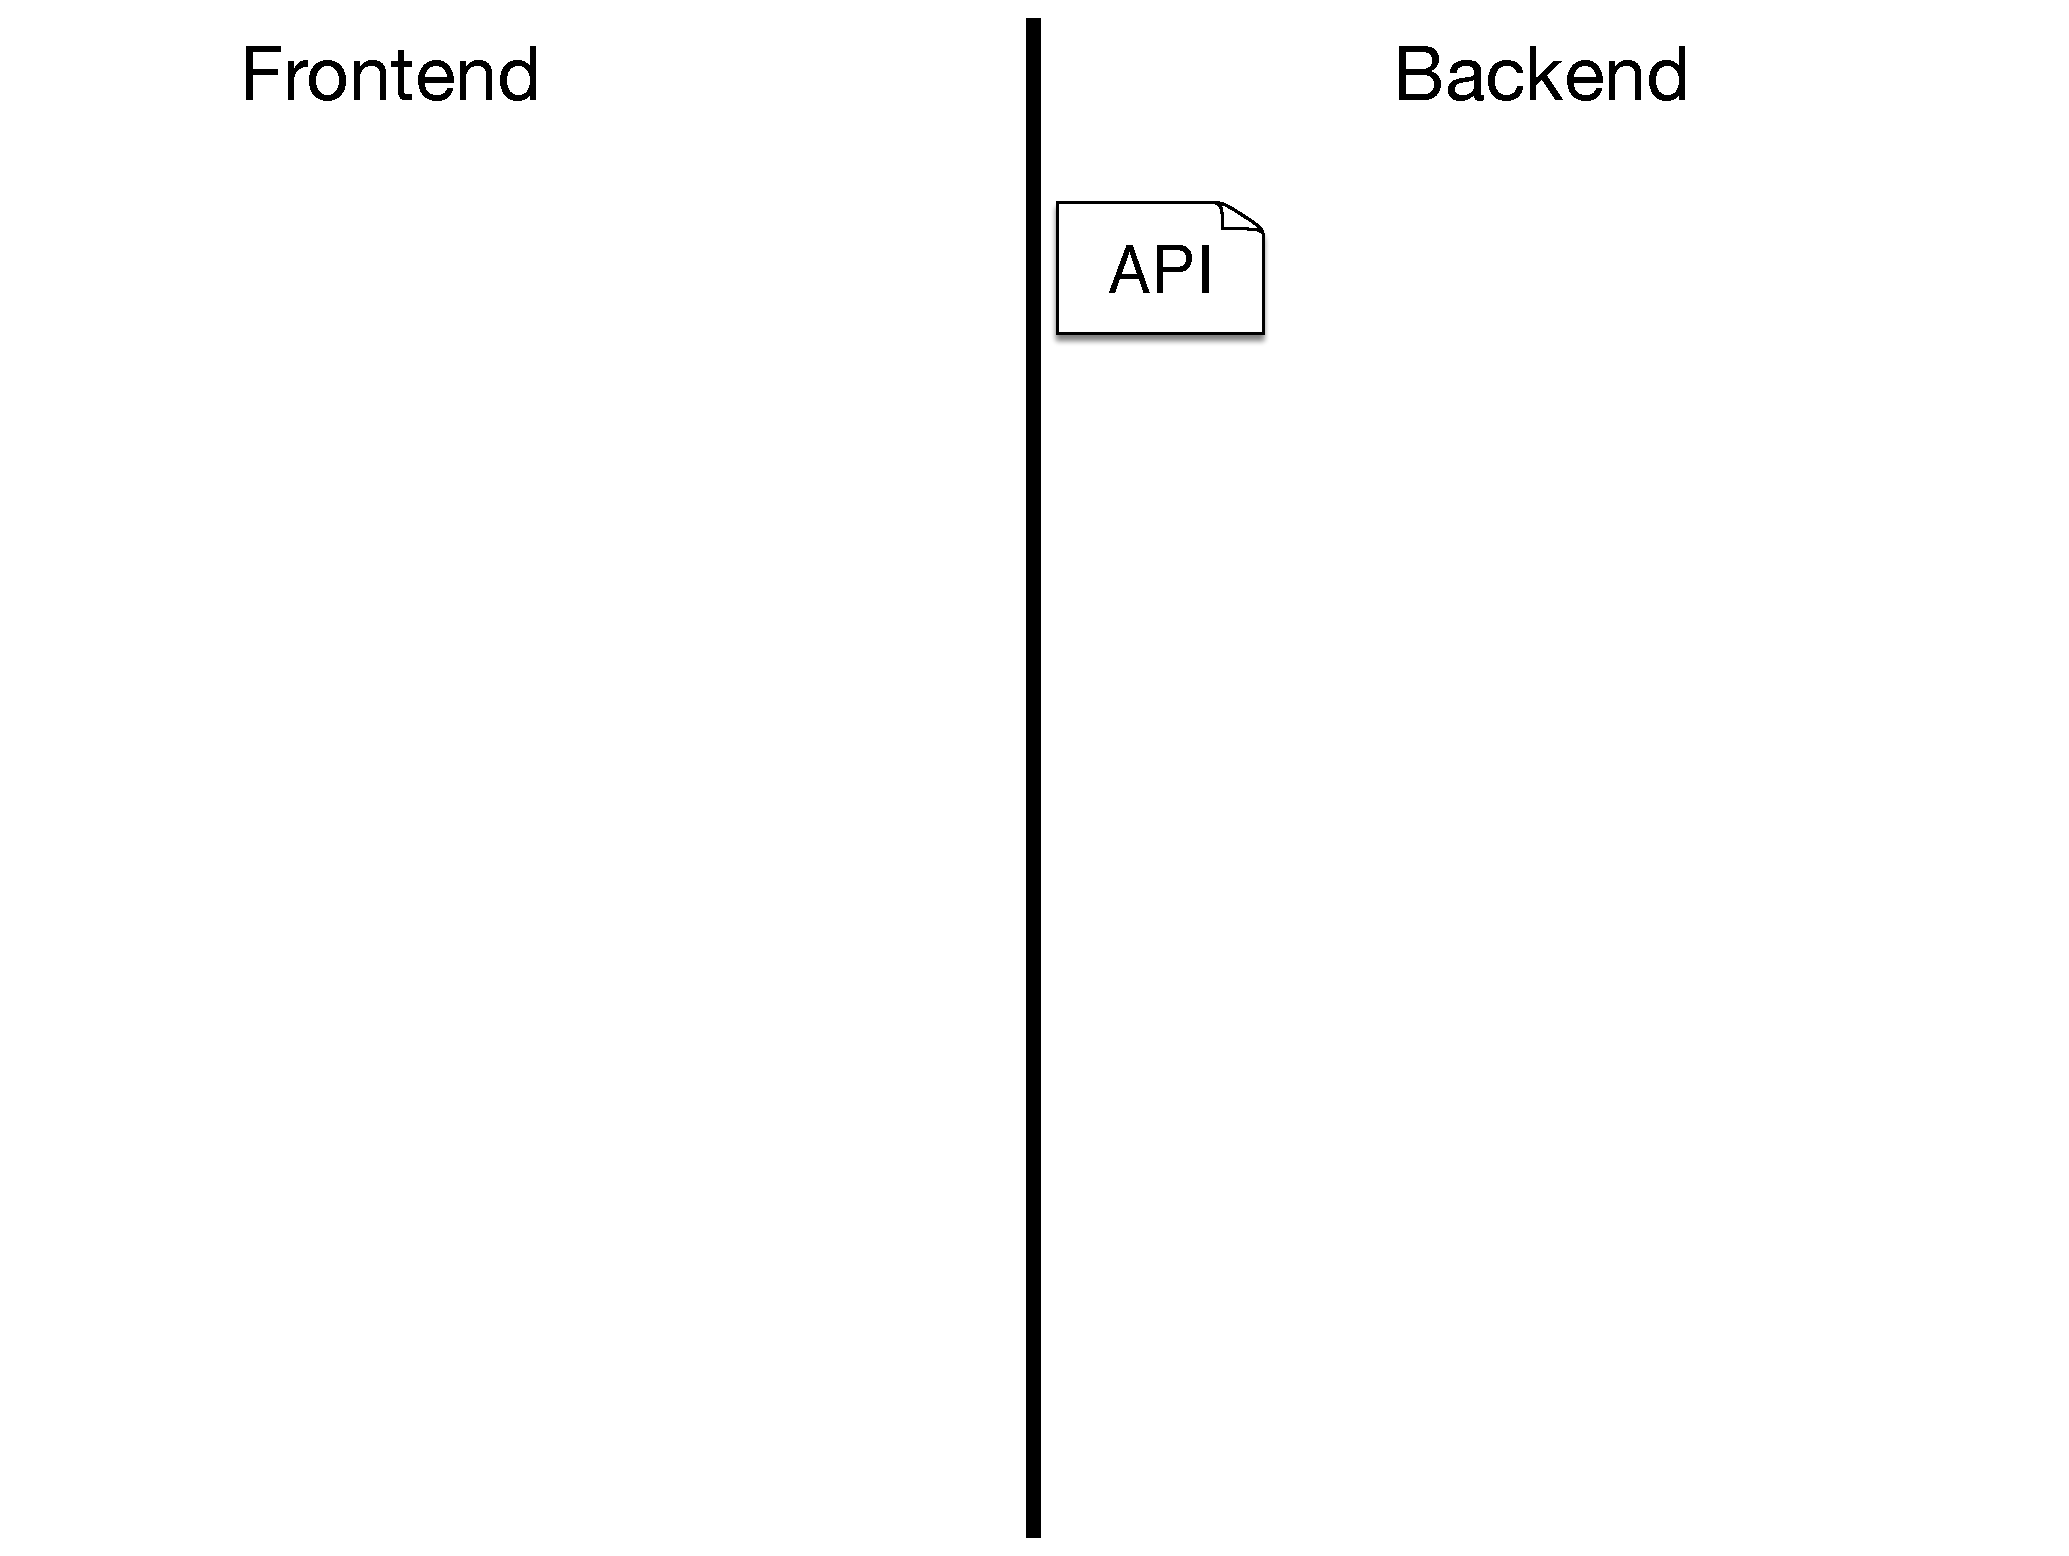
\includegraphics[width=\textwidth]{images/still-quite-naive-approach-1.pdf}
}

\only<3>{
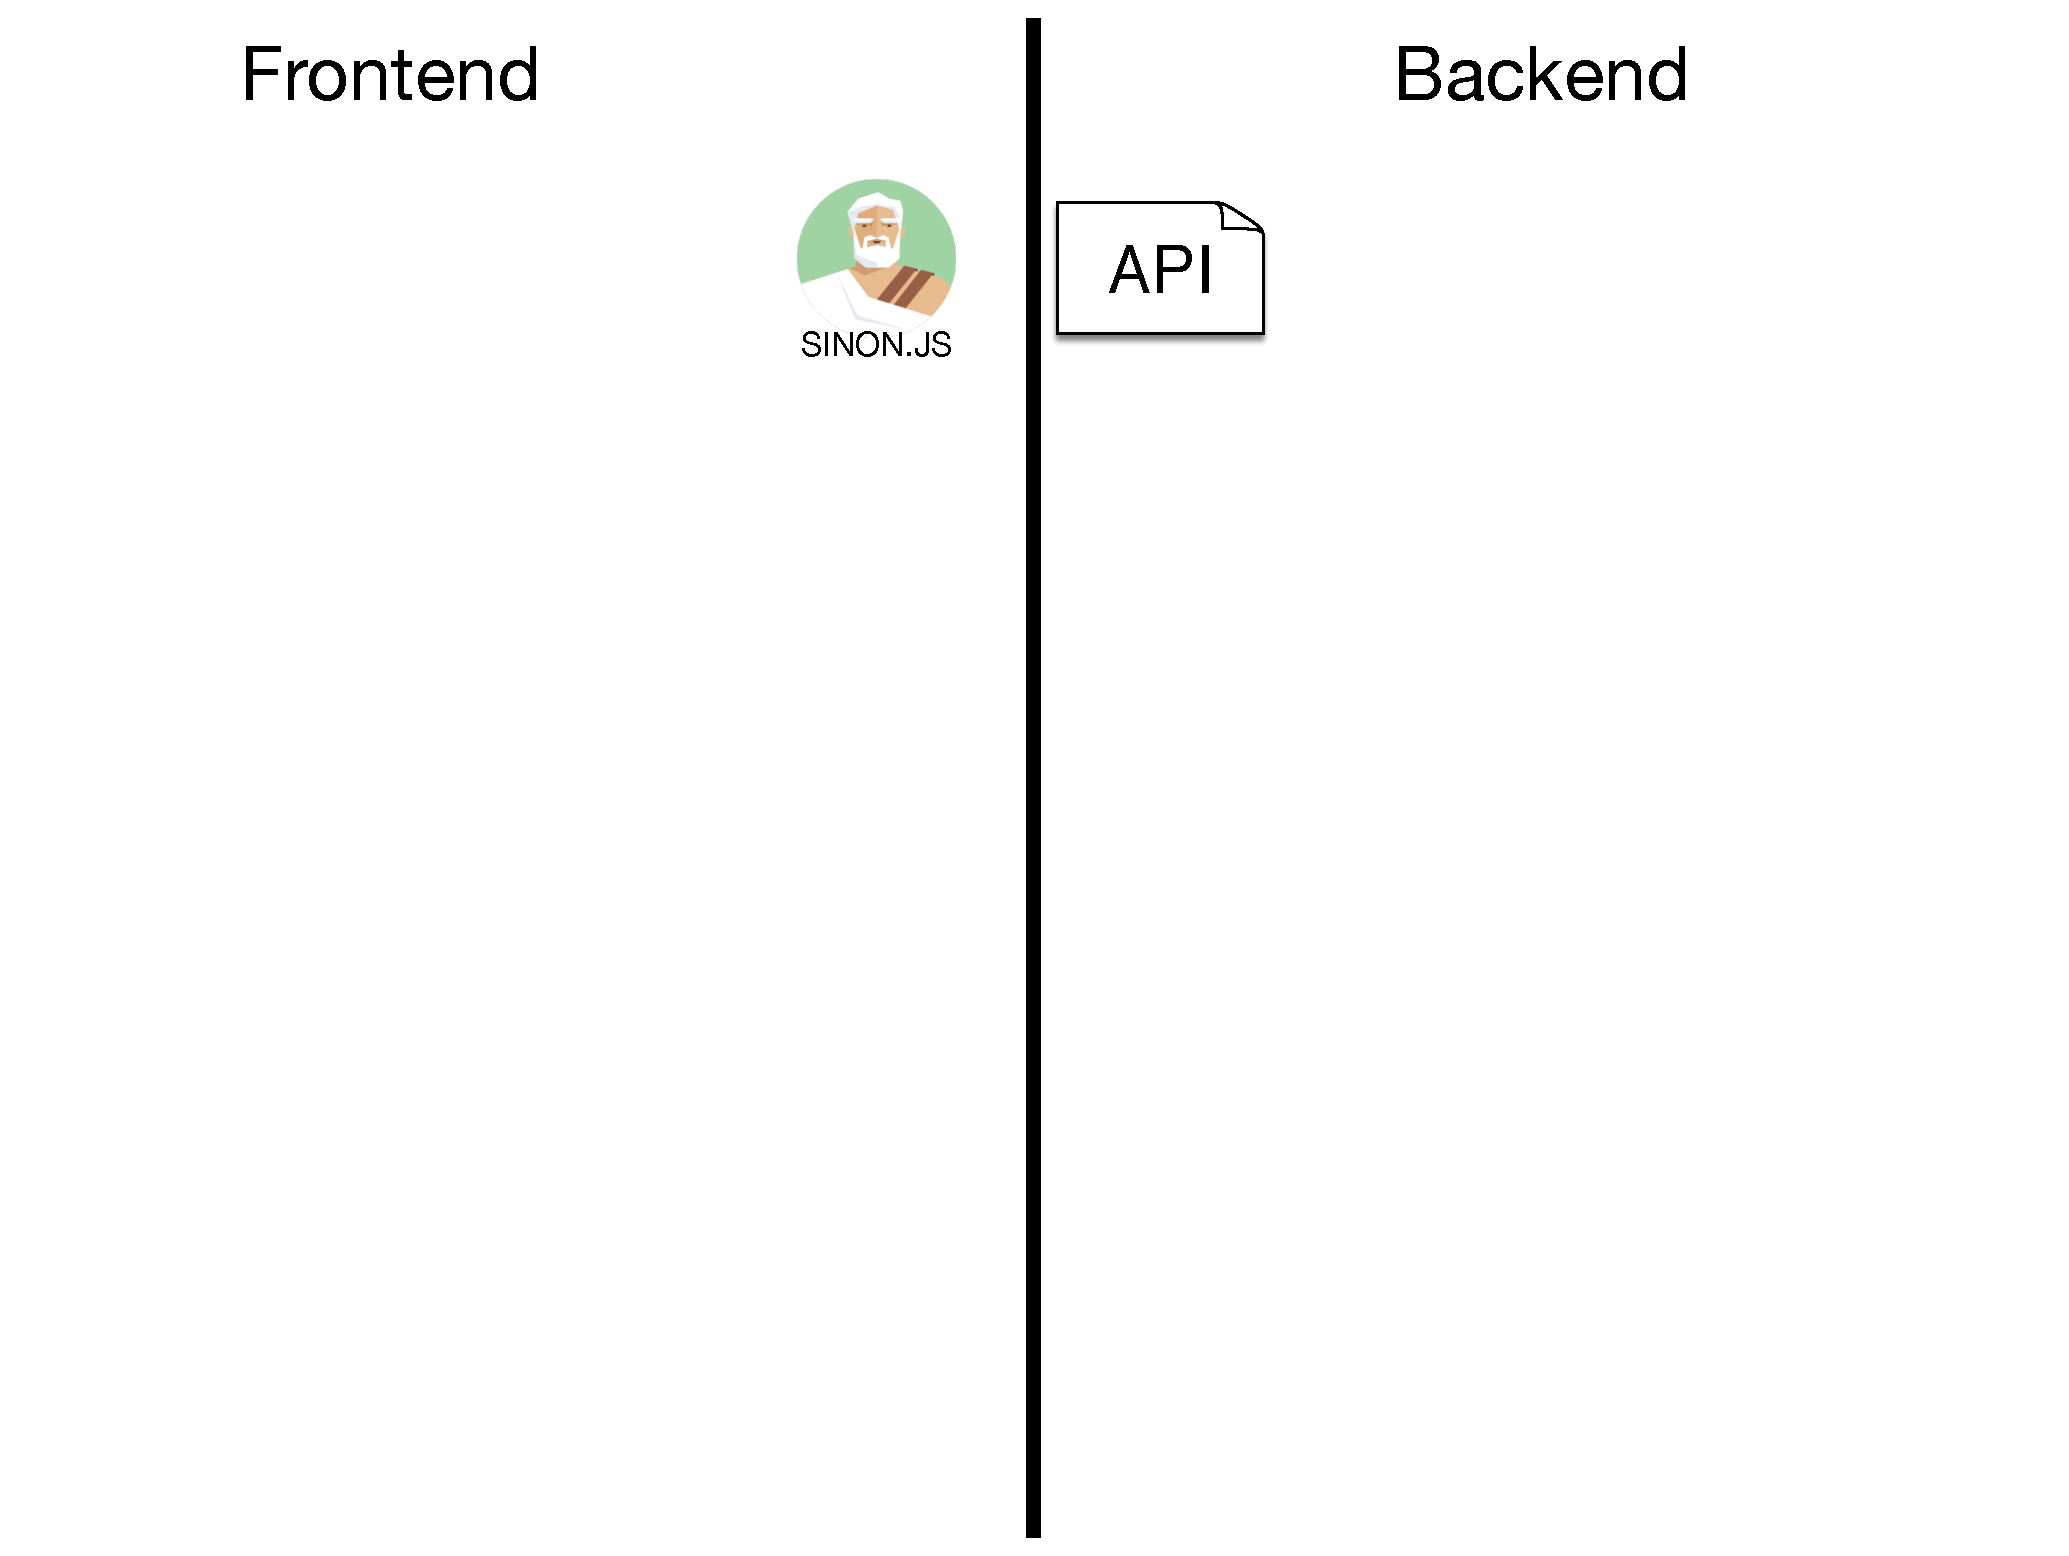
\includegraphics[width=\textwidth]{images/still-quite-naive-approach-2.pdf}
}

\only<4>{
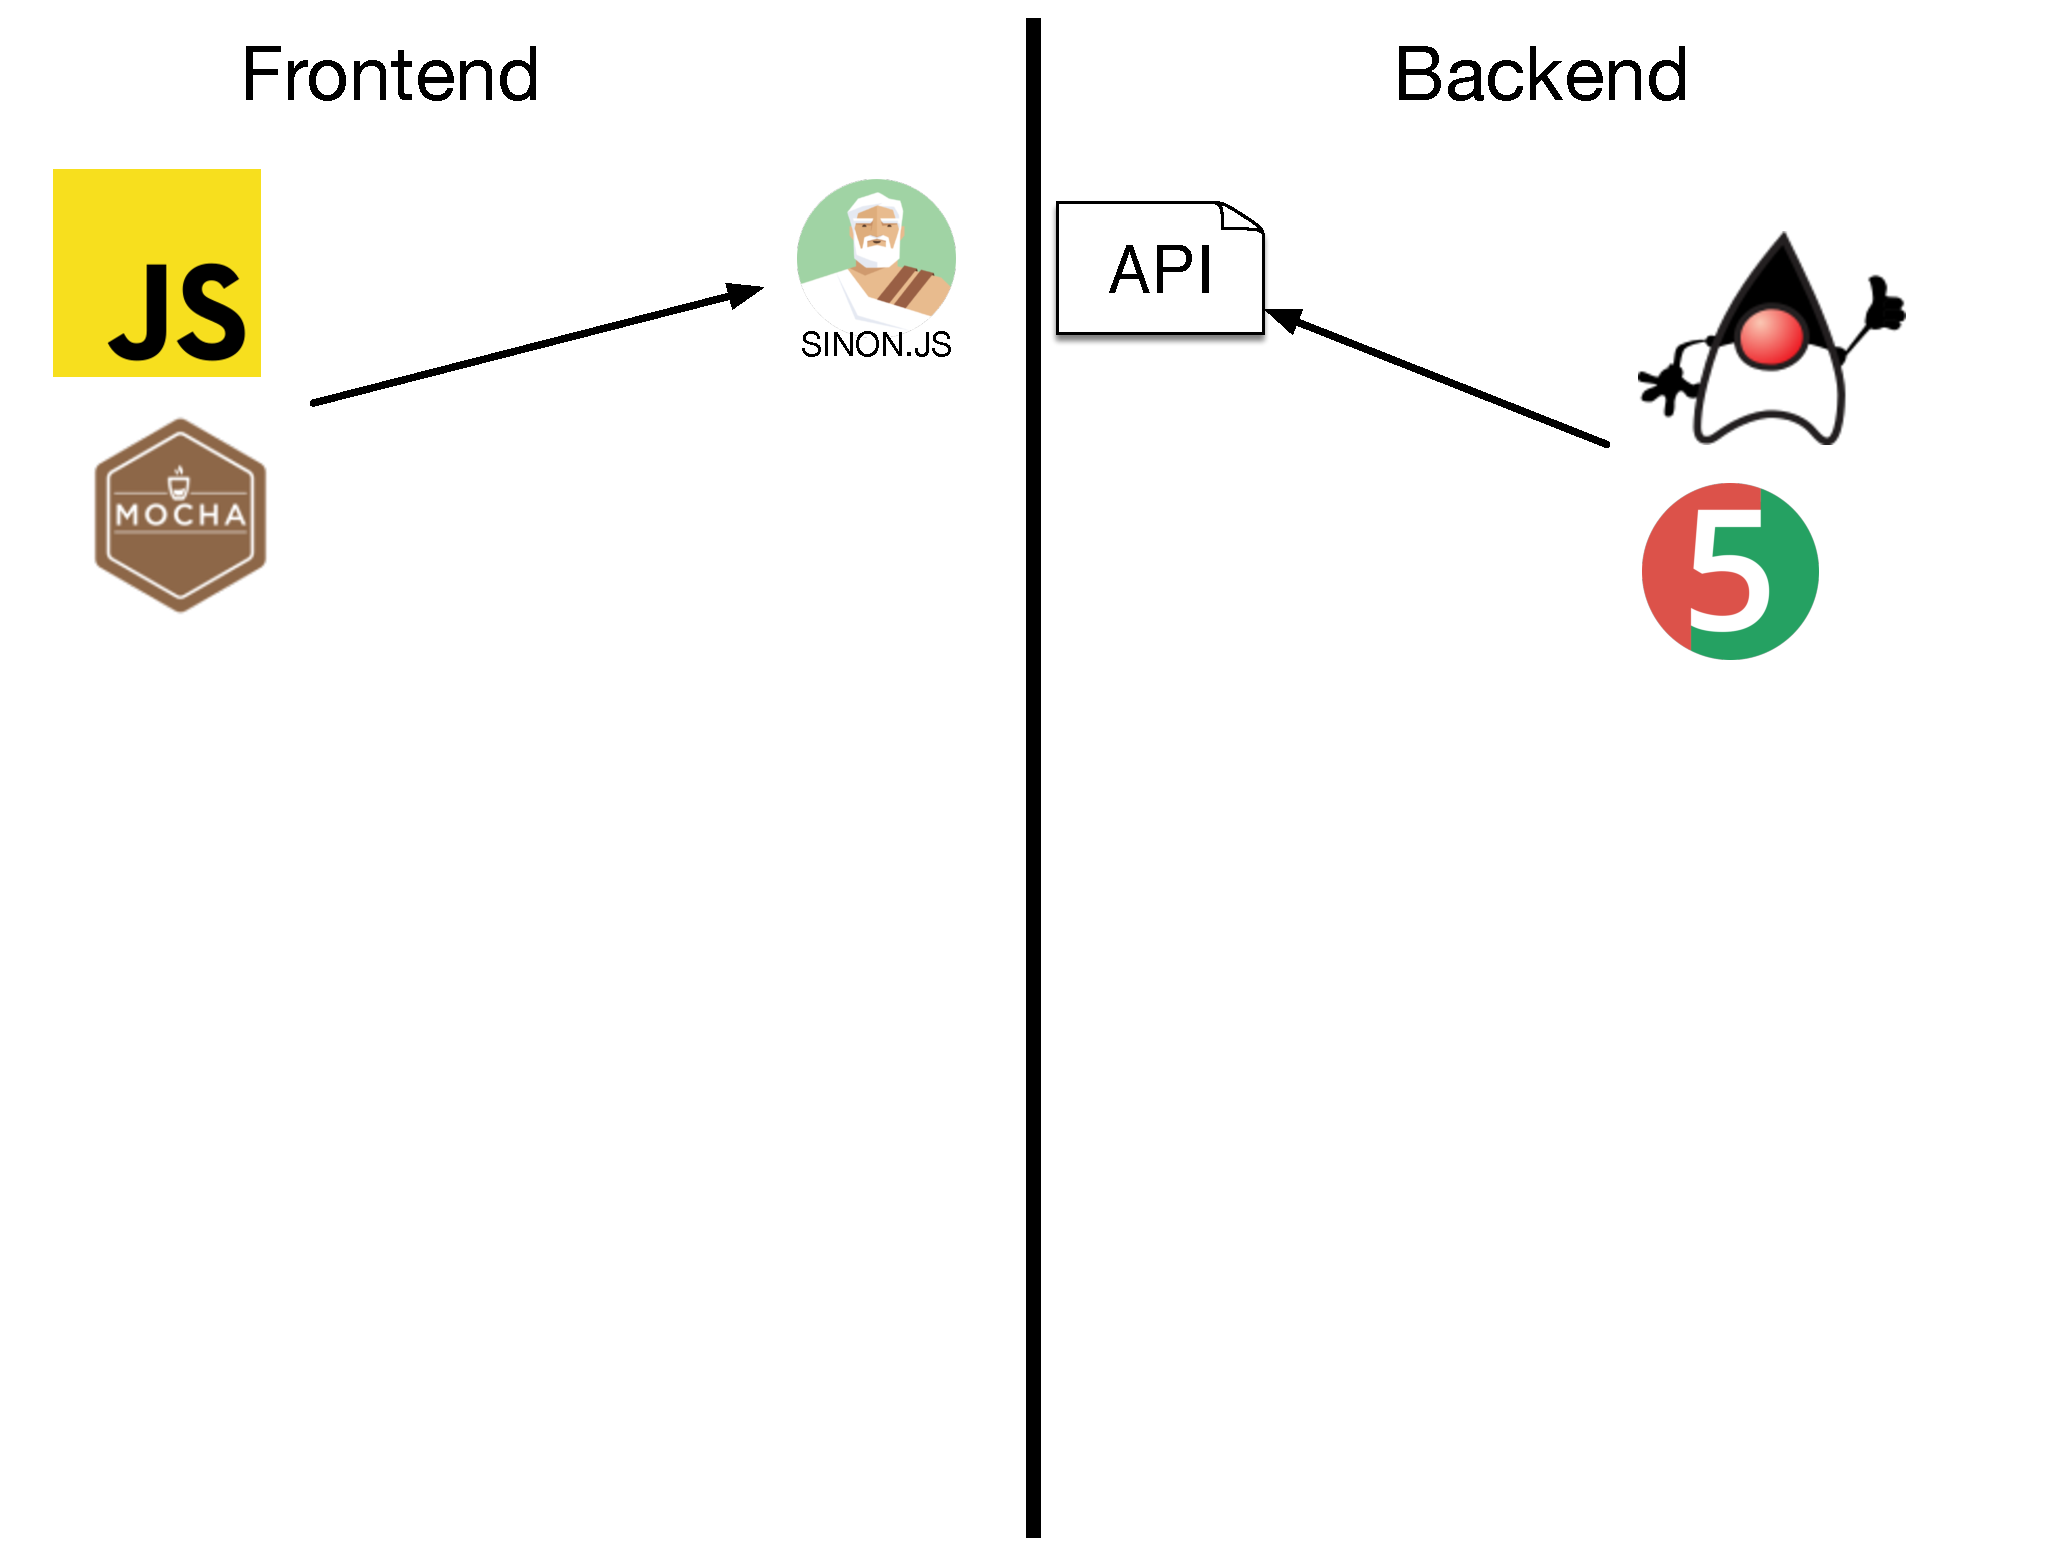
\includegraphics[width=\textwidth]{images/still-quite-naive-approach-3.pdf}
}

\only<5>{
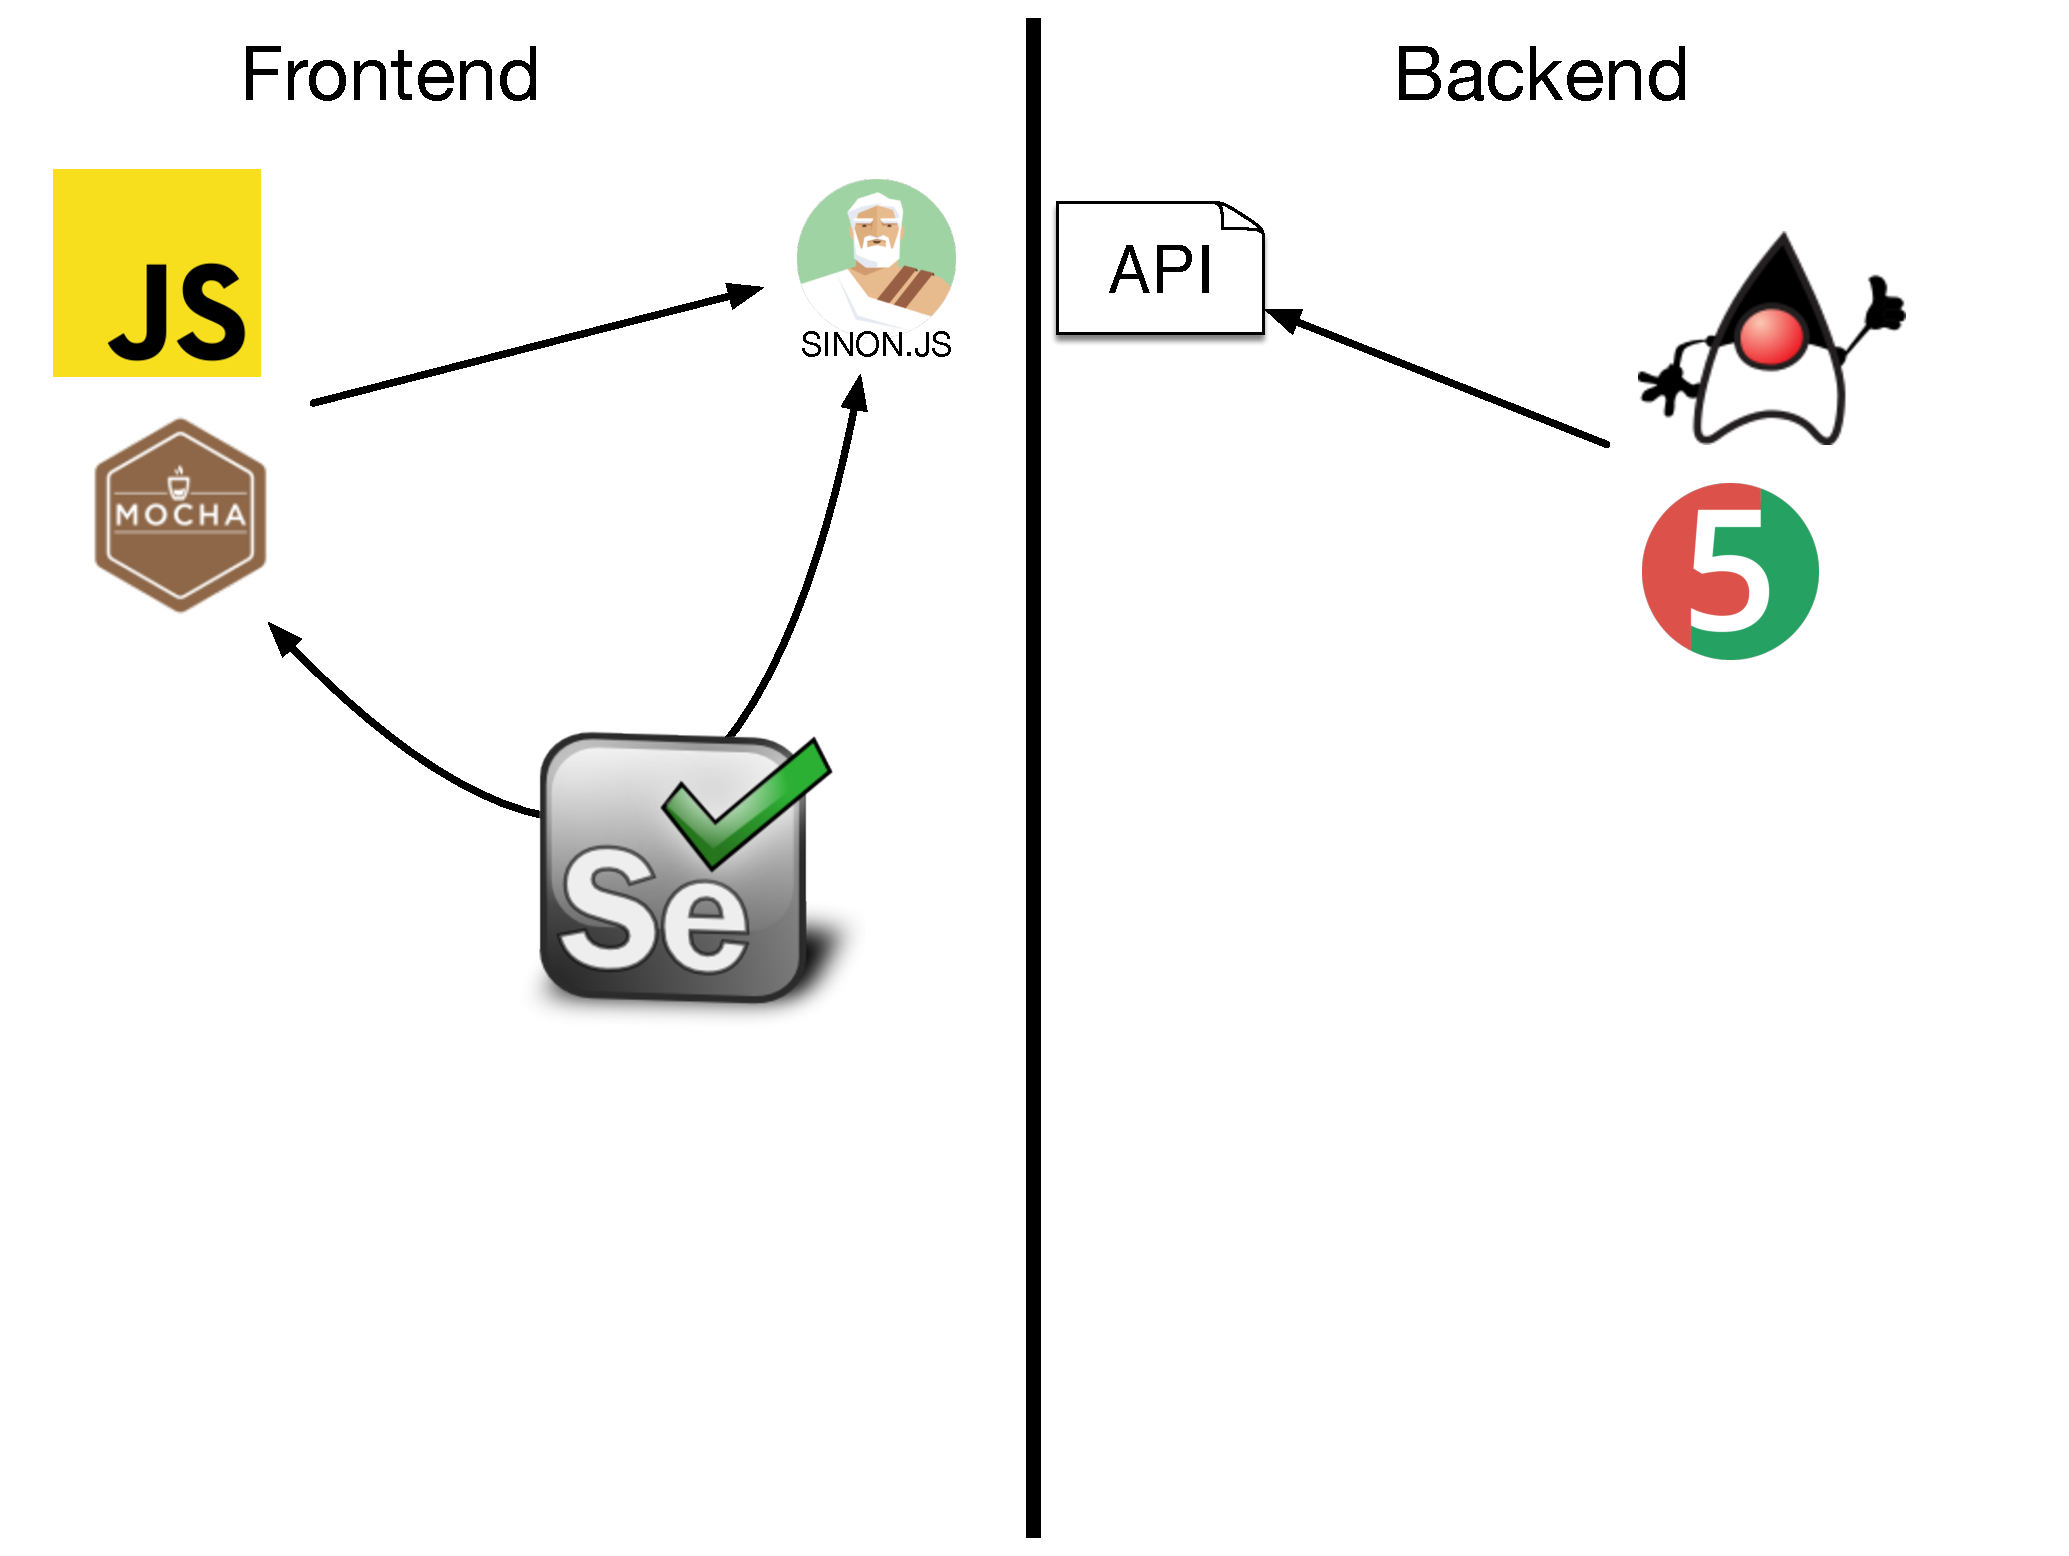
\includegraphics[width=\textwidth]{images/still-quite-naive-approach-4.pdf}
}

\end{frame}

\begin{frame}[fragile]{}

\begin{center}
{\Huge
But $\ldots$
}
\end{center}

\end{frame}

\begin{frame}[fragile]{}

\only<1>{
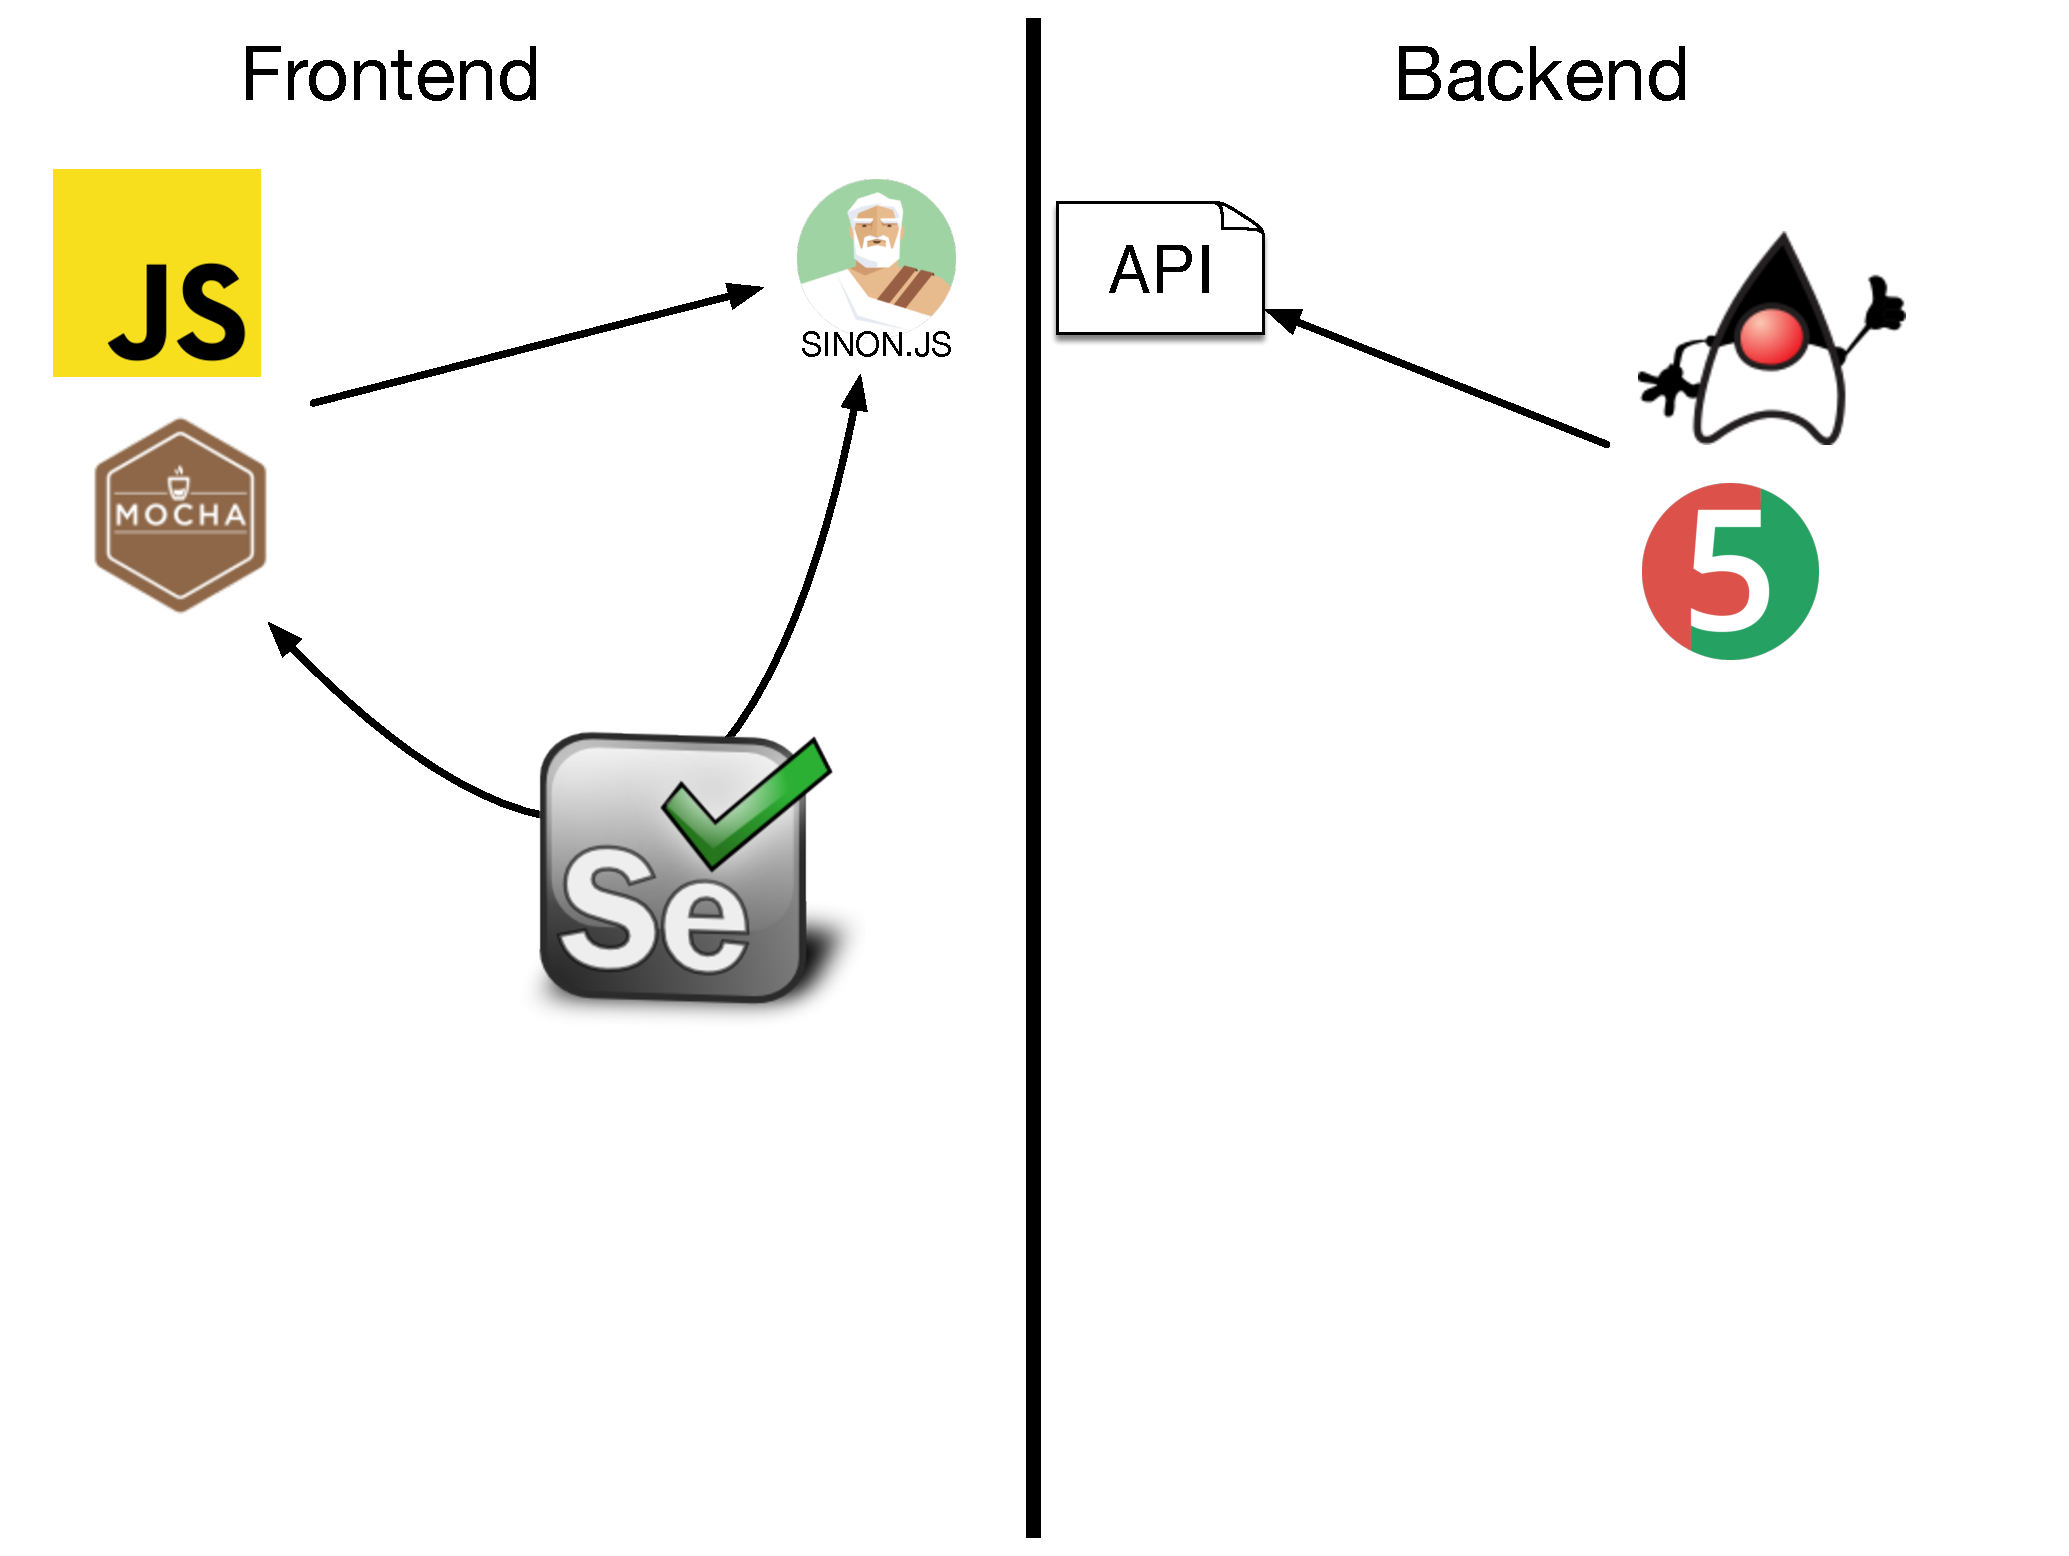
\includegraphics[width=\textwidth]{images/still-quite-naive-approach-4.pdf}
}

\only<2>{
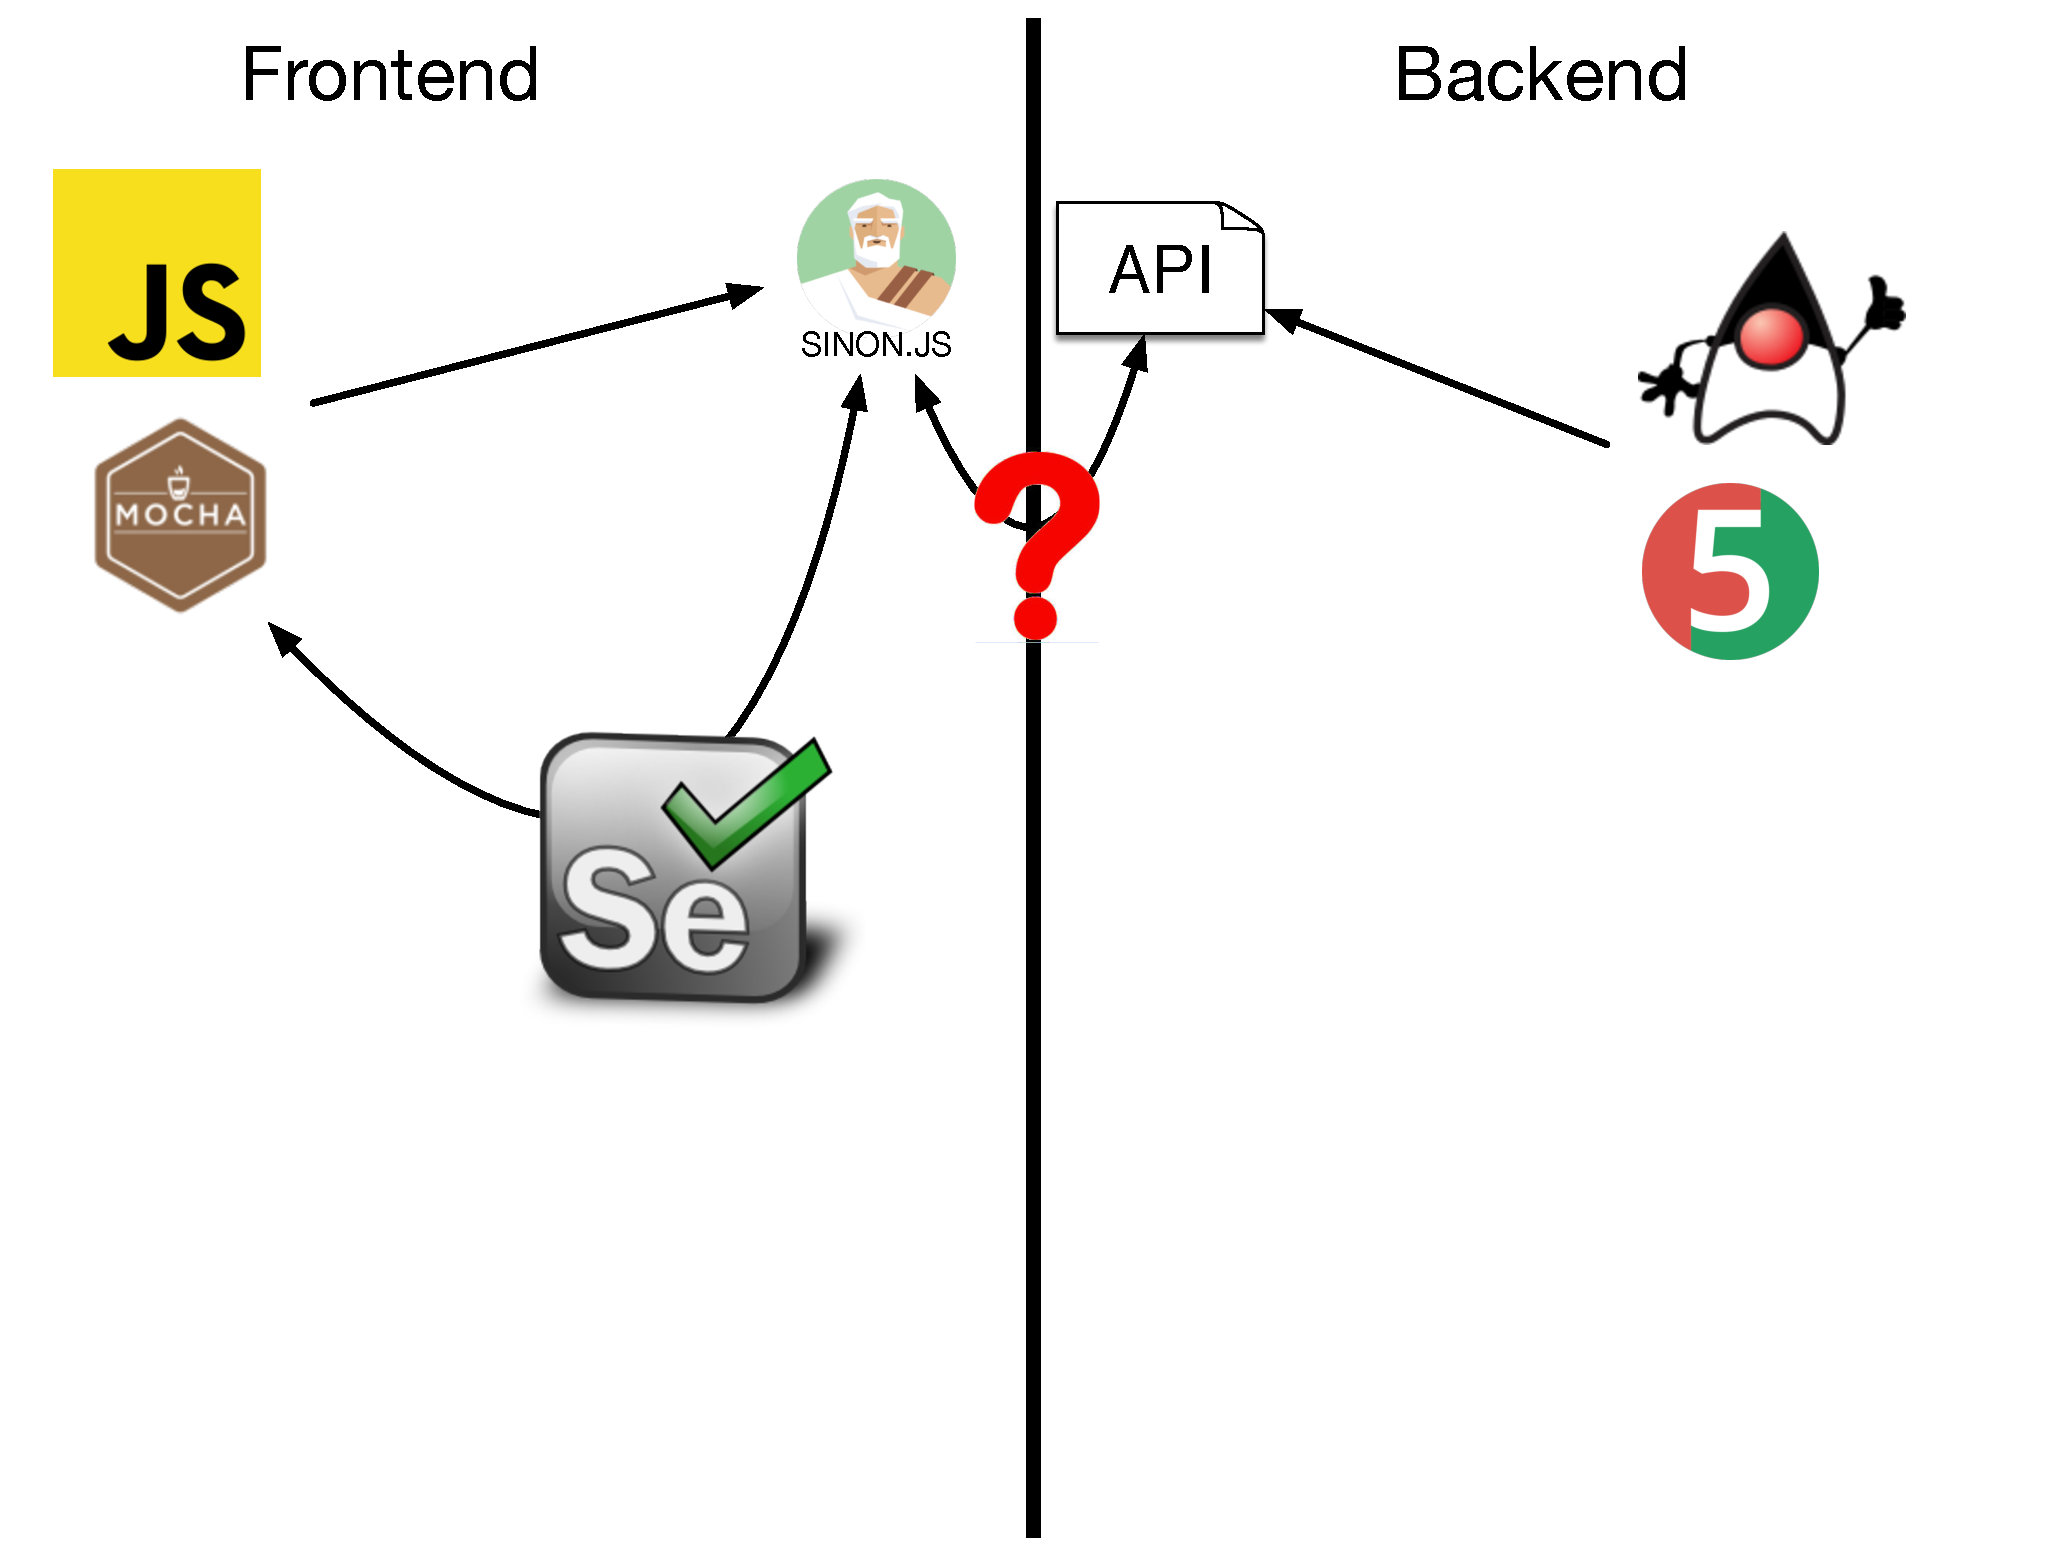
\includegraphics[width=\textwidth]{images/still-quite-naive-approach-5.pdf}
}

\only<3>{
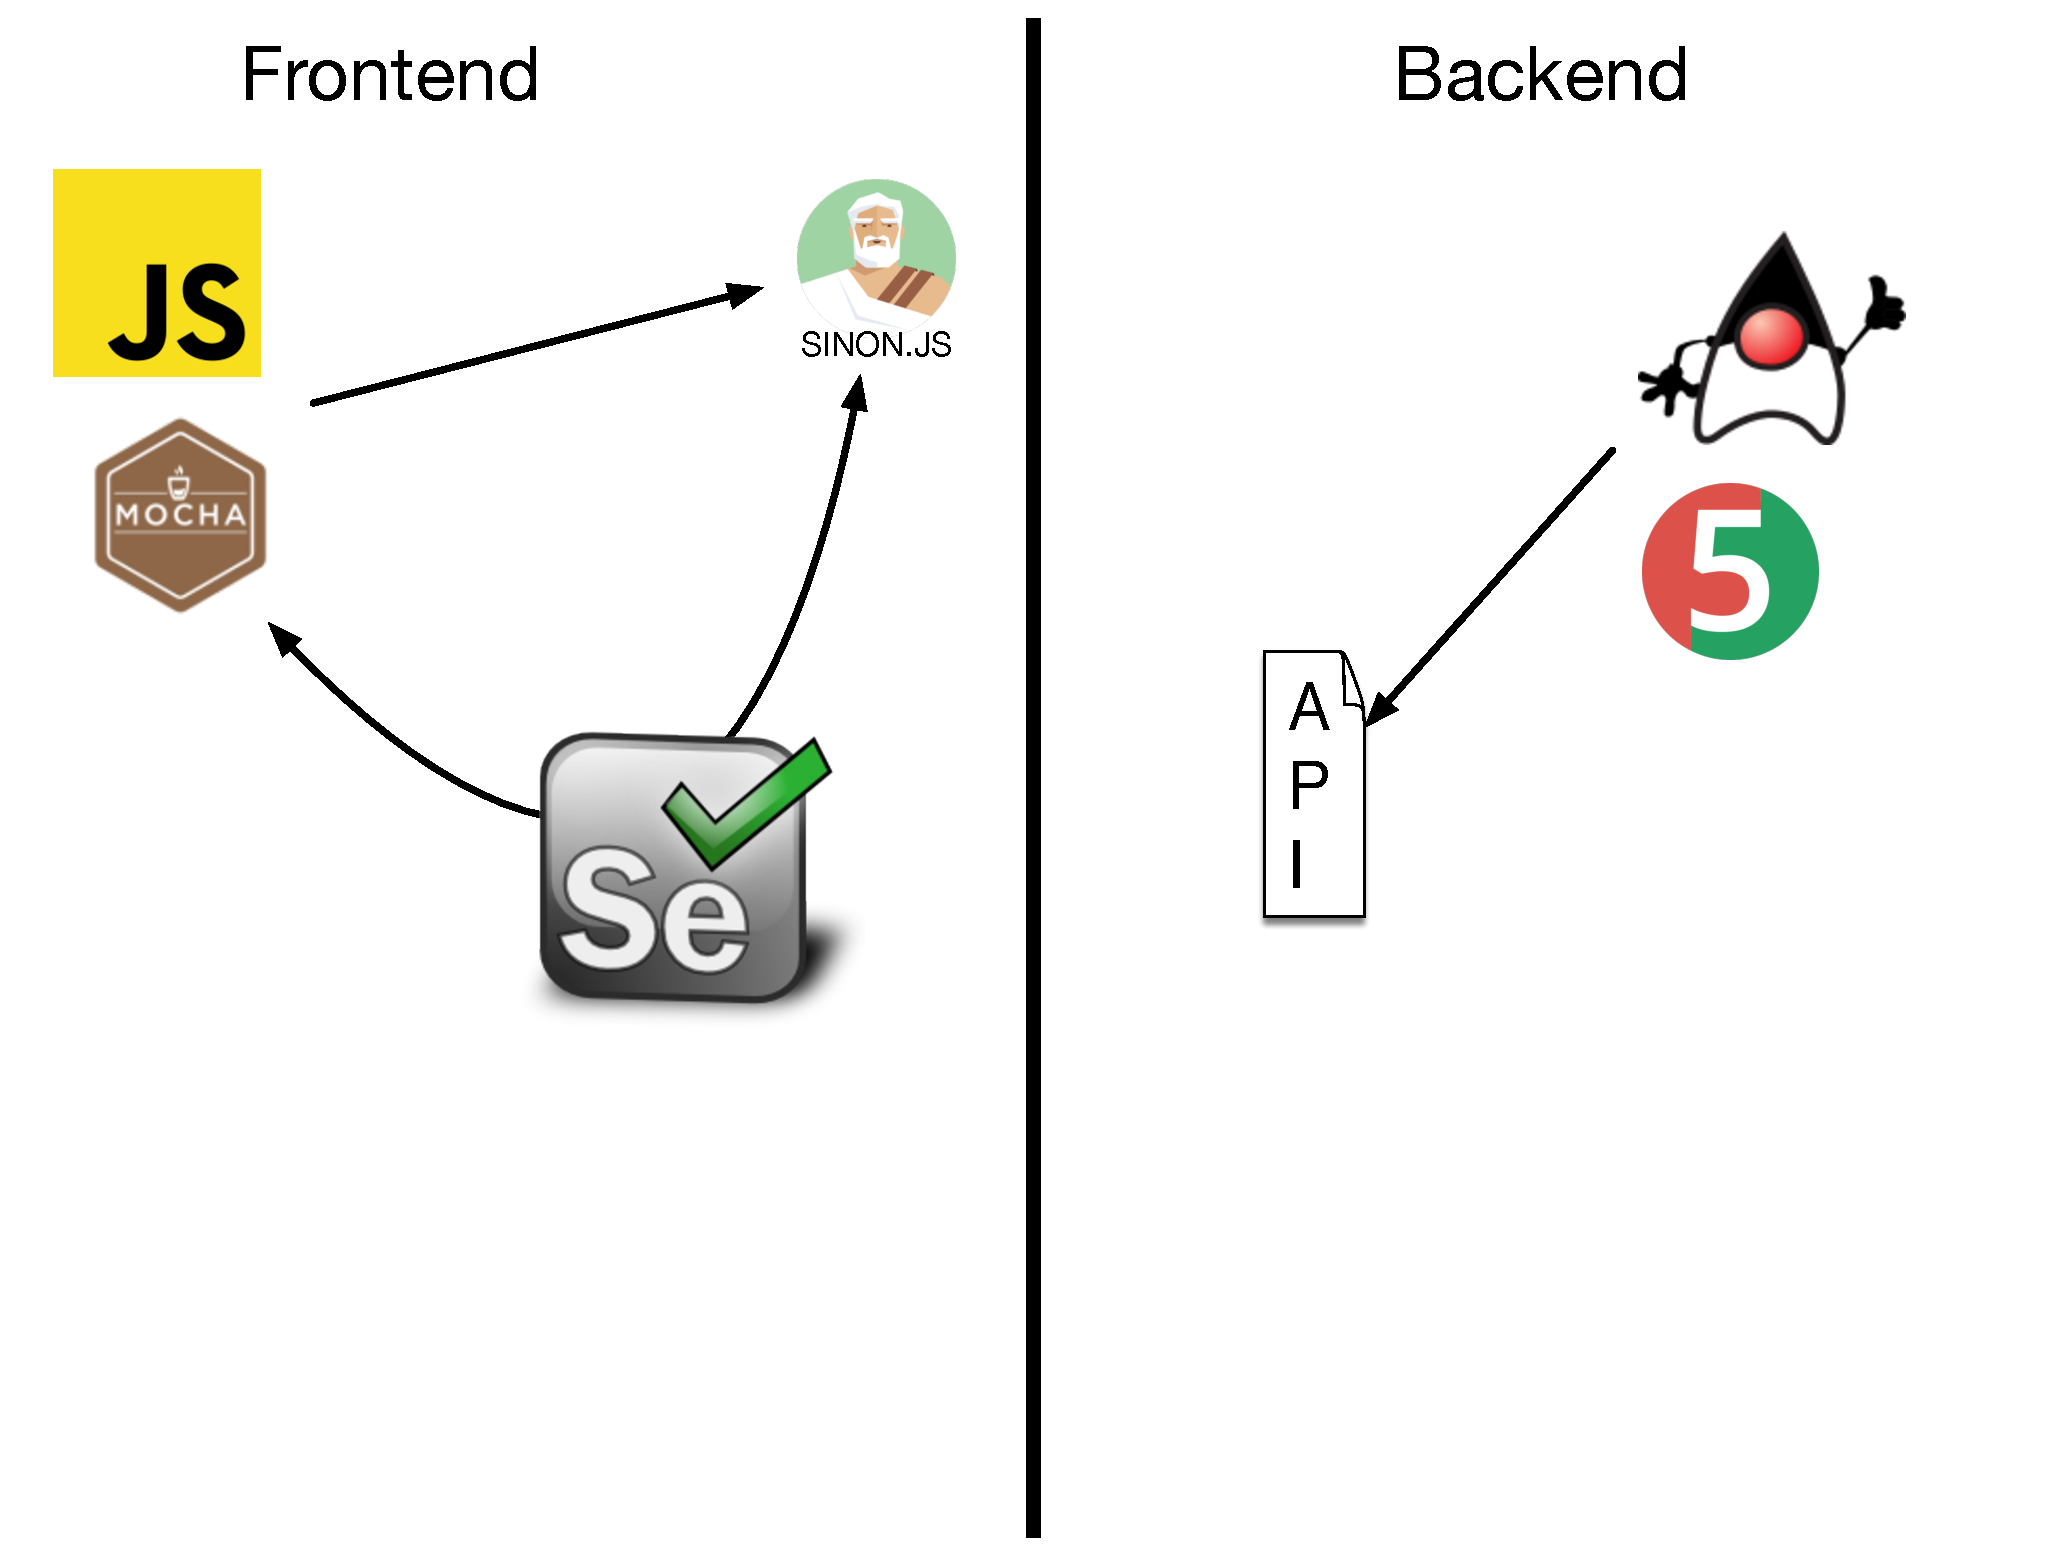
\includegraphics[width=\textwidth]{images/still-quite-naive-approach-6.pdf}
}

\only<4>{
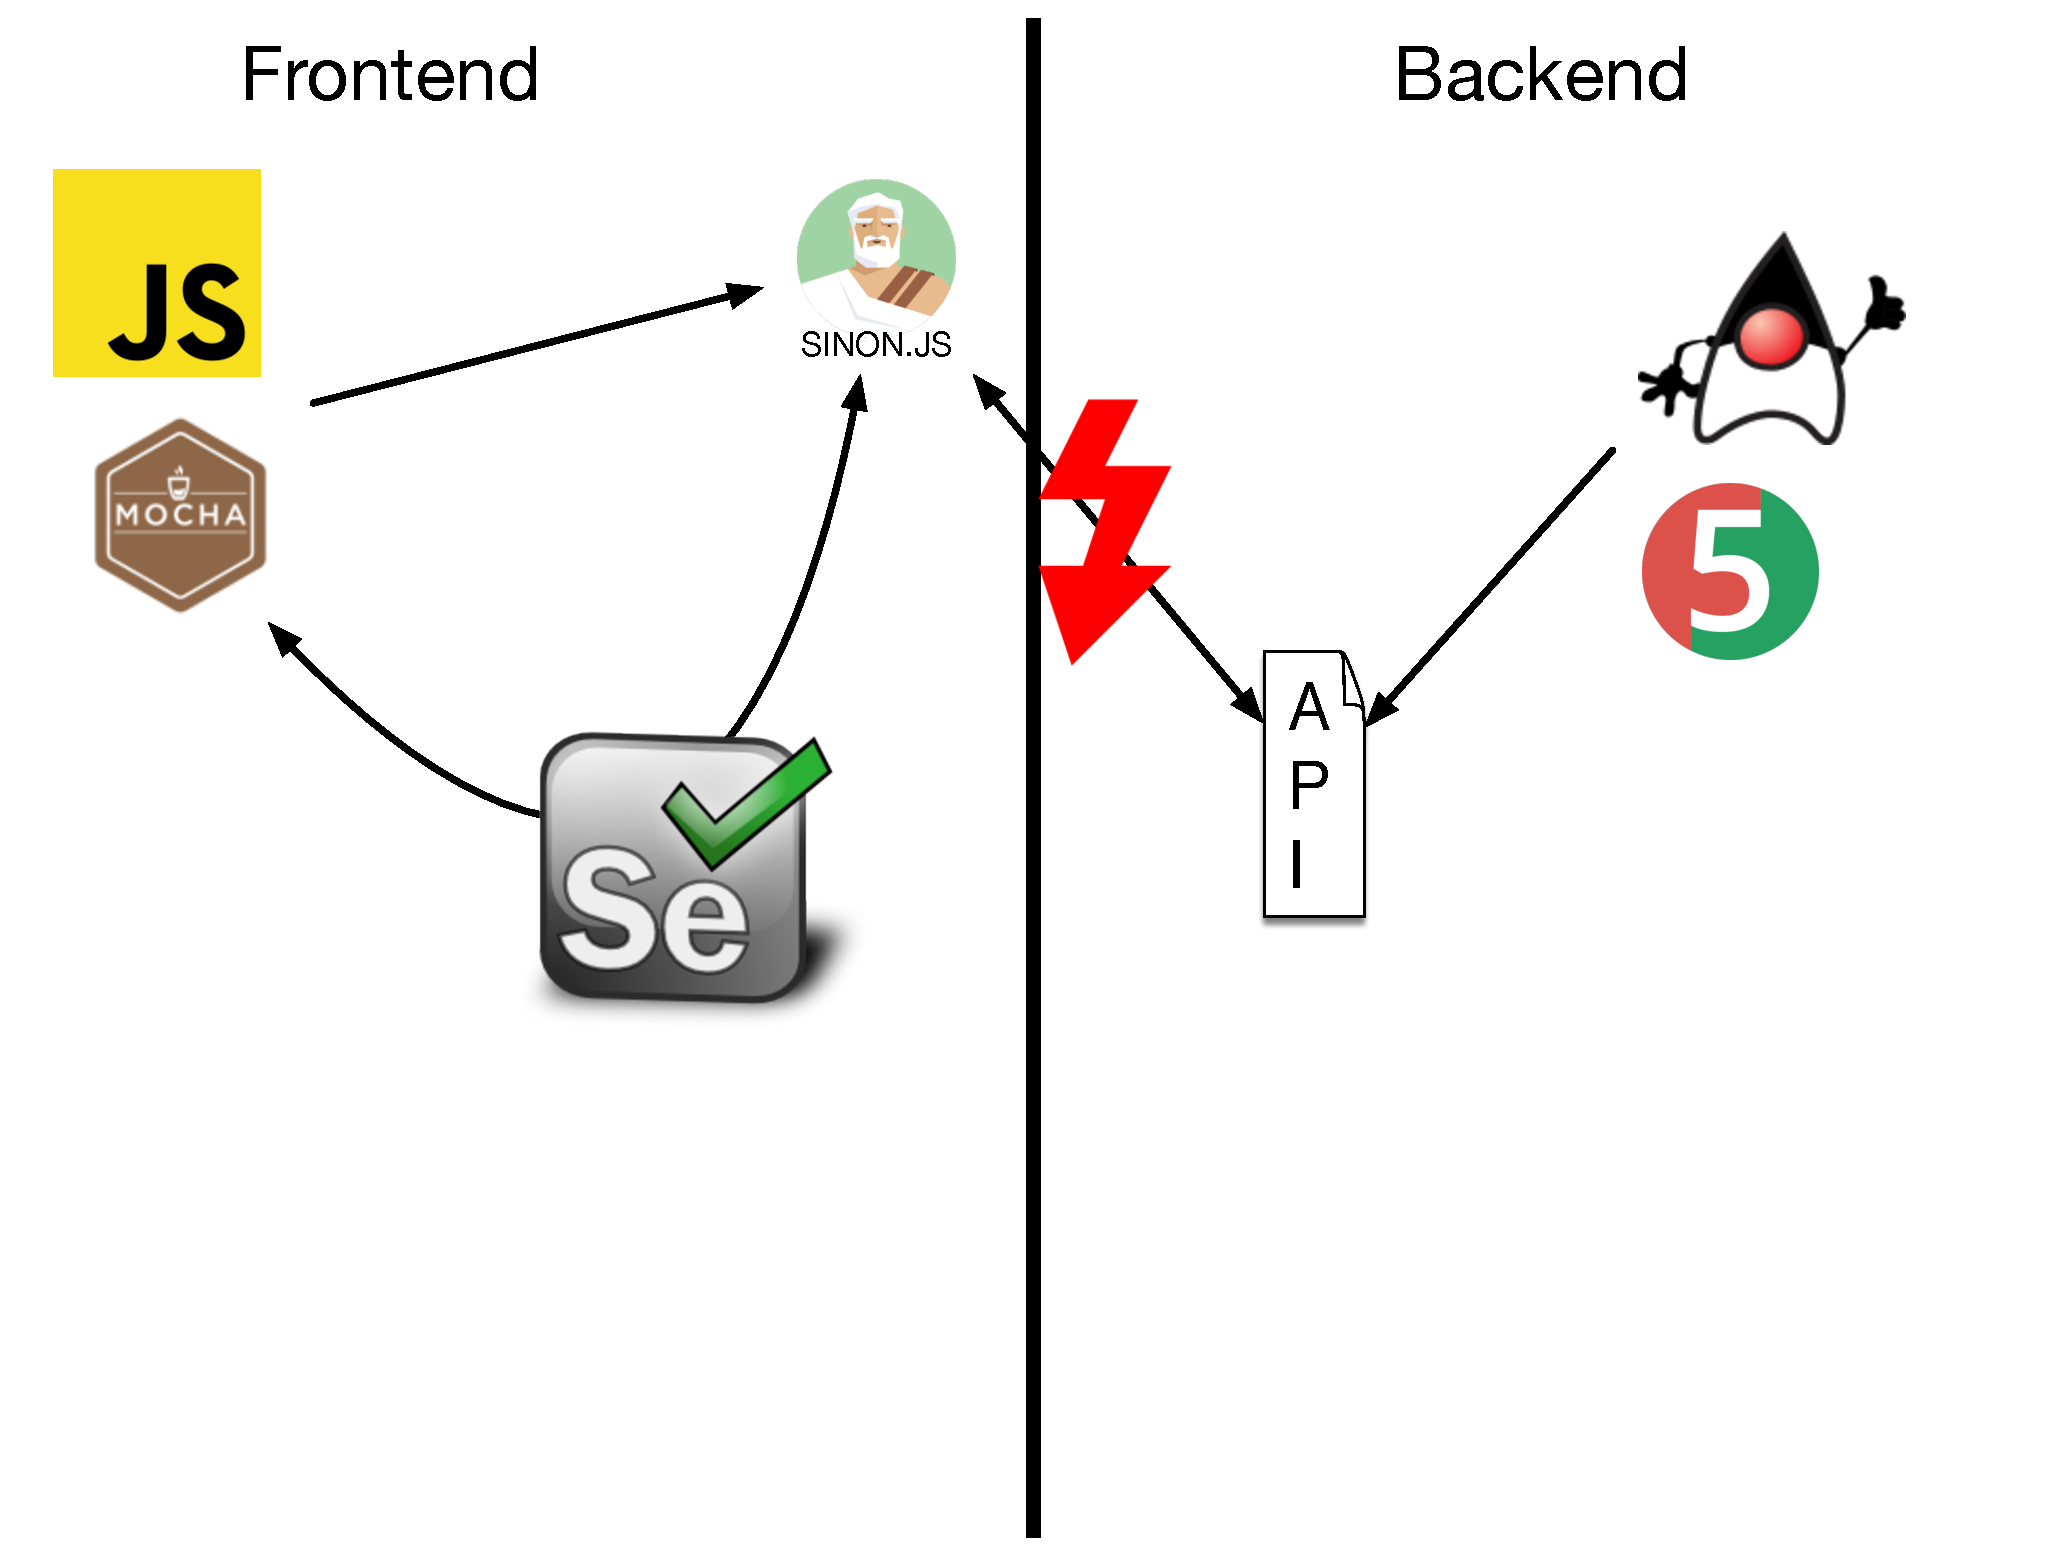
\includegraphics[width=\textwidth]{images/still-quite-naive-approach-7.pdf}
}

\end{frame}

%%%%%%%%%%%%%%%%%%%%%%%%%%%%%%%%%%%%%%%%%%%%%%%%%%
\begin{frame}[fragile]{}

\begin{center}
{\Huge
``Industry-Strength'' Approach: \\[1em]
Consumer-Driven Contract Testing
}
\end{center}

\end{frame}

\begin{frame}[fragile]{}

\only<1>{
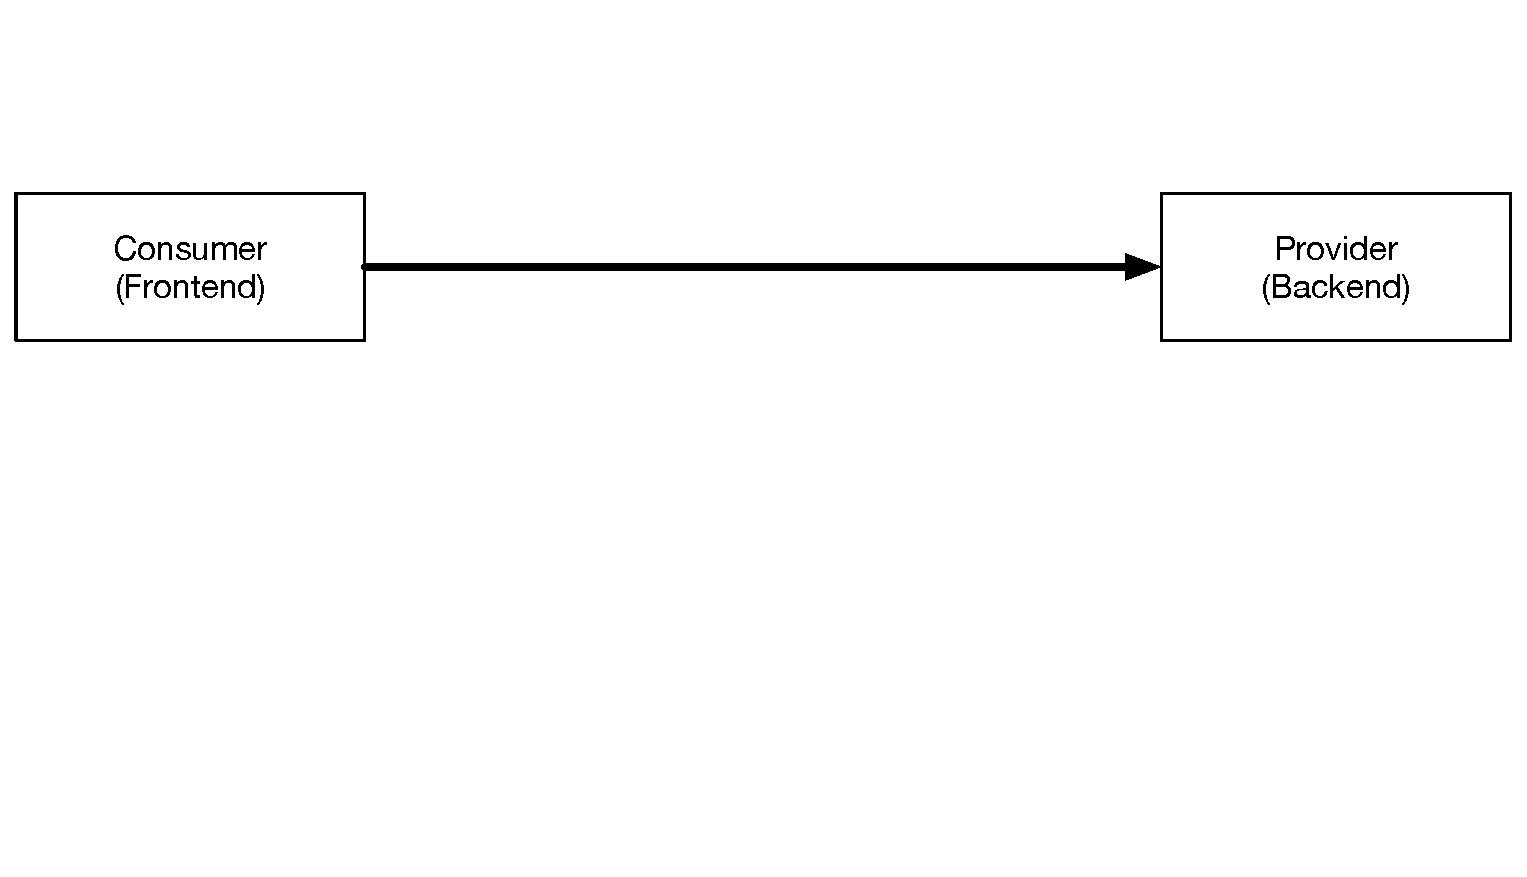
\includegraphics[width=\textwidth]{images/CDCT1.pdf}
}

\only<2>{
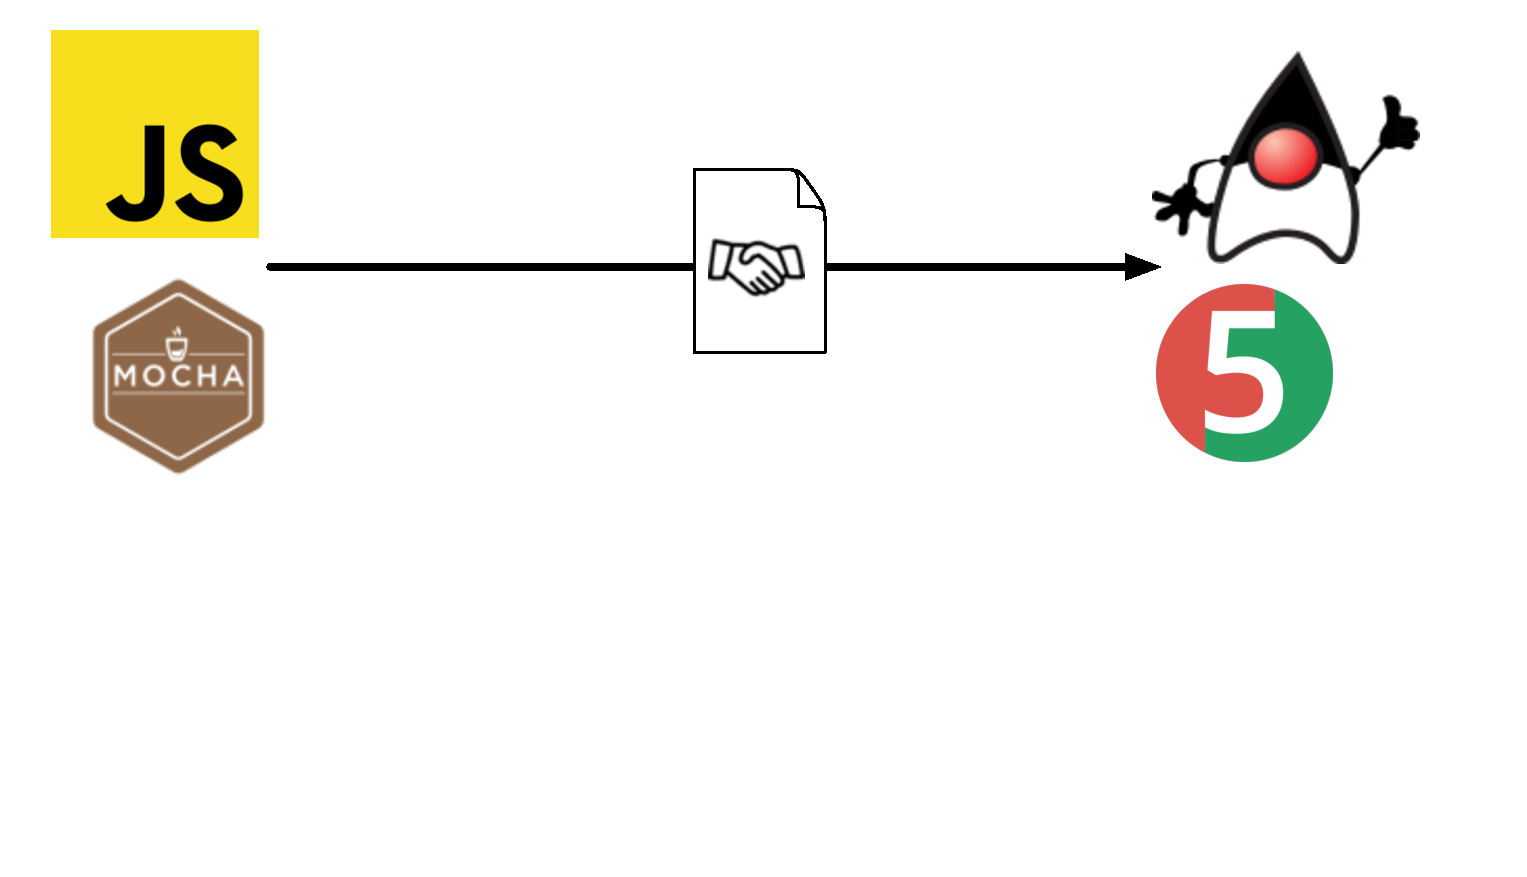
\includegraphics[width=\textwidth]{images/CDCT2.pdf}
}

\only<3>{
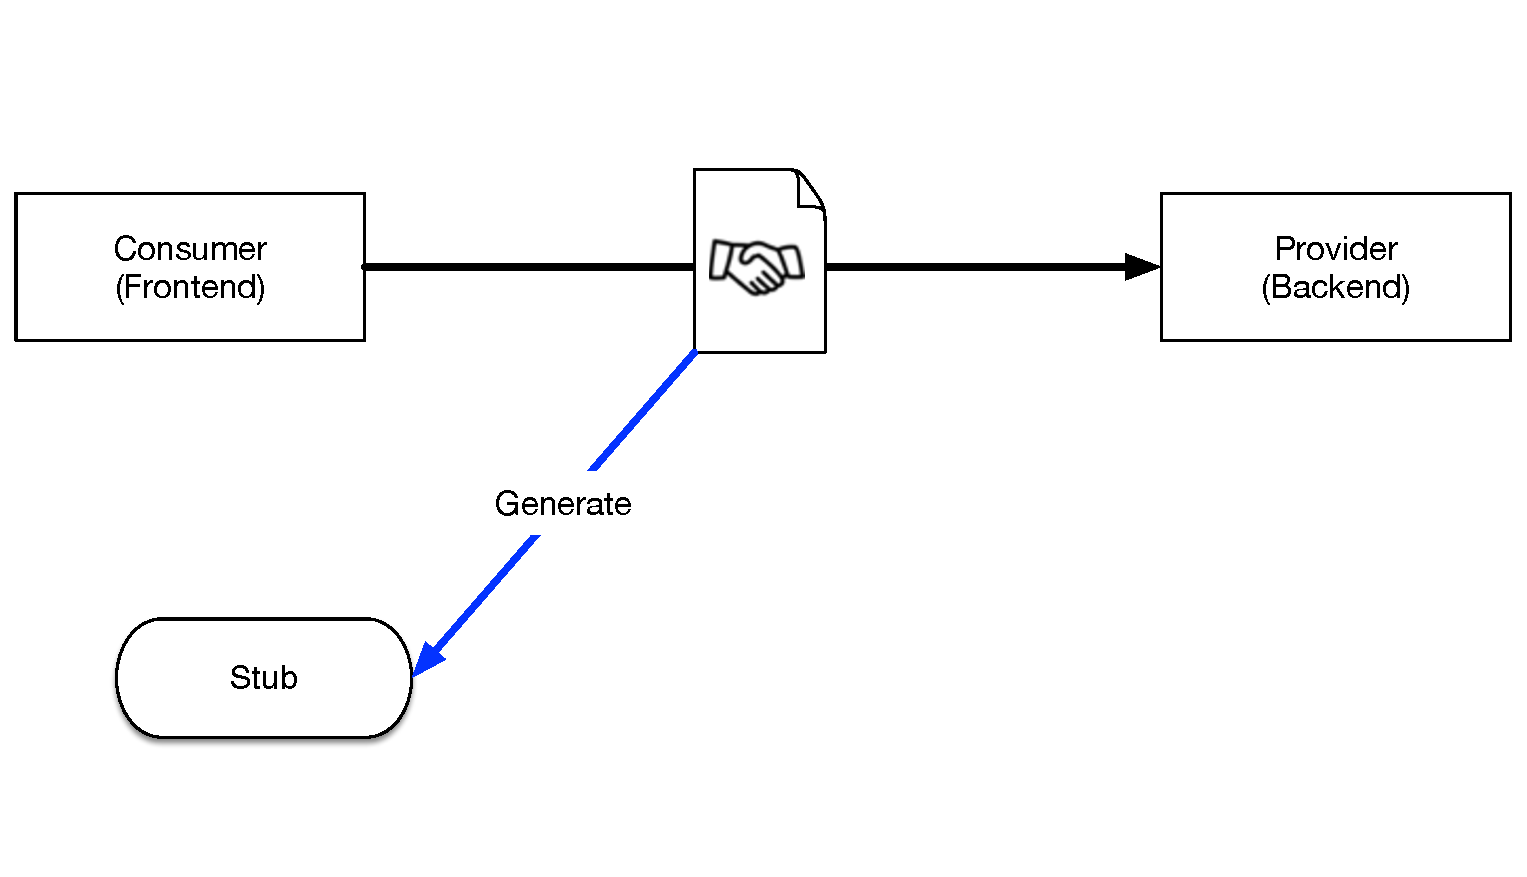
\includegraphics[width=\textwidth]{images/CDCT3.pdf}
}

\only<4>{
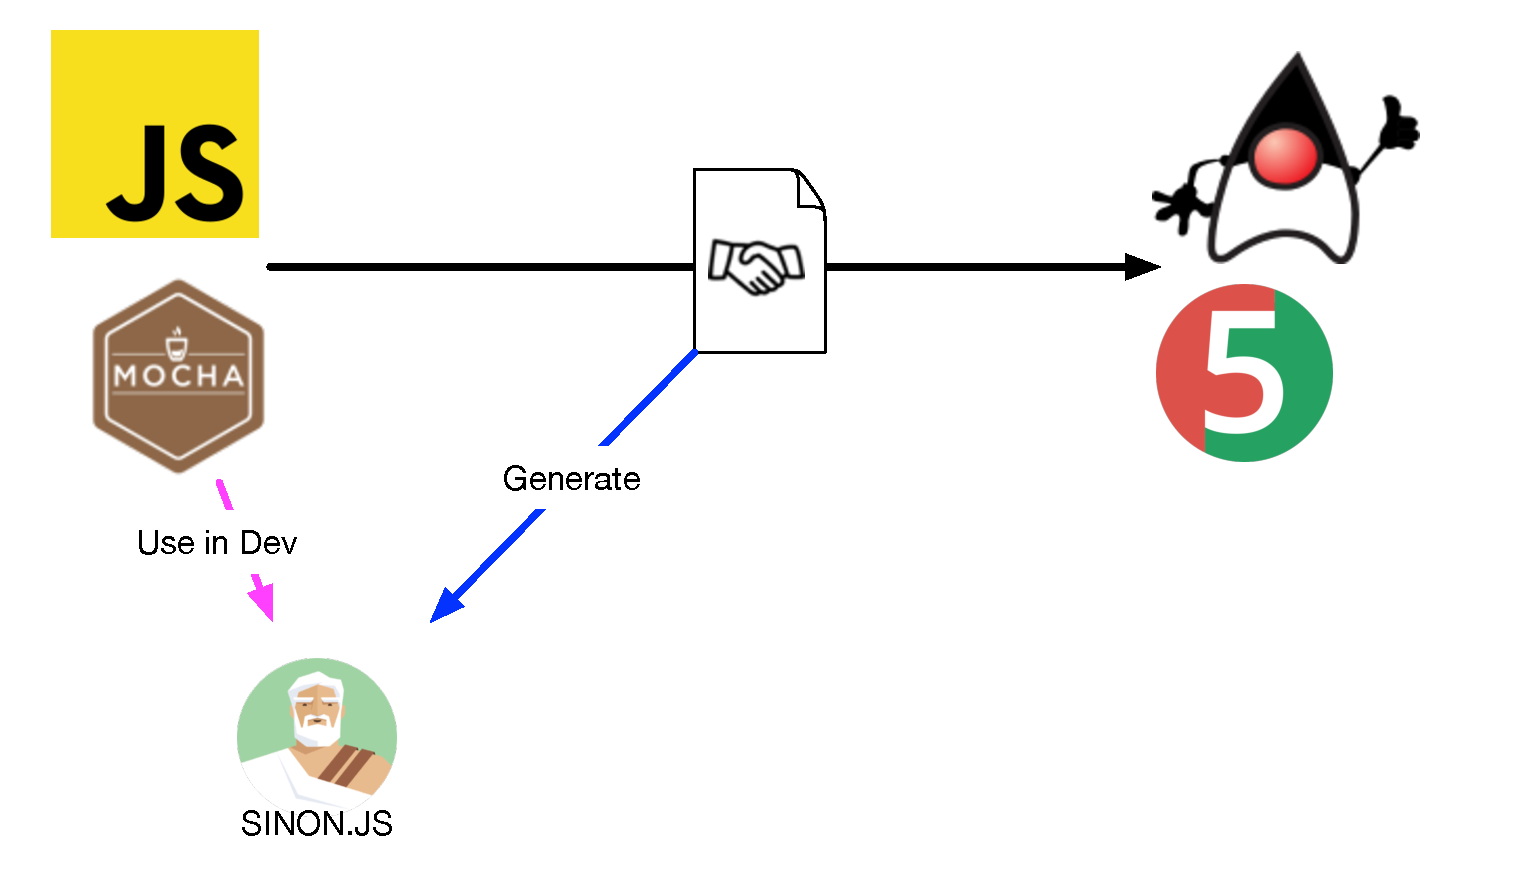
\includegraphics[width=\textwidth]{images/CDCT4.pdf}
}

\only<5>{
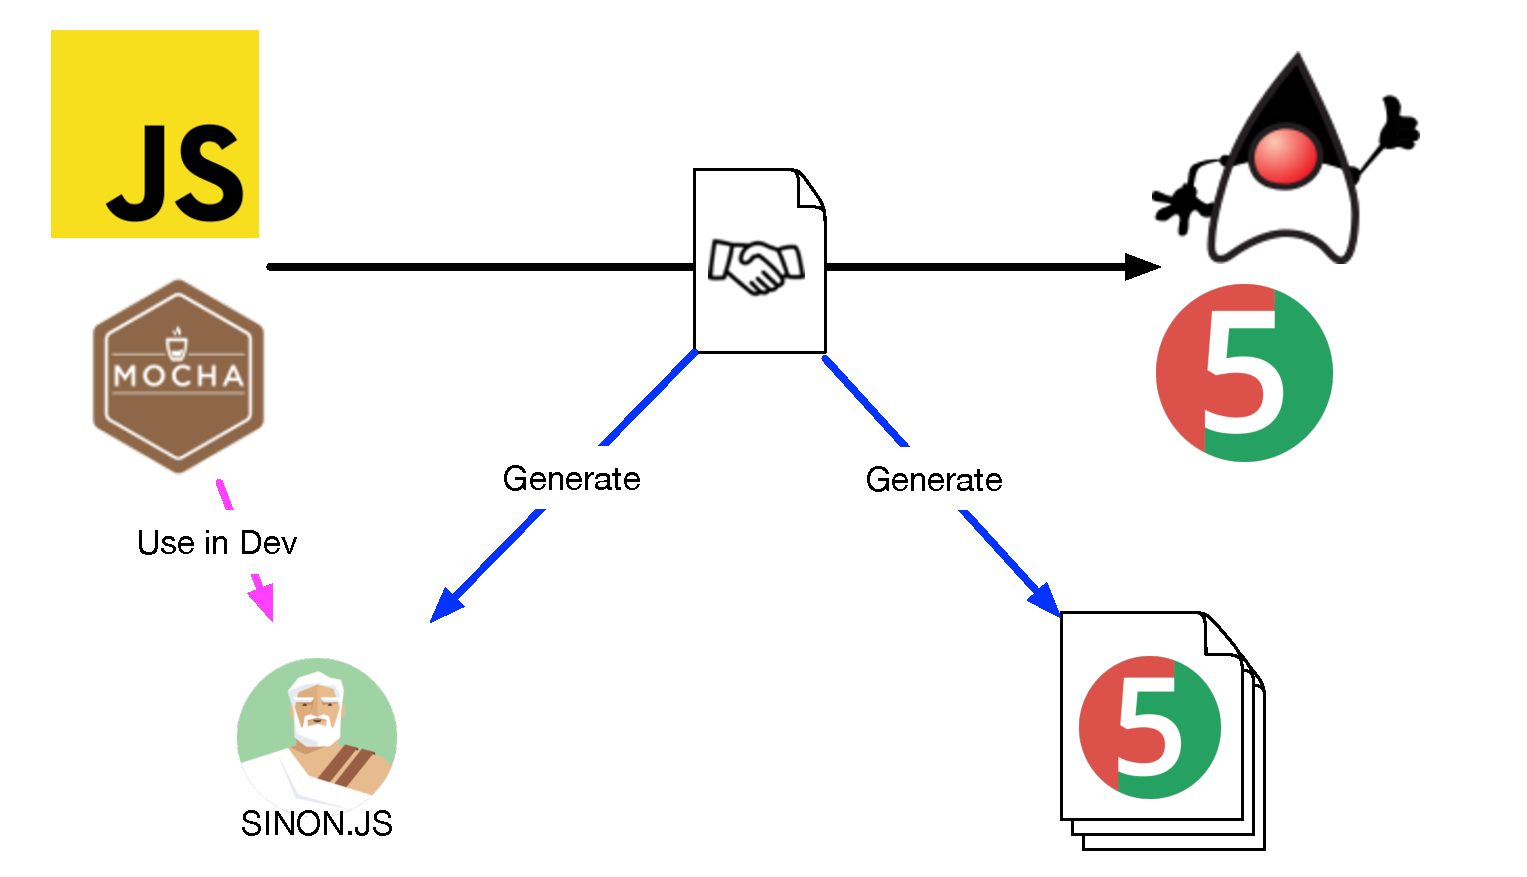
\includegraphics[width=\textwidth]{images/CDCT5.pdf}
}

\only<6>{
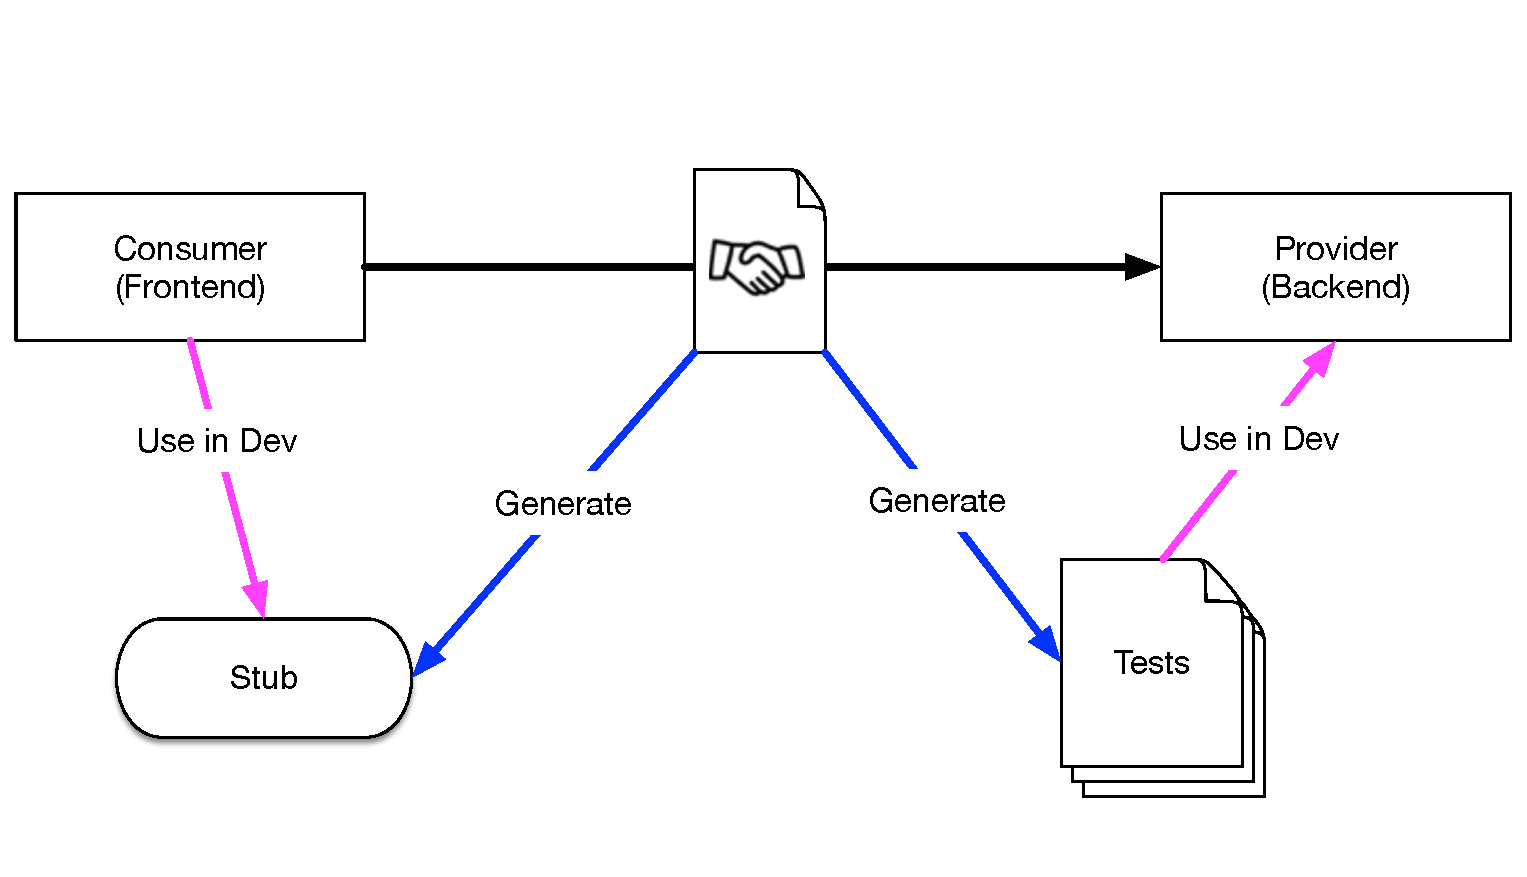
\includegraphics[width=\textwidth]{images/CDCT6.pdf}
}

\only<7>{
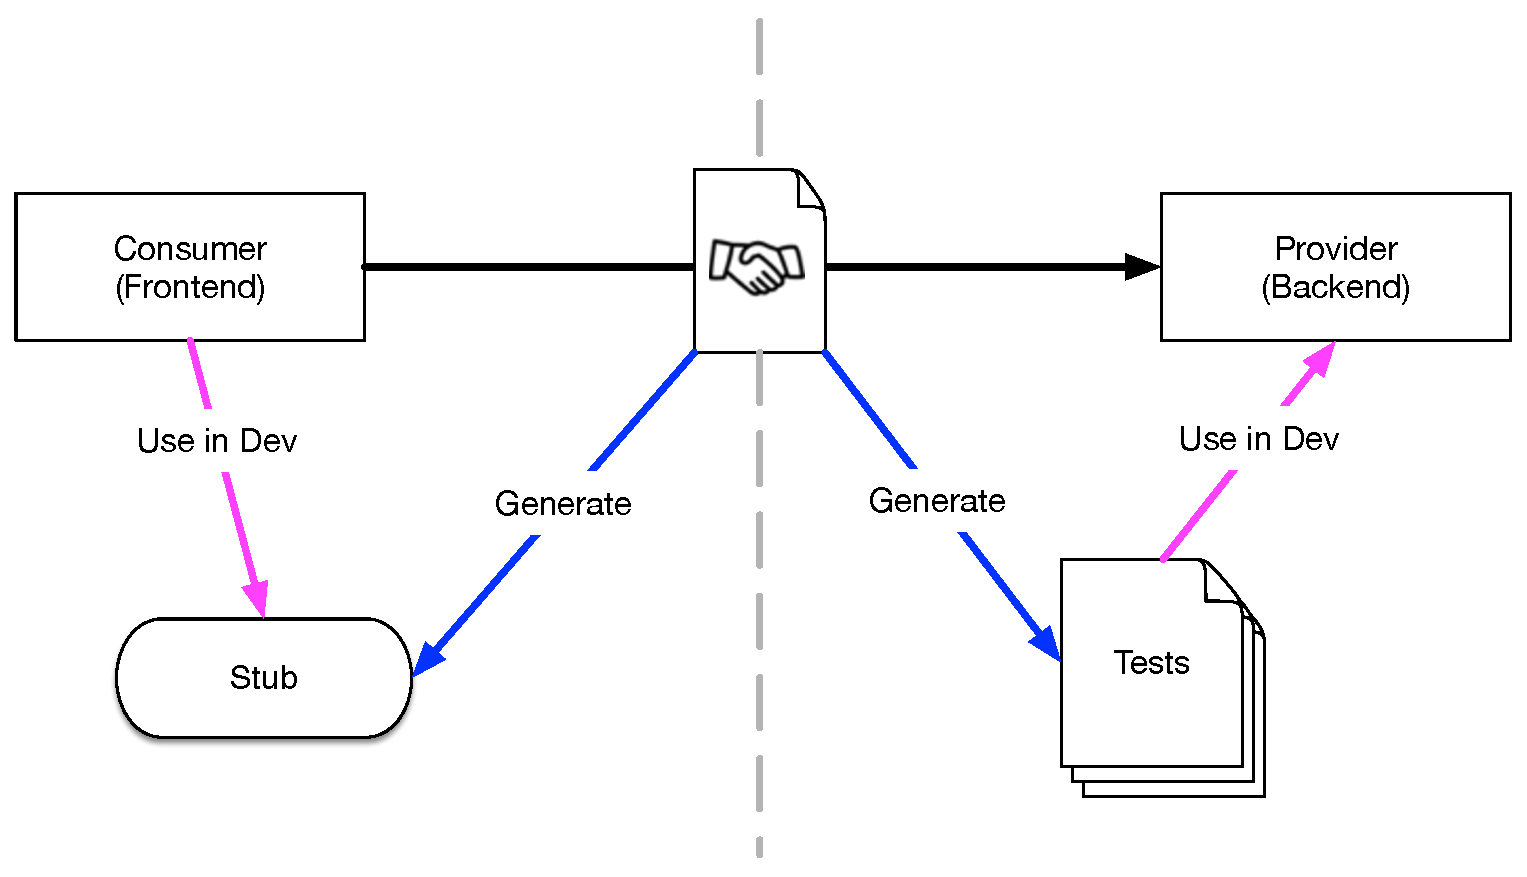
\includegraphics[width=\textwidth]{images/CDCT7.pdf}
}

\end{frame}

%%%%%%%%%%%%%%%%%%%%%%%%%%%%%%%%%%%%%%%%%%%%%%%%%%
\begin{frame}[fragile]{Example: Pet Store Domain}

\begin{itemize}
\item List all pets
\item Add pet
\item Remove pet
\end{itemize}

\end{frame}

%%%%%%%%%%%%%%%%%%%%%%%%%%%%%%%%%%%%%%%%%%%%%%%%%%
\begin{frame}[fragile]{Example: Pet Store Contracts I}

  \lstinputlisting{contracts/nopets}

\end{frame}


\begin{frame}[fragile]{Situation}

\begin{itemize}[<+->]
\item GET-Request
\item Does not depend on state
\item Easy to handle with CDCT
\end{itemize}
\end{frame}

\begin{frame}[fragile]{Questions}

\begin{itemize}[<+->]
\item Completeness
\begin{itemize}
\item Did we really document all requests (+ responses) in our contract?
\end{itemize}
\end{itemize}

\end{frame}


%%%%%%%%%%%%%%%%%%%%%%%%%%%%%%%%%%%%%%%%%%%%%%%%%%
\begin{frame}[fragile]{Example: Pet Store Contracts II}

  \lstinputlisting{contracts/somepets}

\end{frame}


\begin{frame}[fragile]{Situation}

\begin{itemize}[<+->]
\item GET-Request that depends on state
\item POST-/PUT-/DELETE-Requests
\item Difficult to handle with CDCT
\item Backend state needs to be established somehow
\item State checks need to be established somehow
\end{itemize}
\end{frame}


\begin{frame}[fragile]{Questions}

\begin{itemize}[<+->]
\item Completeness
\begin{itemize}
\item Did we really document all requests (+ responses) in our contract?
\item All possible combinations with different backend states?
\end{itemize}

\vspace{1em}
\item State Validity
\begin{itemize}
\item What are valid states in our stub?
\item Did we always establish a valid state in our stub?
\item How do we establish them (technically) before the request?
\item How do we validate them after the (modifying) request?
\end{itemize}

\vspace{1em}
\item Maintenance
\begin{itemize}
\item How can we keep track of our contracts and avoid redundancies?
\item How can we effectively maintain the contracts in case of changes?
\end{itemize}
\end{itemize}

\end{frame}

%%%%%%%%%%%%%%%%%%%%%%%%%%%%%%%%%%%%%%%%%%%%%%%%%%
\begin{frame}[fragile]{}

\begin{center}
{\Huge
We need the Functional Essence!
}
\end{center}

\end{frame}

\begin{frame}[fragile]{}
\vspace{-.65em}
\begin{center}
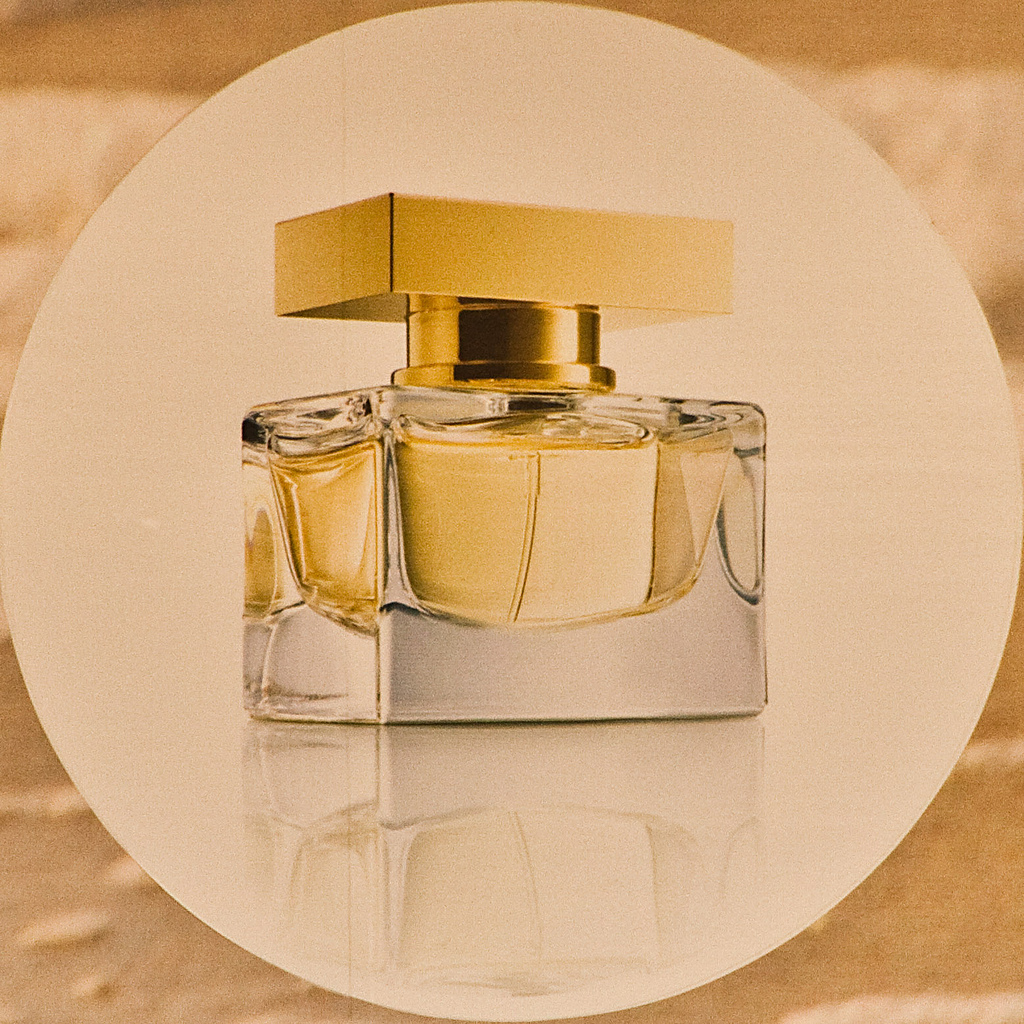
\includegraphics[height=\paperheight]{images/essence_large}
\end{center}

\end{frame}

%%%%%%%%%%%%%%%%%%%%%%%%%%%%%%%%%%%%%%%%%%%%%%%%%%
\begin{frame}[fragile]{}

\begin{center}
{\Huge
Sounds cool, but$\ldots$

\onslide<2->
\vspace{1.5em}
$\ldots$what does that mean?
}
\end{center}

\end{frame}

%%%%%%%%%%%%%%%%%%%%%%%%%%%%%%%%%%%%%%%%%%%%%%%%%%
\begin{frame}[fragile]{Functional Essence}

\begin{itemize}[<+->]
\item Fake Server
\item Lightweight Implementation

\vspace{1em}

\item Model

\vspace{1em}

\item Rapid Prototype
\item Minimal Viable Product
\end{itemize}

\end{frame}

%%%%%%%%%%%%%%%%%%%%%%%%%%%%%%%%%%%%%%%%%%%%%%%%%%
\begin{frame}[fragile]{Functional Essence Serves Many Purposes}

\begin{itemize}[<+->]
\item To learn about the domain
\item To discuss with domain experts
\item To validate assumptions at an early stage

\vspace{1em}

\item To check the real implementation:
\end{itemize}

\end{frame}

%%%%%%%%%%%%%%%%%%%%%%%%%%%%%%%%%%%%%%%%%%%%%%%%%%

% TODO Essence in Bilder einfügen

\begin{frame}[fragile]{}

\only<1>{
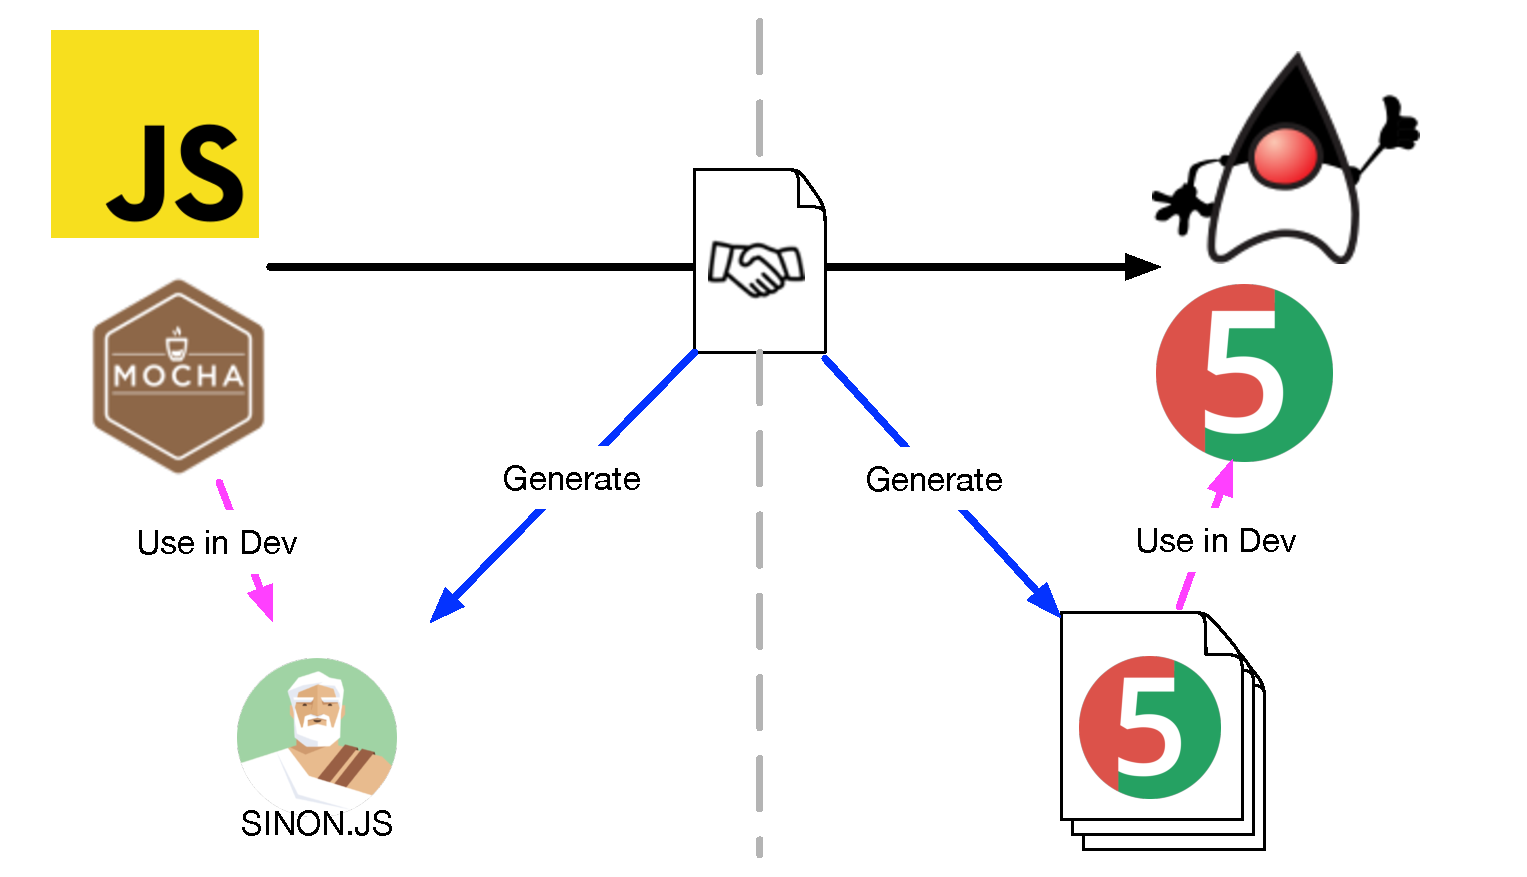
\includegraphics[width=\textwidth]{images/Essence-1.pdf}
}

\only<2>{
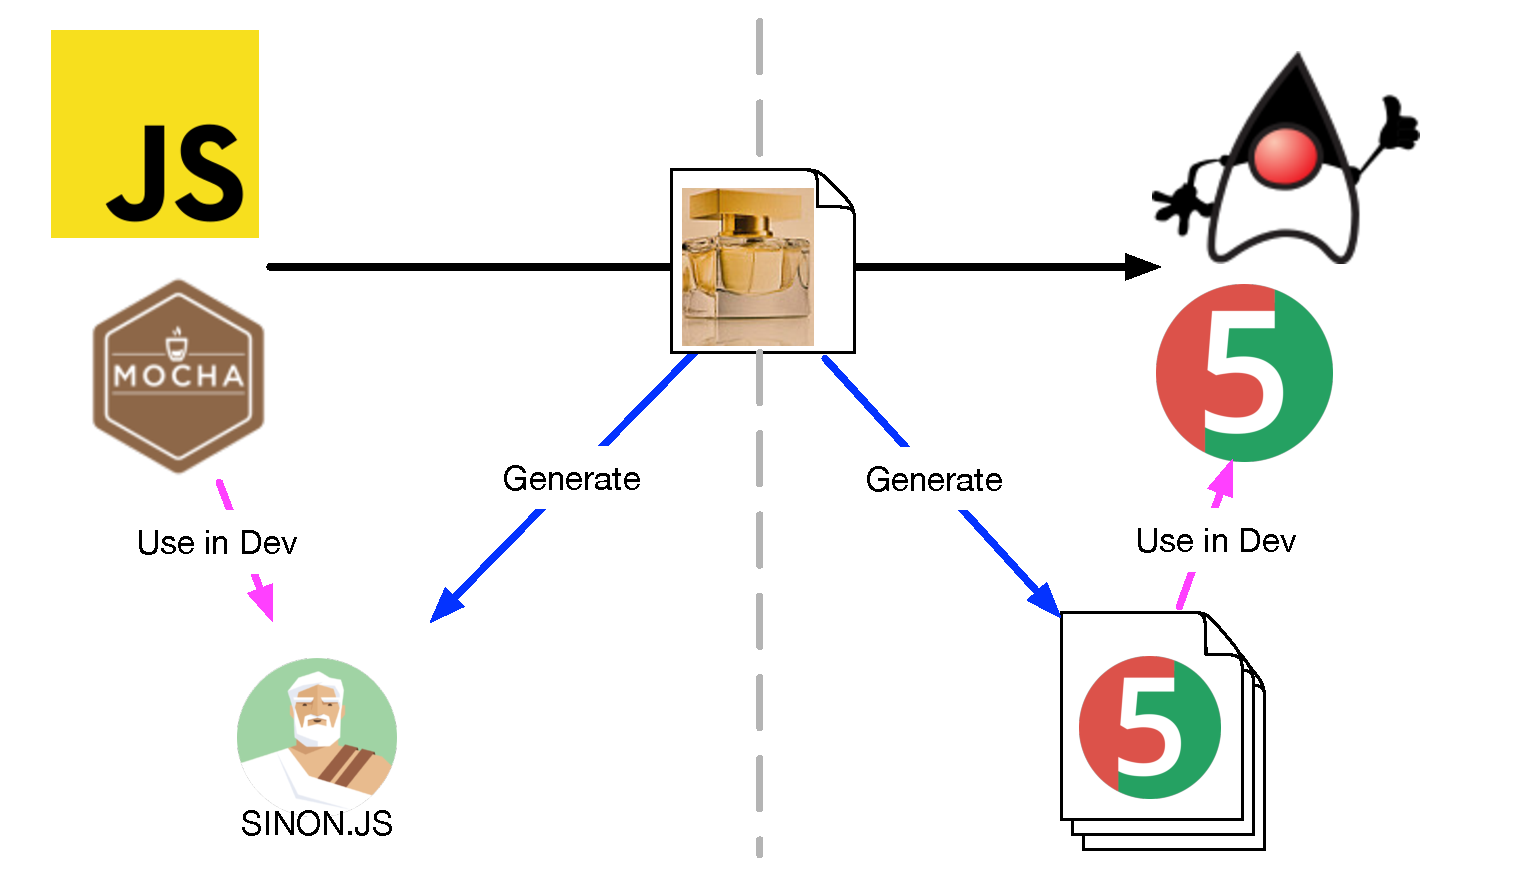
\includegraphics[width=\textwidth]{images/Essence-2.pdf}
}

\only<3>{
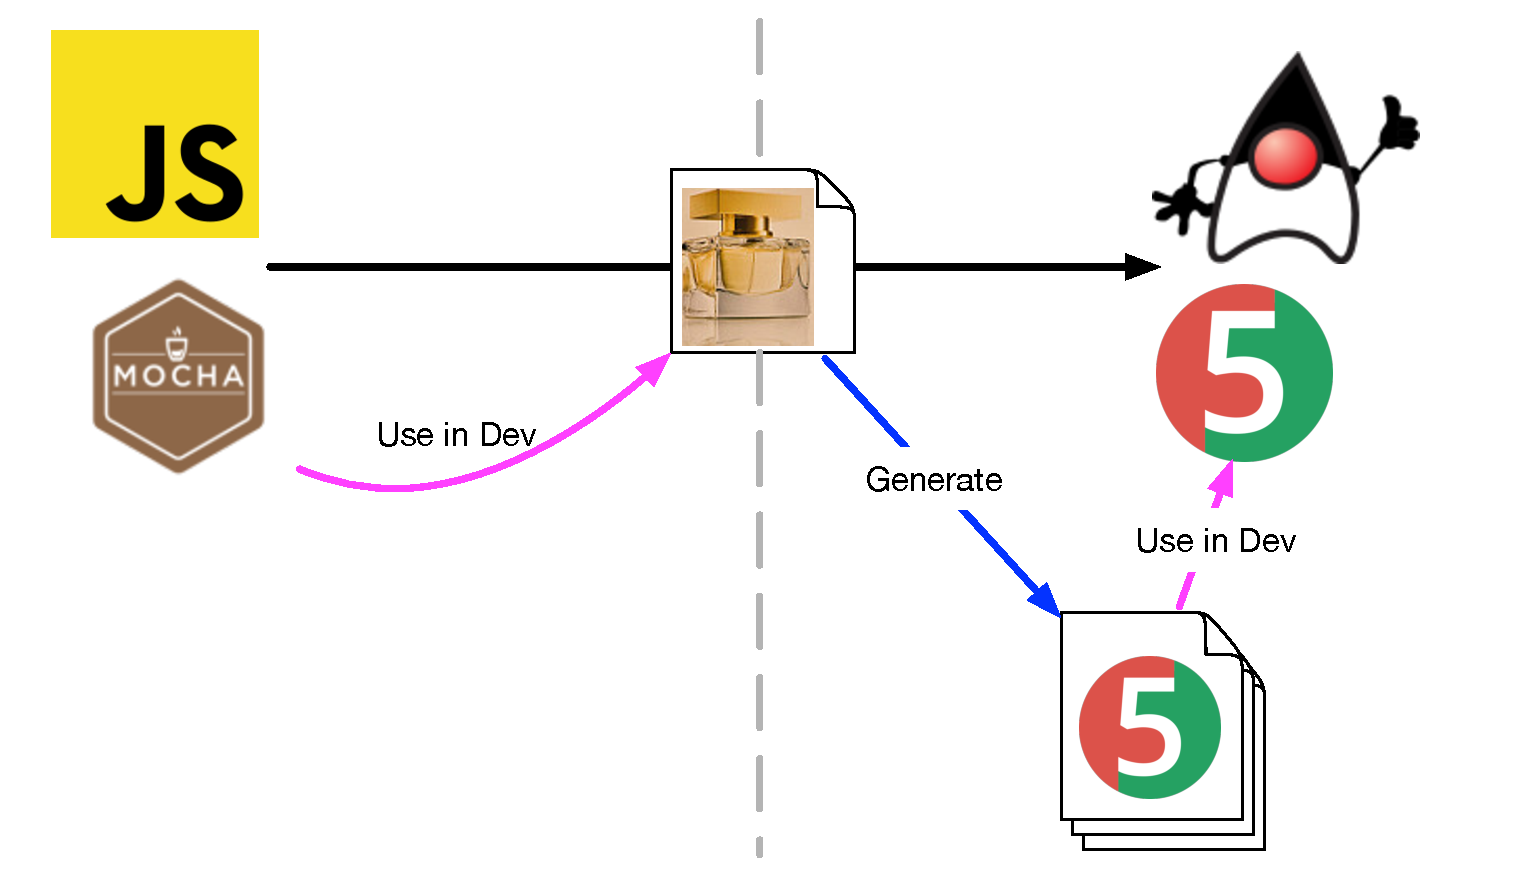
\includegraphics[width=\textwidth]{images/Essence-3.pdf}
}

\only<4>{
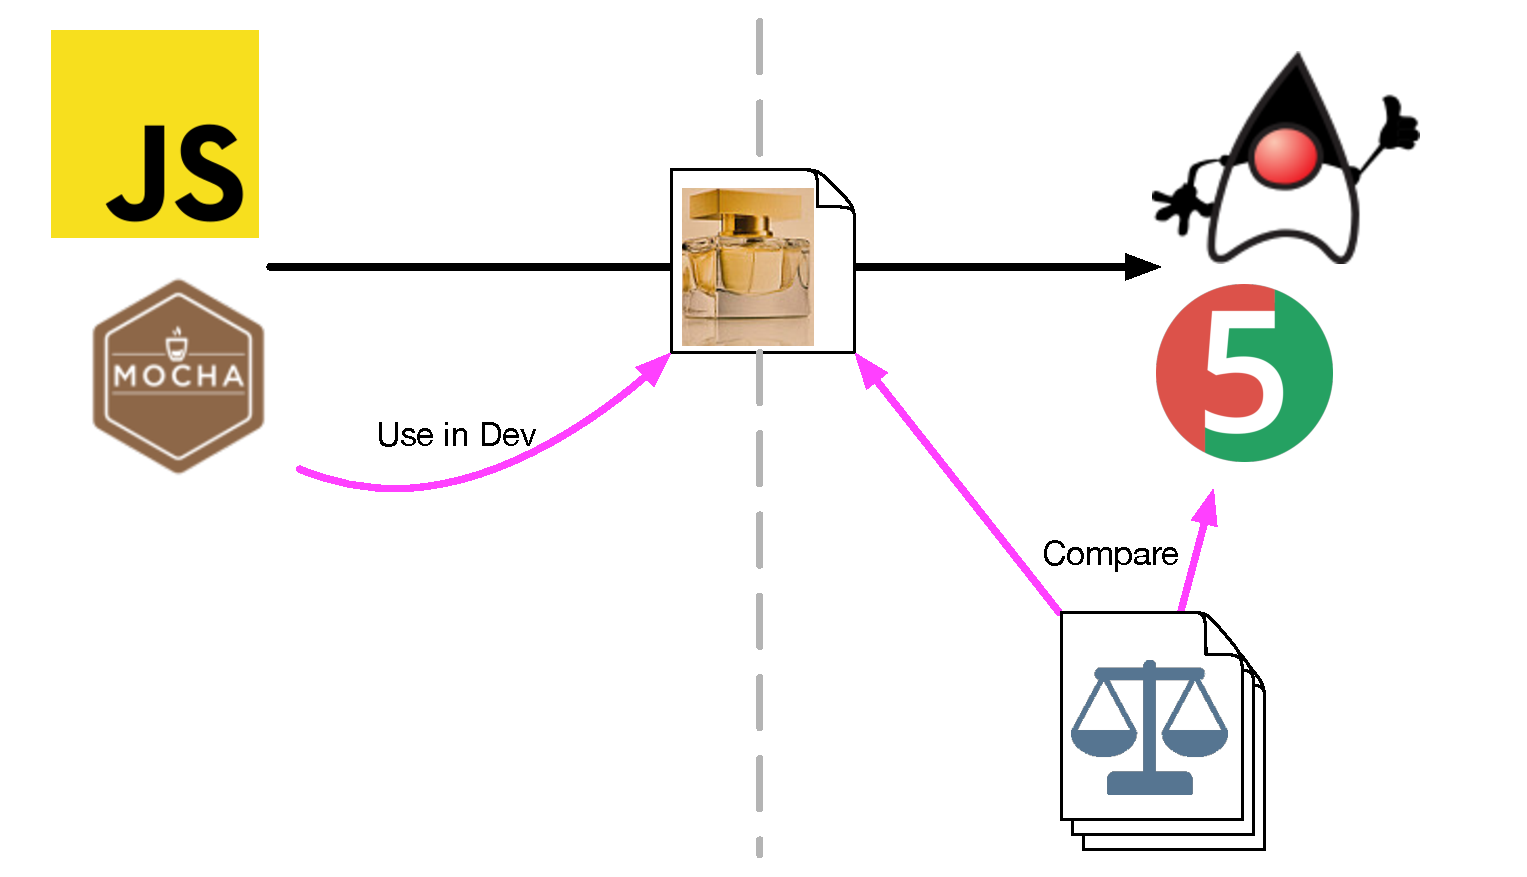
\includegraphics[width=\textwidth]{images/Essence-4.pdf}
}

\end{frame}


%%%%%%%%%%%%%%%%%%%%%%%%%%%%%%%%%%%%%%%%%%%%%%%%%%
\begin{frame}[fragile]{}

\begin{center}
{\Huge
Sounds cool, but$\ldots$

\onslide<2->
\vspace{1.5em}
$\ldots$how can I build this?
}
\end{center}

\end{frame}

%%%%%%%%%%%%%%%%%%%%%%%%%%%%%%%%%%%%%%%%%%%%%%%%%%
\begin{frame}[fragile]{How to Build a Functional Essence}

\begin{itemize}[<+->]
\item Implement the domain logic
\item In the simplest possible way
\item In an arbitrary language
\end{itemize}

\vspace{2em}

\onslide<+->
\begin{center}
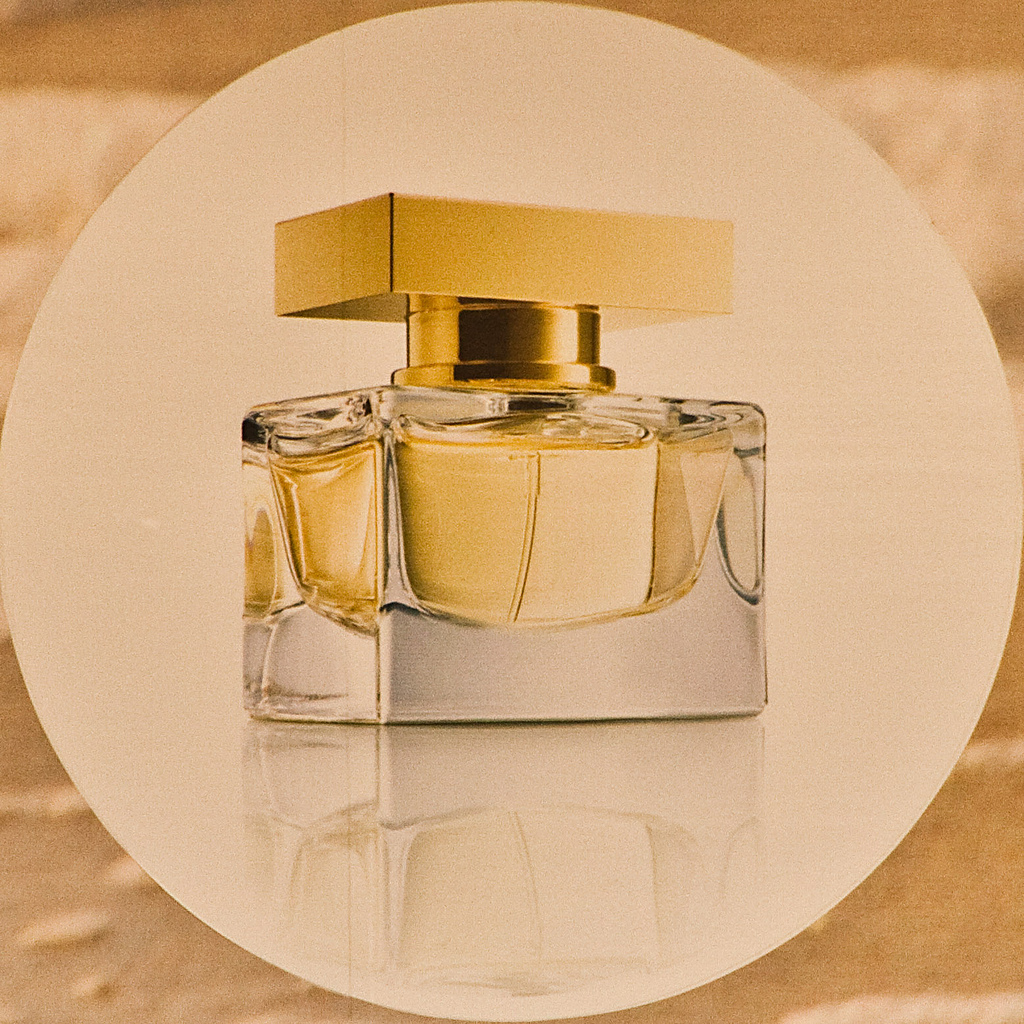
\includegraphics[width=.3\textwidth]{images/essence_large.jpg}
\end{center}

\end{frame}

\begin{frame}[fragile]{The Pets Essence}

\begin{lstlisting}[language=JavaScript]
class Pets {
    constructor(){
        this._pets = [];
    }

    getPets() {
        return petSorter.sortPets(this._pets);
    }

    addPet(pet) {
        this._pets.push(pet);
        return 'Pet successfully added.';
    }

    removePet(pet) {
        this._pets = this._pets.filter(
            p => p.petName !== pet.petName || p.petType !== pet.petType);
        return 'Pet successfully removed.';
    }
}
\end{lstlisting}

\end{frame}

\begin{frame}[fragile]{The Overall Essence}

\begin{lstlisting}[language=Javascript]
class Essence {
    constructor() {
        this._pets = new Pets();
        this._somethingElse = new SomethingElse();
    }

    pets() {
        return this._pets;
    }
    
    somethingElse() {
        return this._somethingElse;
    }
}
\end{lstlisting}

\end{frame}

\begin{frame}[fragile]{The Essence App}

\begin{lstlisting}[language=Javascript]
let essence = new Essence();

router.get('/pets', (req, res) => {
    const pets = essence.pets().getPets();
    res.json({tag: 'Pets', pets});
});

router.post('/pets', (req, res) => {
    const message = essence.pets().addPet({ petName: req.body.petName, petPrice: req.body.petPrice, petType: req.body.petType });
    res.json({message});
});

router.delete('/pets', (req, res) => {
    const message = essence.pets().removePet({ petName: req.body.petName, petPrice: req.body.petPrice, petType: req.body.petType });
    res.json({message});
});
\end{lstlisting}

\end{frame}


\begin{frame}[fragile]{Important Addition}

\begin{lstlisting}[language=Javascript]
router.delete('/reset', (req, res) => {
    essence = new Essence();
    res.json({message: 'All pets successfully removed.'});
});
\end{lstlisting}

\end{frame}


%%%%%%%%%%%%%%%%%%%%%%%%%%%%%%%%%%%%%%%%%%%%%%%%%%
\begin{frame}[fragile]{Isn't That The Same Code As The Backend?}

\begin{itemize}
\onslide<2->
\item Maybe$\ldots$ but usually not:
\onslide<3->
\item Can be in another language
\onslide<4->
\item Can use simpler datatypes (e.g.~List vs.~HashMap)
\onslide<5->
\item No performance-tuning (e.g.~slower but simpler algorithms)
\onslide<6->
\item No technical overhead (e.g.~database)
\onslide<7->
\item Some parts can be left out
\onslide<8->
\item $\ldots$
\end{itemize}

\end{frame}

%%%%%%%%%%%%%%%%%%%%%%%%%%%%%%%%%%%%%%%%%%%%%%%%%%
\begin{frame}[fragile]{}

\begin{center}
{\Huge
How does the Comparison work?
}
\end{center}

\end{frame}

%%%%%%%%%%%%%%%%%%%%%%%%%%%%%%%%%%%%%%%%%%%%%%%%%%
\begin{frame}[fragile]{Detour: Quick Check / Property-Based Testing}

\onslide+<2->
\begin{itemize}
\item User specifies properties
\item Tool generates examples
\item Checks properties against examples
\end{itemize}

\onslide+<3->
\begin{lstlisting}
prop_RevRev xs = reverse (reverse xs) == xs
  where types = xs::[Int]
\end{lstlisting}

\onslide+<4->
\begin{lstlisting}
Main> quickCheck prop_RevRev
OK, passed 100 tests.
\end{lstlisting}

\onslide+<5->
\begin{lstlisting}
prop_RevId xs = reverse xs == xs
  where types = xs::[Int]
\end{lstlisting}

\onslide+<6->
\begin{lstlisting}
Main> quickCheck prop_RevId
Falsifiable, after 1 tests:
[-3,15]
\end{lstlisting}

\end{frame}

%%%%%%%%%%%%%%%%%%%%%%%%%%%%%%%%%%%%%%%%%%%%%%%%%%
\begin{frame}[fragile]{}

\begin{center}
{\Huge
How to Mimic QuickCheck?
}
\end{center}

\end{frame}


\begin{frame}[fragile]{}

\begin{center}
\only<1>{
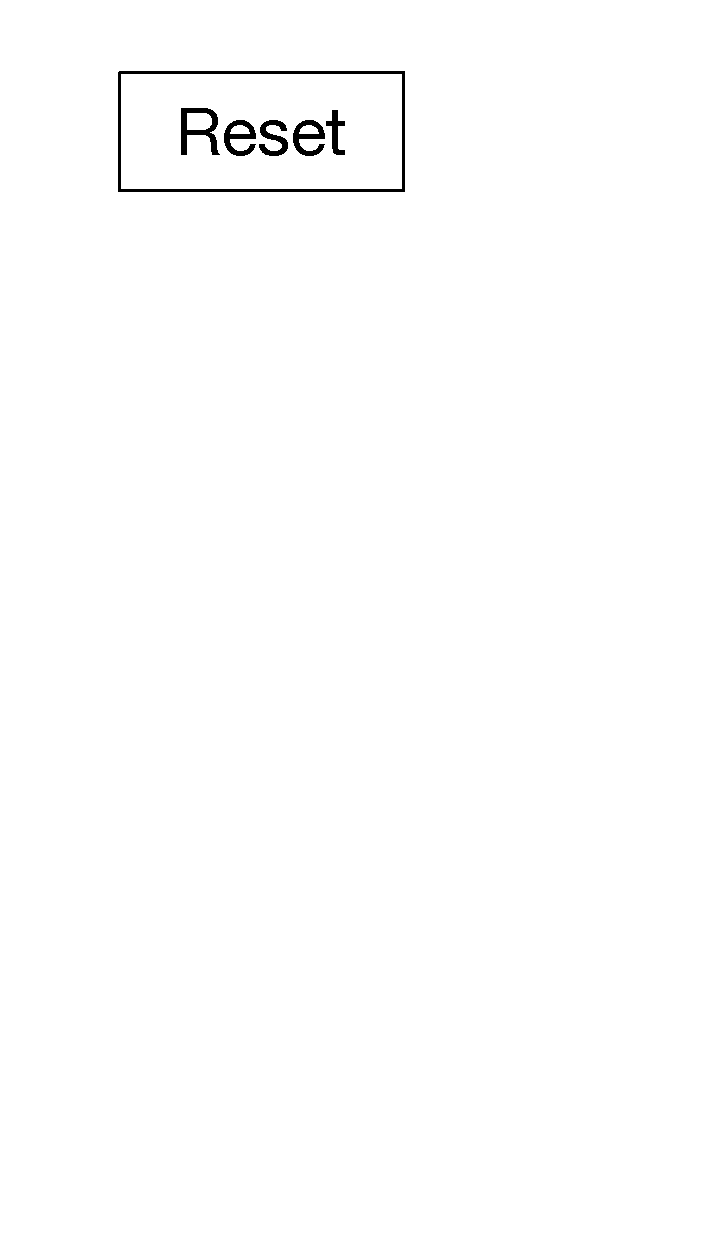
\includegraphics[height=.9\textheight]{images/Comparator-1.pdf}
}

\only<2>{
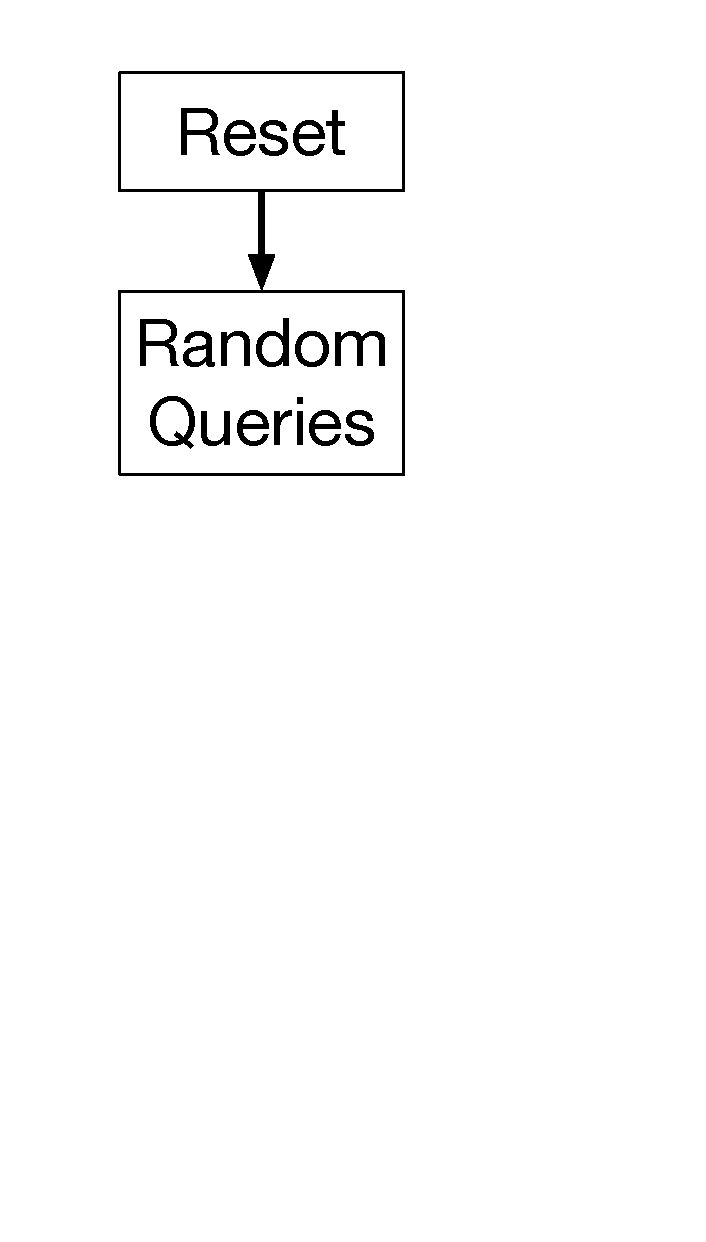
\includegraphics[height=.9\textheight]{images/Comparator-2.pdf}
}

\only<3>{
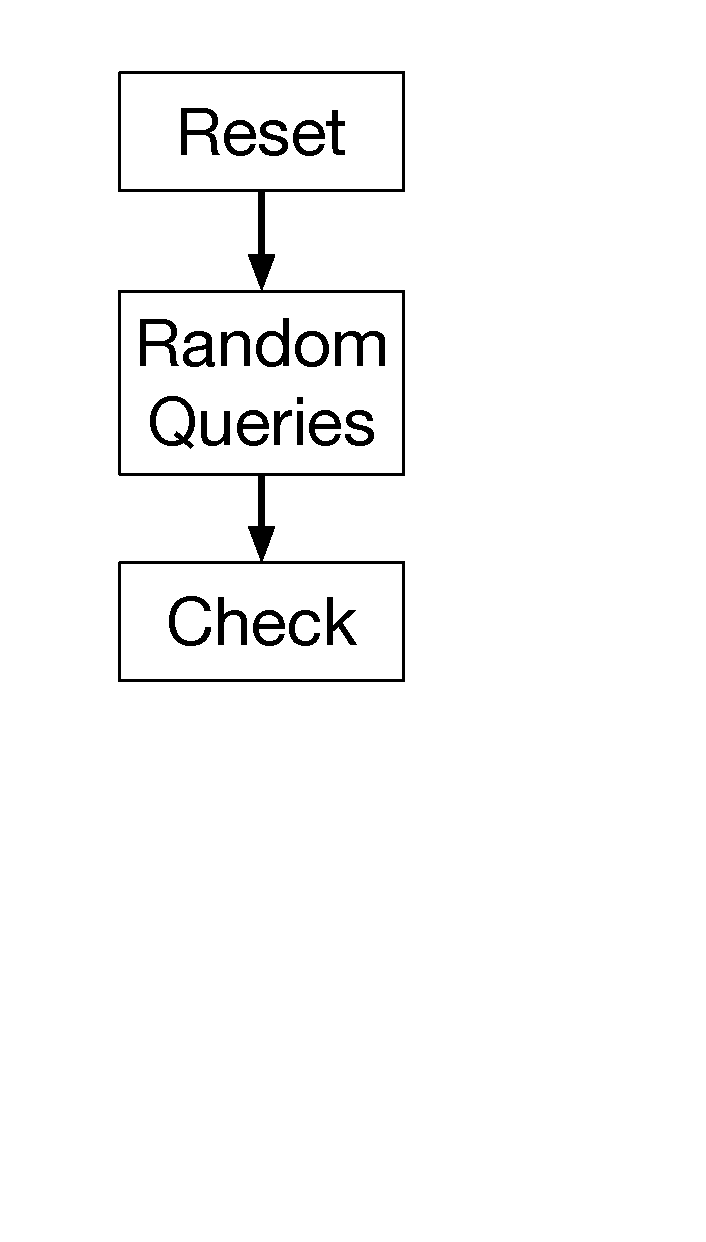
\includegraphics[height=.9\textheight]{images/Comparator-3.pdf}
}

\only<4>{
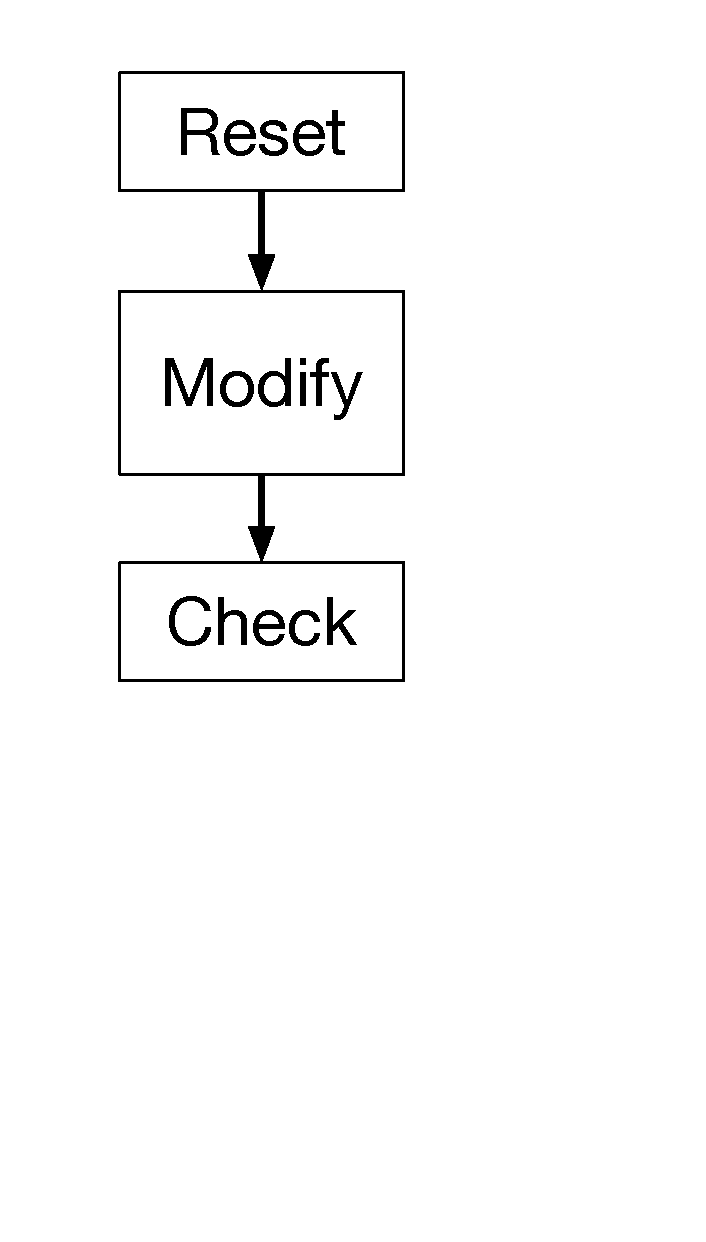
\includegraphics[height=.9\textheight]{images/Comparator-4.pdf}
}

\only<5>{
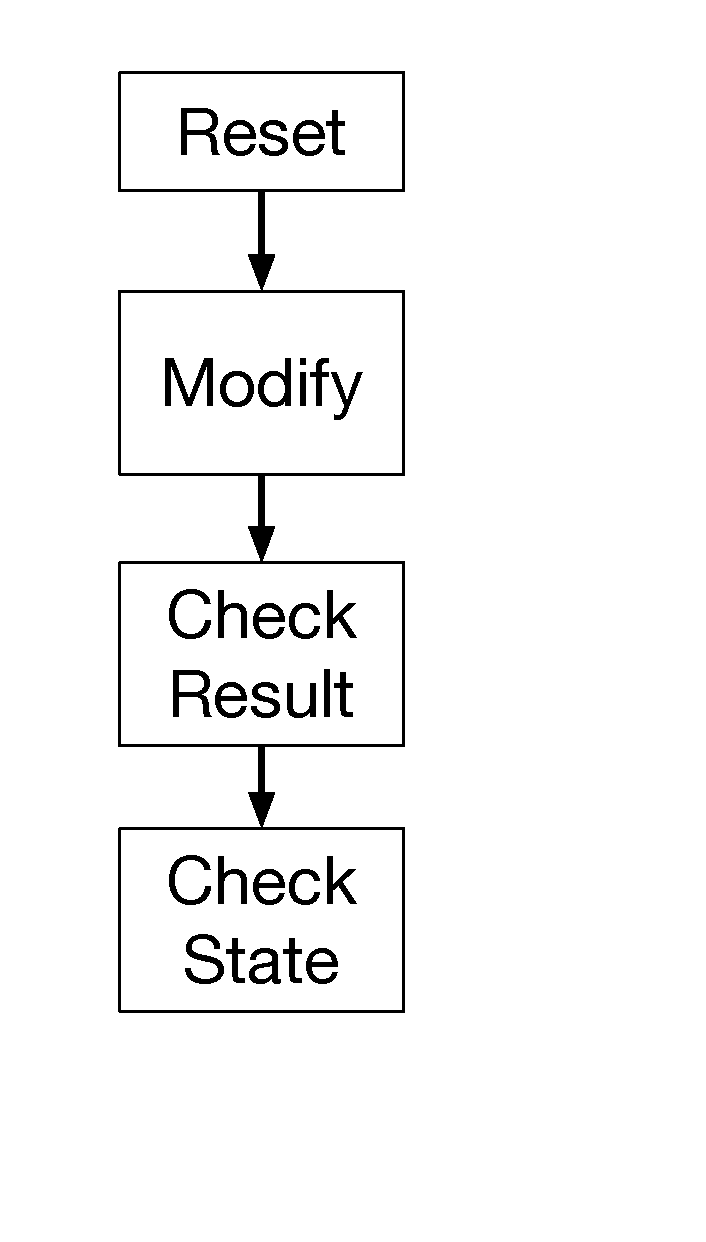
\includegraphics[height=.9\textheight]{images/Comparator-5.pdf}
}

\only<6>{
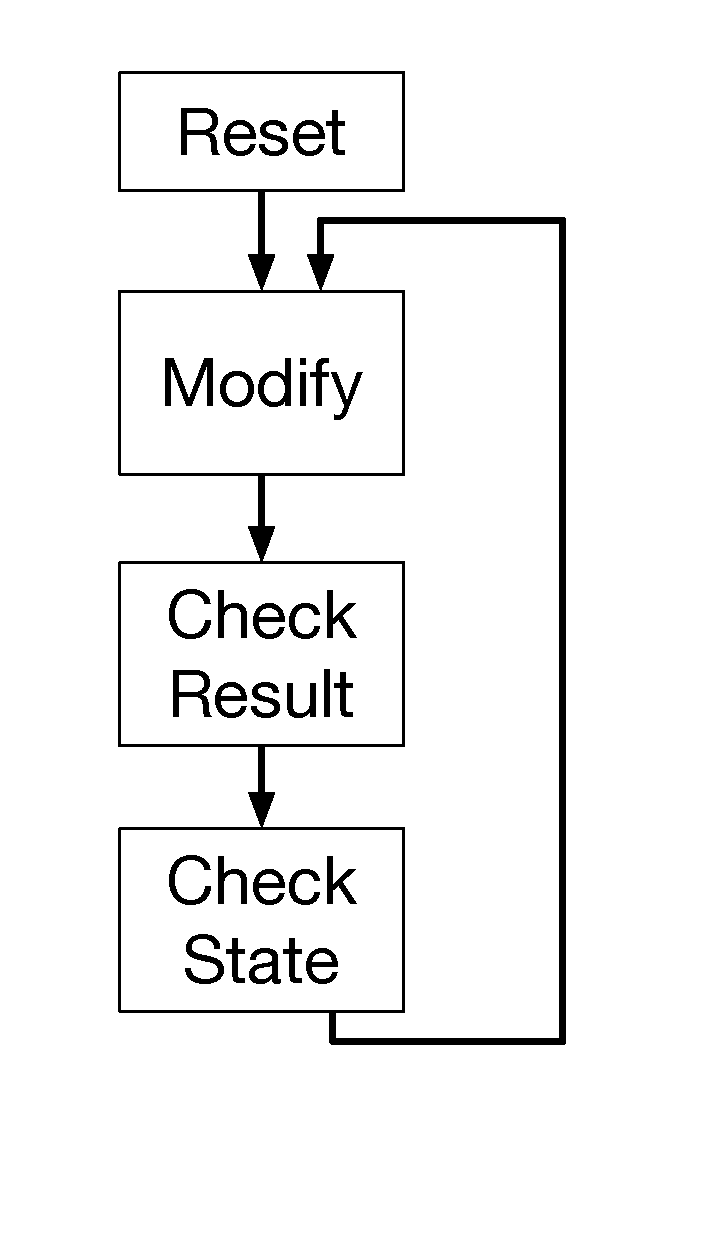
\includegraphics[height=.9\textheight]{images/Comparator-6.pdf}
}

\only<7>{
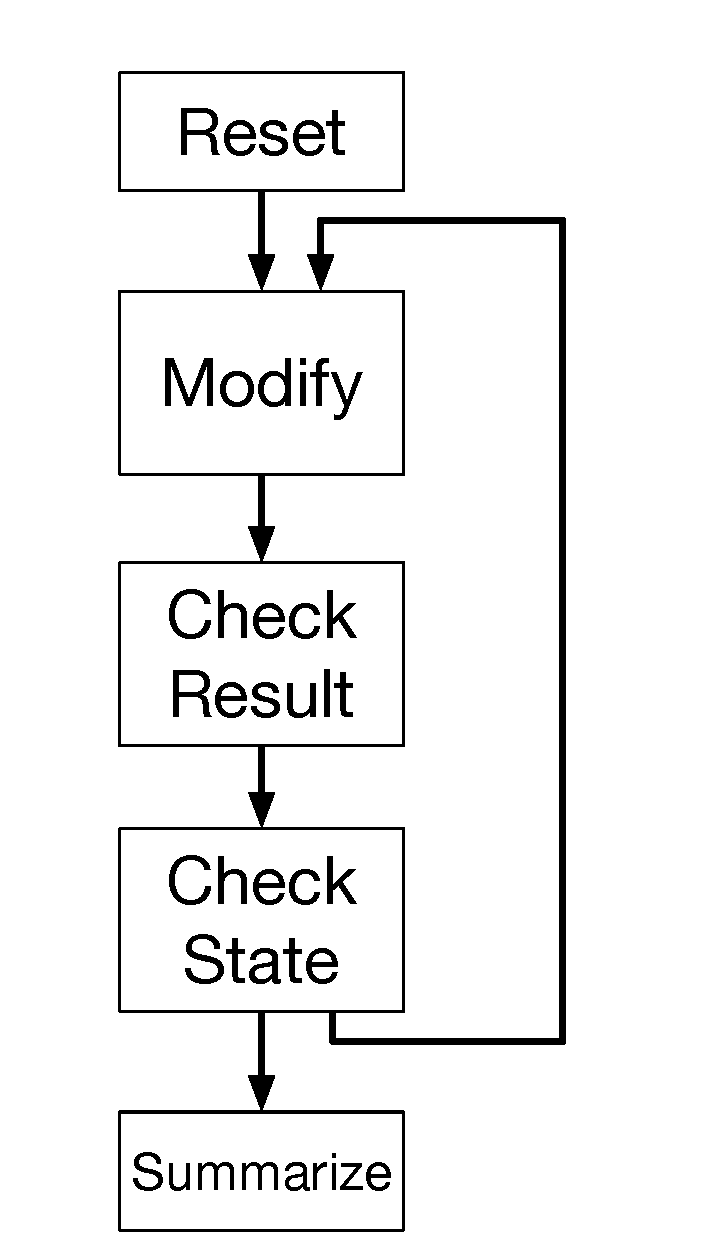
\includegraphics[height=.9\textheight]{images/Comparator-7.pdf}
}

\only<8>{
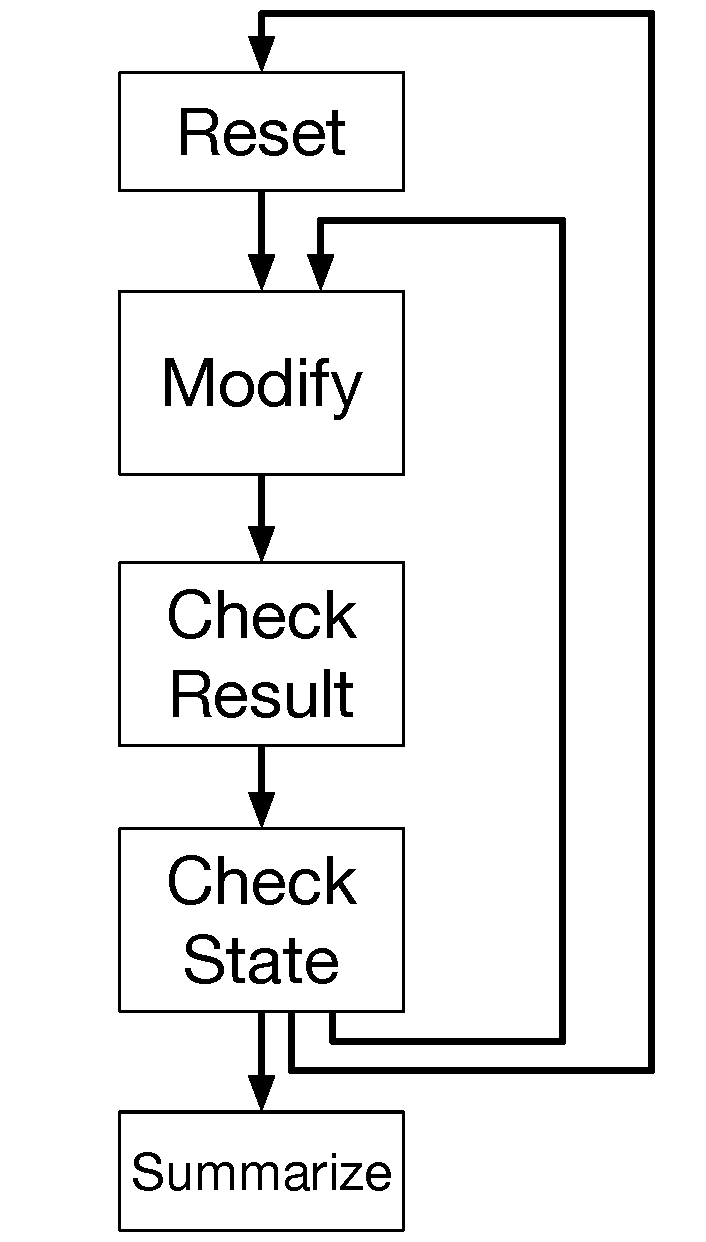
\includegraphics[height=.9\textheight]{images/Comparator-8.pdf}
}
\end{center}

\end{frame}


%%%%%%%%%%%%%%%%%%%%%%%%%%%%%%%%%%%%%%%%%%%%%%%%%%
\begin{frame}[fragile]{}

\begin{center}
{\Huge
Comparator Implementation
}
\end{center}

\end{frame}

\begin{frame}[fragile]{Pet Generator}

\begin{lstlisting}[language=JavaScript]
const chooseFrom = arr => arr[Math.floor(arr.length * Math.random())];

const possibleNames = ['A', 'B', 'C'];
const possibleSpecies = ['Cat', 'Dog', 'Canary', 'Rabbit', 'Fish'];

const name = () => chooseFrom(possibleNames);
const price = () => Math.floor(150 * Math.random());
const species = () => chooseFrom(possibleSpecies);

const randomPet = () => 
          ({petName: name(), petPrice: price(), petType: species()});
\end{lstlisting}

\end{frame}

\begin{frame}[fragile]{Request Generator}

\begin{lstlisting}[language=JavaScript]
const resets = [
    // delete all pets
    () => ({url: '/reset', method: 'DELETE'}),
];

const modifyingRequestGenerator = [
    // addPet
    () => ({url: '/pets', method: 'POST', json: true, body: randomPet()}),
    // removePet
    () => ({url: '/pets', method: 'DELETE', json: true, body: randomPet()})
];

const comparisons = [
    // getPets
    () => ({url: '/pets', method: 'GET'}),
];
\end{lstlisting}

\end{frame}

\begin{frame}[fragile]{Query Submission}

\begin{lstlisting}[language=JavaScript]
const backend = {baseURL: 'http://localhost:9090'};
const essence = {baseURL: 'http://localhost:8080'};

const merge = (req, server) => 
        Object.assign({}, req, {url: server.baseURL + req.url});

const requestFunctionFor = (req, server) =>
    callback => request(merge(req, server), 
                        (err, response) => callback(err, response.body));

const runRequest = (req, callback) => {
    console.log('Now checking:', req);
    async.parallel({
        backend: requestFunctionFor(req, backend),
        essence: requestFunctionFor(req, essence)
    }, callback);
};
\end{lstlisting}

\end{frame}

\begin{frame}[fragile]{Request-Compare-Loop}

\begin{lstlisting}[language=JavaScript]
const requestAndCompare = (request, mainCallback) => {

    console.log('Running the modification request:');

    runRequest(request, (err, result) => {
        const backendString = JSON.stringify(result.backend);
        const essenceString = JSON.stringify(result.essence);
        
        if (backendString !== essenceString) {
            mainCallback('Backend and Essence responses differ! Backend: ' + backendString + ' - Essence: ' + essenceString);
            
        } else {
            
            console.log('Comparing all data:');
            compareEverything(mainCallback);
        }
    });
};
\end{lstlisting}

\end{frame}


\begin{frame}[fragile]{Comparisons}

\begin{lstlisting}[language=JavaScript]
function compareEverything(mainCallback) {
    async.map(comparisons, (itemFunc, callback) => 
        runRequest(itemFunc(), (err, res) => {
            if (res.backend === res.essence) {
                callback(null, null); // no differences
            } else {
                const formatDiff = formatter.formatDiff({
                    backend: JSON.parse(res.backend),
                    essence: JSON.parse(res.essence)
                });
                callback(null, formatDiff);
            }
        }),
        (err, results) => {
            const nonmatching = results.filter(x => x);
            mainCallback(nonmatching.length
                    ? 'Backend and Essence differ in their data' : null);
        });
}
\end{lstlisting}

\end{frame}



\begin{frame}[fragile]{The Main Loop}

\begin{lstlisting}[language=JavaScript]
const requests = [resets[0]()]; // initial reset

let count = 0;

while (count < 50) {
    count++;
    requests.push(chooseFrom(modifyingRequestGenerator)());
}

async.mapSeries(requests, requestAndCompare, (err, results) => {
    results.map(result => console.log(result));
    if (err) {
        console.log(err);
    }
});
\end{lstlisting}

\end{frame}


%%%%%%%%%%%%%%%%%%%%%%%%%%%%%%%%%%%%%%%%%%%%%%%%%%
\begin{frame}[fragile]{Error Discovery in CDCT}

\begin{itemize}[<+->]
\item Backend may discover mismatches
\item Maybe contract has an error
\item Might happen late during development
\end{itemize}

\end{frame}

\begin{frame}[fragile]{Error Discovery in ``Beyond CDCT''}

\begin{itemize}[<+->]
\item We can run comparator against model
\item This may indicate oversights in model
\item Right at the start before development even begins
\end{itemize}

\end{frame}

%%%%%%%%%%%%%%%%%%%%%%%%%%%%%%%%%%%%%%%%%%%%%%%%%%
\begin{frame}[fragile]{}

\begin{center}
{\Huge
What can we discover?
}
\end{center}

\end{frame}


\begin{frame}[fragile]{}

\begin{center}
\only<1>{
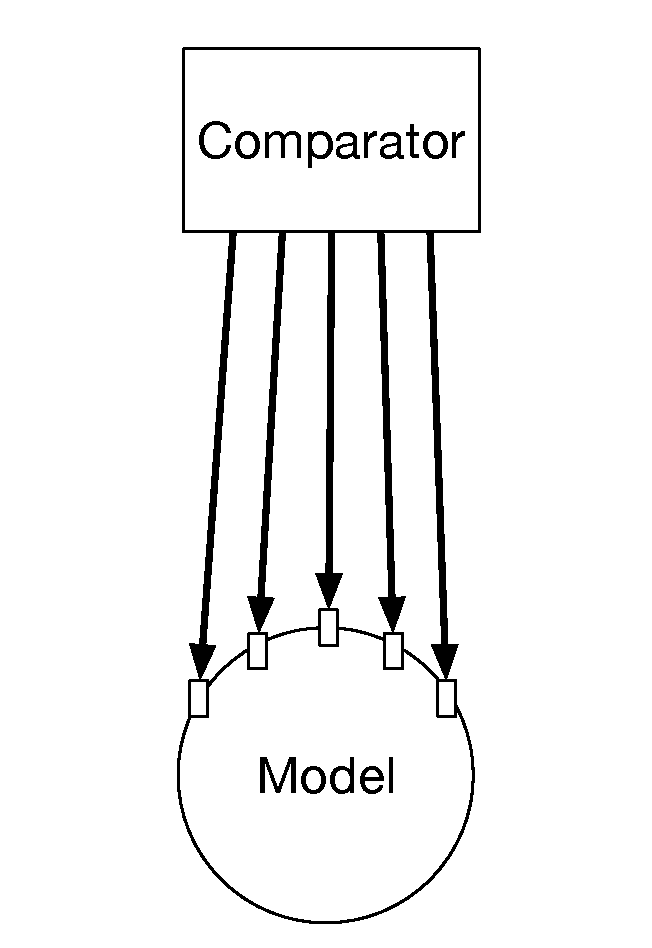
\includegraphics[height=.9\textheight]{images/Issues-0.pdf}
}

\only<2>{
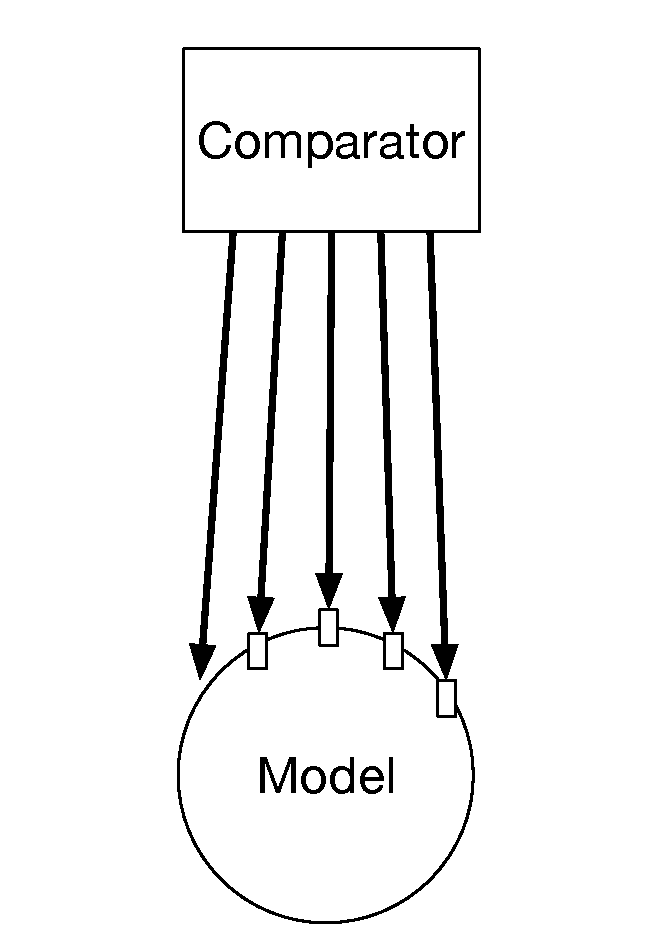
\includegraphics[height=.9\textheight]{images/Issues-1.pdf}
}

\only<3>{
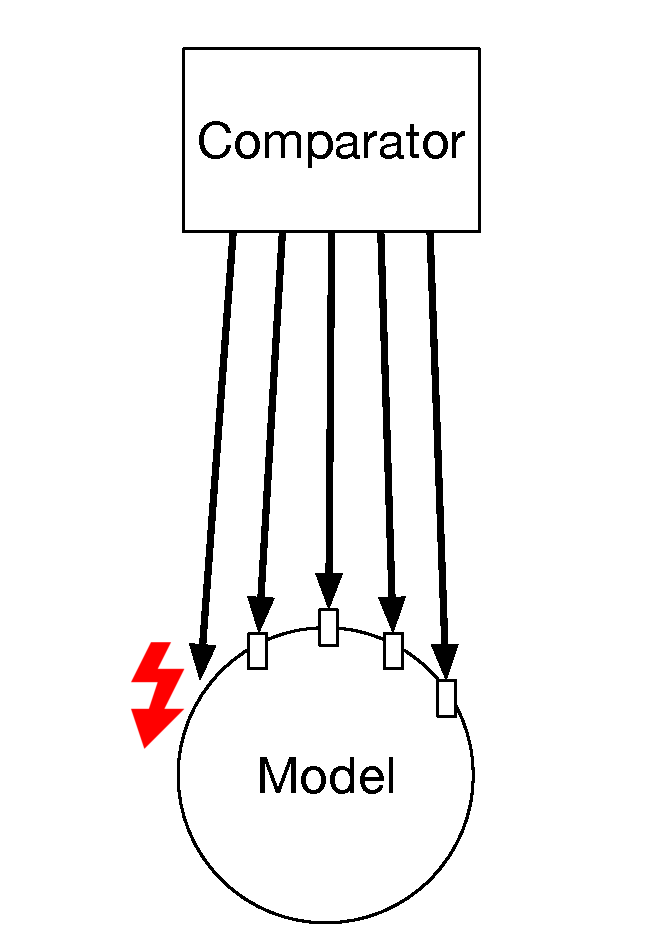
\includegraphics[height=.9\textheight]{images/Issues-1-2.pdf}
}

\only<4>{
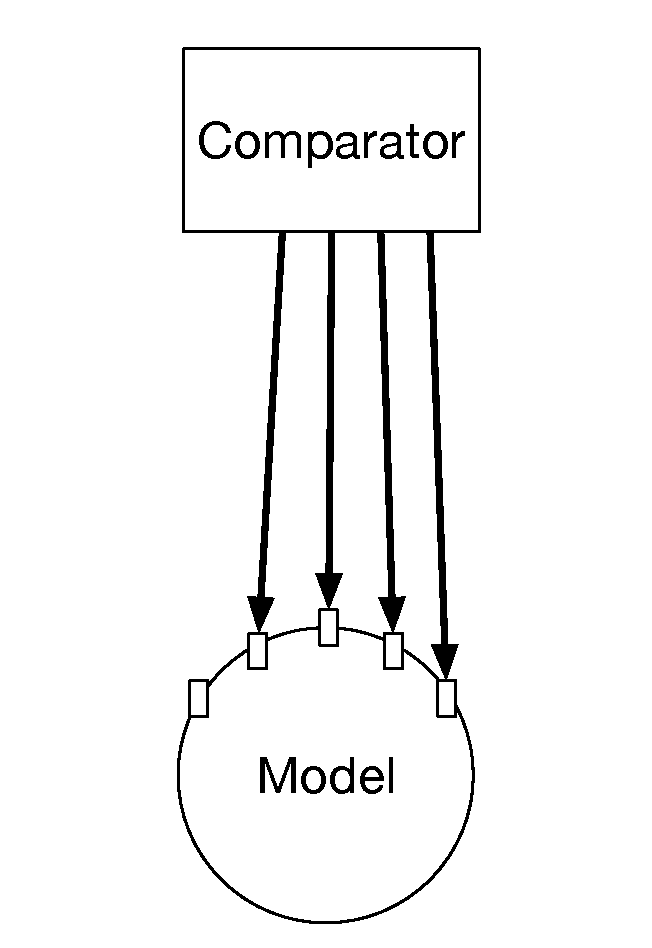
\includegraphics[height=.9\textheight]{images/Issues-2.pdf}
}

\only<5>{
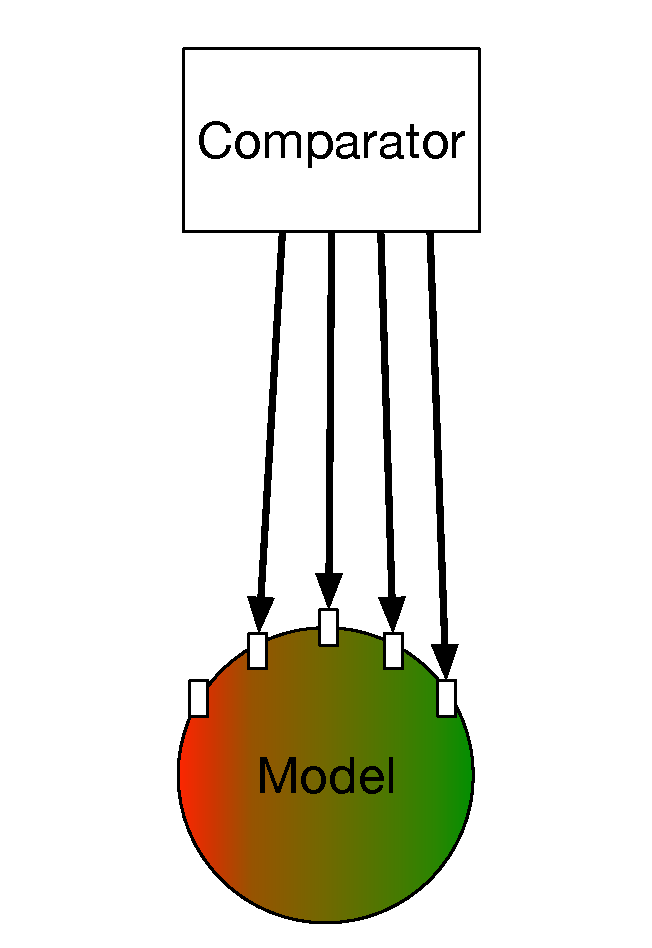
\includegraphics[height=.9\textheight]{images/Issues-2-2.pdf}
}
\end{center}

\end{frame}


%%%%%%%%%%%%%%%%%%%%%%%%%%%%%%%%%%%%%%%%%%%%%%%%%%
\begin{frame}[fragile]{Management Summary}

???

\end{frame}


%%%%%%%%%%%%%%%%%%%%%%%%%%%%%%%%%%%%%%%%%%%%%%%%%%
\begin{frame}{Thank you very much!}

  ~\\[1em]
  \begin{block}{Nicole Rauch}
    \begin{description}[Twitterxx]
    \item[E-Mail]  \href{mailto:info@nicole-rauch.de}{\texttt{info@nicole-rauch.de}}
    \item[Twitter] \href{http://twitter.com/NicoleRauch}{\texttt{@NicoleRauch}}
    \item[Web] \href{http://www.nicole-rauch.de}{\texttt{http://www.nicole-rauch.de}}
    \end{description}
  \end{block}
\end{frame}


%%%%%%%%%%%%%%%%%%%%%%%%%%%%%%%%%%%%%%%%%%%%%%%%%%
\begin{frame}{Credits}

Essence: Mark Morgan - Perfume
{\footnotesize \url{https://www.flickr.com/photos/markmorgantrinidad/5959461561}}


\end{frame}

\end{document}
